% main.tex -- NTU presentation: ultrathin W-doped In2O3 transistors, first-principles inputs and device simulation.
% Build: bash tools/build.sh  ->  build/main.pdf.  Sections are in sections/NN_*.tex (one file per part).
% Authoring rules for every section: AUTHORING_GUIDE.md.
\documentclass[aspectratio=169,10pt]{beamer}
\usepackage{ntutalk}
\addbibresource{../../report_latex_full/references.bib}
\addbibresource{../../report_latex_full/bib/extra_DFT.bib}
\addbibresource{../bib/monograph.bib}
\graphicspath{{figures/}{../figures/}{../../report_latex_full/figures/}{../../qe_workflow/analysis_2026-10-13_full/figures/}%
  {../../qe_workflow/analysis_2026-10-13_full/bands_masses/figures/}{../../analysis_2026-10-06_extraction/figures/final/}%
  {../../analysis_2026-10-06_extraction/figures/paper/}{../../analysis_2026-10-06_extraction/figures/}}

\title{Thickness-Dependent Electronic Structure and Transport\\in Ultrathin W-Doped \InO{} Thin-Film Transistors}
\subtitle{First-principles inputs, device simulation and registered tests}
\author{Mahmoud Elrasheedy}
\date{National Taiwan University \textperiodcentered{} October 2026}

\begin{document}
% 00_title.tex -- title slide and outline (written by hand; not generated).
{\setbeamertemplate{footline}{}
\begin{frame}[plain,noframenumbering]
  \begin{tikzpicture}[remember picture,overlay]
    \node[anchor=north west,inner sep=0] at ($(current page.north west)+(10mm,-8mm)$) {\ntuheader{11mm}};
    \draw[ntumaroon,line width=0.6pt] ($(current page.north west)+(10mm,-23mm)$) -- ($(current page.north east)+(-10mm,-23mm)$);
    \node[anchor=north west,inner sep=0,text width=140mm,align=left] at ($(current page.north west)+(10mm,-31mm)$) {%
      {\Large\bfseries Thickness-Dependent Electronic Structure and Transport\\[1mm]
       in Ultrathin W-Doped \InO{} Thin-Film Transistors\par}
      \vspace{3mm}
      {\normalsize\color{inkgrey} First-principles inputs, device simulation and registered tests\par}
      \vspace{9mm}
      {\small\textbf{Mahmoud Elrasheedy}\par}
      \vspace{1.2mm}
      {\footnotesize Advisor: Prof.\ Chao-Hsin Wu \quad\textperiodcentered\quad Mentor: Mukul Kumar\par}
      \vspace{0.6mm}
      {\footnotesize National Taiwan University\par}
    };
    \draw[rulegrey,line width=0.4pt] ($(current page.south west)+(10mm,17mm)$) -- ($(current page.south east)+(-10mm,17mm)$);
    \node[anchor=north west,inner sep=0,text width=140mm,align=left] at ($(current page.south west)+(10mm,15mm)$) {%
      {\scriptsize\color{inkgrey} Device data: Prof.\ Min-Hung Lee's group, National Taiwan University
        (M.~Januar, Z.-F.~Luo; with K.-C.~Liu, Chang Gung University)\par}
      \vspace{0.8mm}
      {\scriptsize\color{inkgrey} October 2026 \quad\textperiodcentered\quad Unpublished results\par}
    };
  \end{tikzpicture}
\end{frame}}

\begin{frame}{Outline}
  \begin{columns}[T]
    \begin{column}{0.48\linewidth}
      \begin{enumerate}\small
        \item Motivation: ultrathin oxide channels
        \item Devices and measured data
        \item Research questions and registered tests
        \item Device simulation: what calibration can and cannot show
        \item First-principles methods
        \item Quantum confinement of crystalline \InO{} films
        \item Electron and hole masses
      \end{enumerate}
    \end{column}
    \begin{column}{0.48\linewidth}
      \begin{enumerate}\small\setcounter{enumi}{7}
        \item Tungsten as a donor
        \item Oxygen vacancies near W
        \item From first principles to the device
        \item Amorphous films: the registered protocol
        \item Alternative explanations and uncertainty
        \item Computational cost
        \item Conclusions and next steps
      \end{enumerate}
    \end{column}
  \end{columns}
  \vfill
  {\scriptsize\color{inkgrey} Evidence labels used throughout: \textsc{measured}, \textsc{derived}, \textsc{fitted},
  \textsc{computed}, \textsc{observed}, \textsc{assumed}, \textsc{inferred}, \textsc{hypothesis}, \textsc{theory},
  \textsc{unresolved}, \textsc{falsified}. Results that are sealed under the
  registered release protocol are shown as placeholders only.\par}
\end{frame}

% 01_motivation.tex -- Part 1, motivation. Sources: research_monograph/chapters/M01_introduction.tex (scaling, BEOL, In2O3
% at the thickness limit, research problem, approach), M03_literature_materials.tex (W and amorphous-oxide literature),
% M10_w_and_vacancies.tex (C023: the paper's crystalline DFT did not test vacancy passivation), M14_audit.tex (published
% crystalline PBE of In2O3 and W:In2O3), M02_questions.tex and M08_c10_campaign.tex (register, shared model, stages
% S0-S7, S0/S1 seen before the freeze, donor density fixed at the model V1 value), M04_dft_theory.tex (HSE06 checks),
% M12_multiscale.tex (transfer table: W treated as fully ionised, no donor density transferred), M15_conclusions.tex
% (6.3 nm out-of-sample misses), 03_device_data_rev.tex and M07_provenance.tex (published mobilities, pp. 3, 7),
% 11_validation_rev.tex (per-film misses), evidence/FACT_REGISTRY.tsv (FACT-101..104), CLAIM_SOURCE_MAP.tsv (C002, C010,
% C012-C014, C016, C023, C029, M007: 2.0-13.2 nm step -0.579 V, 2.0 -> 6.3 nm -0.018 V).
% Deck rules (AUTHORING_GUIDE section 8): step terminology G4 is defined on the problem slide; at most three footnote
% lines per slide (G6), so works cited for consecutive statements share one footnote; no \sref inside \src (G3).
\providecommand{\oneTop}{\vspace{-3mm}}

\partslide{Part 1}{Motivation: ultrathin oxide channels}

% ---------------------------------------------------------------------------------------------------------------------
\begin{frame}{Upper transistor tiers must be processed below about 400\,\textdegree C}
  \oneTop
  \begin{columns}[T,onlytextwidth]
    \begin{column}{0.60\textwidth}
      \begin{itemize}
        \item Geometric scaling has slowed since the end of Dennard scaling, and thinned channels lose performance:
          Si below about 3\,nm, InGaAs below about 10\,nm\footnote[frame]{\refcite{Theis2017}; \refcite[p.~164]{Si2022}}.
        \item Monolithic 3-D integration stacks back-end-of-line (BEOL) transistor tiers above the Cu interconnect,
          which limits their processing to below about 400\,\textdegree C\sref[p.~1]{Januar2026}.
        \item This excludes crystalline Si; oxide semiconductors are the leading candidates. Their low off-current
          enables capacitor-less DRAM with retention beyond 400\,s\srefs{Datta2019,Belmonte2020}.
      \end{itemize}
    \end{column}
    \begin{column}{0.36\textwidth}
      \centering
      \vspace{1mm}
      \begin{tikzpicture}[x=1mm,y=1mm,line width=0.5pt,font=\scriptsize]
        \draw (0,0) rectangle (36,6);   \node at (18,3) {Si substrate};
        \draw (0,6) rectangle (36,13);  \node at (18,9.5) {Si CMOS logic};
        \draw (0,13) rectangle (36,29);
        \foreach \y in {16.5,21,25.5} {\draw[inkgrey] (3,\y) -- (10,\y); \draw[inkgrey] (26,\y) -- (33,\y);}
        \foreach \x in {6,30} {\draw[inkgrey] (\x,13) -- (\x,29);}
        \node[align=center] at (18,21) {Cu\\interconnect};
        \draw[ntumaroon,line width=0.8pt] (0,29) rectangle (36,37);
        \node[align=center] at (18,33) {oxide-channel\\transistor tier};
        \draw[inkgrey] (0,37) rectangle (36,42); \node[inkgrey] at (18,39.5) {upper interconnect};
        \draw (37,42) -- (38.5,42) -- (38.5,29) -- (37,29);
        \node[anchor=west,align=left] at (39,35.5) {below\\400\,\textdegree C};
      \end{tikzpicture}
      \src{Schematic of a monolithic 3-D stack, not to scale.}
    \end{column}
  \end{columns}
  \takeaway{Oxide semiconductors are the leading channel candidates for the upper tiers.}
\end{frame}

% ---------------------------------------------------------------------------------------------------------------------
\begin{frame}{Indium oxide switches off only as a film a few nanometres thick}
  \oneTop
  \begin{columns}[T,onlytextwidth]
    \begin{column}{0.46\textwidth}
      {\small\textbf{Why oxide and \InO{} channels}\par}
      \begin{itemize}
        \item Amorphous oxides were developed for display transistors; their s-like conduction band survives
          disorder\srefs{Nomura2004,Medvedeva2017}.
        \item \InO{} switches off only when very thin: atomic-layer-deposited 0.7\,nm channels work in enhancement mode,
          with a threshold tuned by thickness and attributed to confinement. Nanometre-thick \InO{} carries drain
          currents above 10\,A/mm\footnote[frame]{\refcite[p.~500]{Si2021}; \refcite[p.~21536]{Lin2022}}.
      \end{itemize}
    \end{column}
    \begin{column}{0.50\textwidth}
      {\small\textbf{What thinning costs}\par}
      \begin{itemize}
        \item Confinement opens the gap and moves the band edges (Part~6) \lab{computed}.
        \item Every atom is near a surface; conventional amorphous oxides become disorder-limited below about
          10\,nm\sref[p.~1]{Januar2026}.
        \item Device spread grows as donors become few: about 500 per \textmu m$^{2}$ in a 2.0\,nm channel at the
          calibrated effective density \num{2.5e17}\cmcu{} (not identifiable from $\Id$--$\Vg$) \lab{fitted}.
      \end{itemize}
    \end{column}
  \end{columns}
  \takeaway{Thin \InO{} switches off; confinement, surfaces and few donors then shape the device.}
\end{frame}

% ---------------------------------------------------------------------------------------------------------------------
\begin{frame}{W keeps \InO{} mobile; its role in nanometre-thin films is open}
  \oneTop
  {\scriptsize\renewcommand{\arraystretch}{1.0}%
  % plain tabular (not tabularx): tabularx typesets its body several times and would repeat the footnote citations.
  % Footnote [1] holds the three W:In2O3 film and transistor studies (rows 1-3), [2] Swallow, [3] the device paper.
  \begin{tabular}{@{}>{\raggedright\arraybackslash}p{2.95cm}>{\raggedright\arraybackslash}p{2.45cm}%
      >{\raggedright\arraybackslash}p{\dimexpr\textwidth-5.4cm-4\tabcolsep\relax}@{}}
    \toprule
    Work & System & Finding used here \\\midrule
    Newhouse et al.\ 2005\srefs{Newhouse2005,Kizu2014,Kim2024} & W:\InO{} (IWO) films & high Hall mobility at
      substantial carrier density \\
    Kizu et al.\ 2014\footnotemark[1] & a-In--W--O TFTs & a few \% W: high mobility and stability at low process
      temperature \\
    Kim et al.\ 2024\footnotemark[1] & IWO TFTs & stability depends on channel thickness \\
    Swallow et al.\ 2020\sref{Swallow2020} & Mo:\InO{} & Mo 4d states high in the conduction band (resonant doping) \\
    Januar et al.\ 2026\sref{Januar2026} & IWO, about 2\,\% W & 2.0--13.2\,nm devices; analytic model fitted per
      device; crystalline PBE cells of \InO{} and W:\InO{} \\
    \bottomrule
  \end{tabular}\par}
  \vspace{0.5mm}
  \begin{itemize}
    \item The device paper\footnotemark[3] (pp.~3, 4, 7) reports that W passivates oxygen vacancies, and relates the
      fall of the peak mobility from about 27.4 to 5.1\cmVs{} (13.2 to 2.0\,nm) to a roughly fourfold rise of the trap
      density.
    \item Apart from that paper's crystalline cells, the project's literature search found no peer-reviewed DFT study
      of W in \InO{}; those cells did not test the vacancy-passivation statement.
  \end{itemize}
  \takeaway{Whether W passivates vacancies in \InO{} is open; Parts~8 and 9 add crystalline tests.}
\end{frame}

% ---------------------------------------------------------------------------------------------------------------------
\begin{frame}{The 2.0--13.2\,nm threshold step ($-0.58$\,V) is fitted, not explained}
  \oneTop
  \begin{columns}[T,onlytextwidth]
    \begin{column}{0.32\textwidth}
      \vspace{1mm}
      {\small
      \begin{tabular}{@{}r r r@{}}
        \toprule
        $t$ (nm) & $\Vthcc$ (V) & $\Delta\Vthcc$ (V) \\\midrule
        2.0  & 0.662 &  \\
        6.3  & 0.644 & \num{-0.018} \\
        13.2 & 0.083 & {\color{ntumaroon}\num{-0.561}} \\\midrule
        \multicolumn{2}{@{}l}{2.0\,$\to$\,13.2\,nm} & \num{-0.579} \\
        \bottomrule
      \end{tabular}\par}
      \vspace{0.5mm}\lab{derived}
      \src{Constant-current threshold at $\Id = 10^{-9}$\,A/\textmu m, $\Vd = 0.7$\,V (registered extraction);
        $\Delta$: change from the next thinner film; last row: the 2.0--13.2\,nm step. One device per film. A 31.8\,nm
        curve, supplied with the data but not part of the published 2.0--13.2\,nm series, never falls below
        $10^{-9}$\,A/\textmu m. Data: Prof.\ M.-H.\ Lee's group, NTU (device paper, footnote~1).}
    \end{column}
    \begin{column}{0.66\textwidth}
      \begin{itemize}
        \item \textbf{The 2.0--13.2\,nm step} is $\Delta\Vthcc = -0.58$\,V. Of it, $-0.56$\,V lies between 6.3 and
          13.2\,nm (\textbf{the 6.3--13.2\,nm drop}); from 2.0 to 6.3\,nm the threshold changes by only $-0.018$\,V
          \lab{derived}.
        \item The device paper\sref{Januar2026} fits eight parameters per device. This project's per-film models match
          each threshold and on-current by construction \lab{fitted}, yet miss the 6.3\,nm on-state shape and the
          13.2\,nm swing \lab{computed}.
        \item All three out-of-sample predictions of the 6.3\,nm threshold failed, missing by $-0.29$, $-0.37$ and
          $-0.23$\,V \lab{falsified}.
        \item A shared model needs material inputs instead: chiefly $\dEc(t)$ (affinity, hence $\Vth$), $m^{*}(t)$
          (density of states, band mobility) and whether W is ionised (its share of the carriers).
      \end{itemize}
    \end{column}
  \end{columns}
  \takeaway{The question: which of these inputs can first principles supply to one shared model?}
\end{frame}

% ---------------------------------------------------------------------------------------------------------------------
\begin{frame}{This work: computed inputs, a shared model, registered tests}
  \oneTop
  {\centering
  \begin{tikzpicture}[x=1mm,y=1mm,font=\scriptsize,line width=0.5pt,
      box/.style={draw,align=center,inner sep=1.2mm,minimum height=8mm},
      arr/.style={-{Stealth[length=2mm]},line width=0.6pt}]
    \node[box,text width=44mm] (meas) at (23.2,20) {\textbf{Measured transfer curves}\\4 films, 2.0--31.8\,nm};
    \node[box,text width=40mm] (extr) at (75,20) {\textbf{Registered extraction}\\$\Vthcc$, swing, mobility, floor};
    \node[box,text width=33mm] (cmp) at (122,20) {\textbf{Comparison}\\against registered criteria};
    \node[box,text width=44mm,align=left] (dft) at (23.2,4) {\textbf{First principles} (PBE; HSE06 checks)\\
      crystalline films 0.46--1.96\,nm\\ W and O vacancies in crystalline cells\\
      amorphous films 0.7--2.0\,nm (sealed)};
    \node[box,text width=40mm] (inp) at (75,4) {\textbf{Device inputs}\\$\dEc(t)$, $\dEg(t)$, $\Delta m^{*}(t)$:
      laws fitted to computed points;\\W taken as fully ionised \lab{inferred}};
    \node[box,text width=33mm] (tcad) at (122,4) {\textbf{Shared-parameter model}\\campaign C10, drift--diffusion;\\
      one set for 2.0, 6.3, 13.2\,nm};
    \draw[arr] (meas) -- (extr);
    \draw[arr] (extr) -- (cmp);
    \draw[arr] (dft) -- (inp);
    \draw[arr,ntumaroon] (inp) -- (tcad);
    \draw[arr] (tcad) -- (cmp);
  \end{tikzpicture}\par}
  \src{Project workflow. Maroon arrow: quantities transferred from first principles to the device model.}
  {\footnotesize\textbf{Legend.} Device campaign C10 runs in stages S0 to S7 (Part~4); results from stage S2 on are
    sealed.\par}
  \begin{itemize}\footnotesize
    \item Five fitted parameters are shared by the 2.0, 6.3 and 13.2\,nm films (a sixth only in the percolation-mobility
      branch); no film-specific charge or mobility.
    \item Tests were registered before their outcomes where possible (Part~3): register revision~2 was frozen on
      10 October 2026, after stages S0 and S1 had been seen. No holdout device exists, so all comparisons are
      retrospective.
  \end{itemize}
  \takeaway{First principles supplies the confinement laws, not the donor density or traps.}
\end{frame}

% 02_device_data.tex -- Part 2: devices and measured data. Sources: research_monograph/chapters/03_device_data_rev.tex,
% chapters/M07_provenance.tex, evidence/derived/device_facts.json, evidence/derived/musat_ratio.json,
% evidence/FACT_REGISTRY.tsv (FACT-100..104, FACT-111..113), evidence/CLAIM_SOURCE_MAP.tsv (M008),
% research_record/03_CLAIMS_LEDGER.yaml (C001-C005, C008, C011, C012, C024-C033), research_record/05_DECISION_LOG.md
% (D-05), analysis_2026-10-06_extraction/PROTOCOL.md (incl. amendment A1 and its disclosure) and results_a1.json.
% Figures 02_*.pdf are drawn by tools/fig_02_device.py from data/experimental_clean.csv.
% Ledger IDs: shown (small, grey) after bullet-level results only; IDs of table rows are given in the \src lines.
% Slide 1 table: C-V (paper SI) = FACT-100 / tab:inp-stack; T = 300 K and the A/um unit: tab:inp-stack, C033.
\providecommand{\twoC}[1]{{\tiny\color{inkgrey}\,#1}}
\providecommand{\twoAum}{\si{A/\micro\metre}}
\providecommand{\twoData}{Data: Prof.\ M.-H.\ Lee's group, NTU; one device per thickness, one sweep (no~reverse~sweep)}
\providecommand{\twoTop}{\vspace{-3mm}}
\providecommand{\twoDataShort}{Data: Prof.\ M.-H.\ Lee's group, NTU}
\providecommand{\twoMusat}{\texorpdfstring{$\mu_\mathrm{sat}$}{mu-sat}}

\partslide{Part 2}{Devices and measured data}

% ---------------------------------------------------------------------------------------------------------------------
\begin{frame}[t]{One nominal stack, four IWO thicknesses, one device each}
  \twoTop
  \begin{columns}[T,onlytextwidth]
    \begin{column}{0.38\textwidth}
      \centering
      \vspace{2mm}
      \begin{tikzpicture}[x=1mm,y=1mm,font=\scriptsize]
        % substrate and gate stack (bottom to top), not to scale
        \filldraw[draw=black,fill=black!22,line width=0.4pt] (0,0) rectangle (52,4);
        \node at (26,2) {n$^+$ Si support};
        \filldraw[draw=black,fill=black!45,line width=0.4pt] (0,4) rectangle (52,10);
        \node[white] at (26,7) {TiN gate, 50\,nm};
        \filldraw[draw=black,fill=black!10,line width=0.4pt] (0,10) rectangle (52,16);
        \node at (26,13) {\HfO{}, 15\,nm, $\varepsilon_r = 19.57$};
        \filldraw[draw=black,fill=white,line width=0.4pt] (0,16) rectangle (52,20);
        \node at (26,18) {\AlO{}, 2\,nm, $\varepsilon_r = 9.0$};
        \filldraw[draw=black,fill=ntumaroon!18,line width=0.4pt] (0,20) rectangle (52,25);
        \node at (26,22.5) {IWO, $t$ = 2.0 / 6.3 / 13.2 / 31.8\,nm};
        % Pd top contacts
        \filldraw[draw=black,fill=black!65,line width=0.4pt] (0,25) rectangle (10,30);
        \filldraw[draw=black,fill=black!65,line width=0.4pt] (42,25) rectangle (52,30);
        \node[white] at (5,27.5) {Pd};
        \node[white] at (47,27.5) {Pd};
        \node[above] at (5,30) {source};
        \node[above] at (47,30) {drain};
        \node at (26,27.3) {air, no passivation};
        % channel length
        \draw[{Latex[length=1.4mm]}-{Latex[length=1.4mm]},line width=0.4pt] (10,32.5) -- (42,32.5);
        \node[fill=white,inner sep=1pt] at (26,32.5) {$L = 20\,\si{\micro\metre}$};
      \end{tikzpicture}\par
      \raggedright
      \src{Not to scale; $W = 290\,\si{\micro\metre}$ into the page. Thicknesses are nominal; their measurement
        method is not reported. ``About 2\,\% W'' is not defined as an atomic or a weight fraction.}
    \end{column}
    \begin{column}{0.59\textwidth}
      {\scriptsize
      \setlength{\tabcolsep}{3pt}
      \renewcommand{\arraystretch}{1.04}
      \begin{tabular}{@{}llll@{}}
        \toprule
        Item & Value & Label & Source \\
        \midrule
        Gate & TiN, 50\,nm, on n$^+$ Si & \lab{measured} & schematic \\
        Gate dielectric & \HfO{}, 15\,nm & \lab{measured} & schematic \\
        \quad permittivity & $\varepsilon_r = 19.57$ & \lab{measured} & C--V (paper SI) \\
        Interlayer & \AlO{}, 2\,nm & \lab{measured} & schematic \\
        \quad permittivity & $\varepsilon_r = 9.0$ & \lab{assumed} & -- \\
        Stack order & \AlO{} at the channel & \lab{assumed} & schematic only \\
        Channel & sputtered IWO, $\approx$2\,\% W & \lab{measured} & paper, schematic \\
        Contacts & Pd, 70\,nm, on top & \lab{measured} & schematic \\
        Above channel & air, no capping layer & \lab{measured} & paper, schematic \\
        $W/L$ & 290\,\si{\micro\metre} / 20\,\si{\micro\metre} & \lab{measured} & schematic \\
        Drain bias & $\Vd = 0.7$\,V (transfer) & \lab{measured} & schematic \\
        Temperature & 300\,K & \lab{assumed} & not recorded \\
        Current unit & \twoAum & \lab{inferred} & schematic axis \\
        \bottomrule
      \end{tabular}\par}
      \src{Schematic and workbook supplied with the data. Process: device paper\sref[pp.~2--3]{Januar2026};
        $\varepsilon_r$(\HfO{}) from its SI, Fig.~S1. The stack order is not stated by the fabrication group; the
        paper's interface calculations use IWO/\HfO{}.}
    \end{column}
  \end{columns}
  \takeaway{Assumed: $\varepsilon_r$(\AlO{}), stack order, 300\,K. Thicknesses nominal; unit \twoAum{} unconfirmed.}
\end{frame}

% ---------------------------------------------------------------------------------------------------------------------
\begin{frame}[t]{Transfer curves: two alike, one shifted, one always on}
  \twoTop
  \begin{columns}[T,onlytextwidth]
    \begin{column}{0.58\textwidth}
      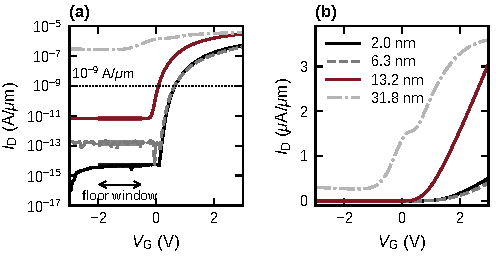
\includegraphics[width=\linewidth]{02_transfer}
      \src{(a) Log scale, line styles as in (b); thick segments: off-state floor (median, $-2 \le \Vg \le -0.5$\,V);
        dotted: $10^{-9}$\,\twoAum. (b) Linear scale. \twoData.}
    \end{column}
    \begin{column}{0.39\textwidth}
      \begin{itemize}\footnotesize
        \item $\Vg$: $-3$ to $+3$\,V, 50\,mV steps, $\Vd = 0.7$\,V; drain current only \lab{measured}\twoC{C001}
        \item 2.0 and 6.3\,nm nearly coincide; 13.2\,nm is shifted to lower $\Vg$, with about six times the
          2.0\,nm on-current \lab{observed}\twoC{C026}
        \item Floors are flat in $\Vg$ and rise steeply with thickness; their origin is open without a gate
          current \lab{observed}
        \item 31.8\,nm never switches off: $\Id(-3\,\mathrm{V}) = 3.0\times10^{-7}$\,\twoAum, on/off about 12
          \lab{derived}\twoC{C029}; outside the published 2--13\,nm series\sref[p.~2]{Januar2026}
      \end{itemize}
    \end{column}
  \end{columns}
  \takeaway{Every trend rests on one sweep of one device per film, with no gate current.}
\end{frame}

% ---------------------------------------------------------------------------------------------------------------------
\begin{frame}[t]{Registered extraction protocol; one disclosed amendment}
  \twoTop
  {\footnotesize
  \renewcommand{\arraystretch}{1.12}
  \begin{tabularx}{\linewidth}{@{}l>{\raggedright\arraybackslash}X@{}}
    \toprule
    Threshold $\Vthcc$ & $\Vg$ at $\Id = 10^{-9}$\,\twoAum{} (290\,nA in total), log-linear interpolation \\
    Off-state floor & median of $\Id$ over $-2 \le \Vg \le -0.5$\,V \\
    Swing (SS) & one decade of current. Registered primary window S1: $[5\times10^{-11}, 5\times10^{-10}]$\,\twoAum;
      secondary window A1, shown here: $[2.15\times10^{-5}, 2.15\times10^{-4}]\,I_\mathrm{on}$,
      $I_\mathrm{on} = \Id(+3\,\mathrm{V})$ \\
    Mobility & $\mu_\mathrm{FE} = L\,g_m/(W C_\mathrm{ox} \Vd)$, $g_m = \partial\Id/\partial\Vg$ (central differences),
      same code for data and simulation; a carrier mobility only if $\Vg - \Vth \ge \Vd$ and $\mu$ is constant \\
    Gate capacitance & $C_\mathrm{ox} = 8.955\times10^{-7}$\,F\,cm$^{-2}$ (EOT 3.86\,nm): 15\,nm \HfO{}
      ($\varepsilon_r$ 19.57) in series with 2\,nm \AlO{} ($\varepsilon_r$ 9.0, assumed) \lab{derived} \\
    \bottomrule
  \end{tabularx}\par}
  \vspace{2mm}
  % timeline: nodes anchored at the baseline of their first line; each dot sits on that first line
  \begin{tikzpicture}[x=1mm,y=1mm,font=\scriptsize,
      tl/.style={anchor=base west,text width=134mm,align=left,inner sep=0pt}]
    \draw[line width=0.5pt] (1,0.75) -- (1,-12.45);
    \fill[ntumaroon] (1,0.75) circle (0.9);
    \fill (1,-4.45) circle (0.7);
    \fill (1,-12.45) circle (0.7);
    \node[tl] at (3.6,0) {6 Oct 2026, decision D-05: protocol committed
      (\texttt{7a61687}), before any data-versus-simulation number of this analysis.};
    \node[tl] at (3.6,-5.2) {After the first results, including the S1
      data--simulation comparison: amendment A1 (\texttt{7ce7116}), as the films' current scales differ.
      Written after its measured values (disclosed), before any simulated value under it.};
    \node[tl] at (3.6,-13.2) {Later (monograph): independent re-implementation
      reproduces thresholds, floors, end-point currents within rounding.};
  \end{tikzpicture}
  \takeaway{Definitions preceded the data--simulation comparison, and A1 preceded any simulated value under it.
    The simulations are calibrated to $\Vthcc$ and $I_\mathrm{on}$: agreement there is not a test.}
\end{frame}

% ---------------------------------------------------------------------------------------------------------------------
\begin{frame}[t]{Threshold is flat to 6.3\,nm, then drops by 0.56\,V}
  \twoTop
  {\centering\footnotesize
  \renewcommand{\arraystretch}{1.0}
  \begin{tabular}{@{}lccccl@{}}
    \toprule
    & 2.0\,nm & 6.3\,nm & 13.2\,nm & 31.8\,nm & \\
    \midrule
    $\Vthcc$ at $10^{-9}$\,\twoAum{} (V) & 0.662 & 0.644 & 0.083 & none & \lab{derived} \\
    Off-state floor (\twoAum) & \num{4.61e-15} & \num{1.53e-13} & \num{6.60e-12} & -- & \lab{derived} \\
    $\Id(+3\,\mathrm{V})$ (\twoAum) & \num{5.09e-7} & \num{4.03e-7} & \num{3.07e-6} & \num{3.59e-6} & \lab{derived} \\
    $\Id(-3\,\mathrm{V})$ (\twoAum) & \num{1.9e-16} & \num{1.9e-13} & \num{6.8e-12} & \num{3.0e-7} & \lab{derived} \\
    $\Id(+3\,\mathrm{V})/\Id(-3\,\mathrm{V})$ & \num{2.7e9}\,$^{\dagger}$ & \num{2.2e6} & \num{4.5e5} & 12
      & \lab{derived} \\
    \bottomrule
  \end{tabular}\par}
  \src{$^{\dagger}$ The 2.0\,nm sweep starts below its floor: not a channel on/off ratio.
    \twoDataShort\sref{Januar2026}; ledger C002, C003, C029; recomputed independently (FACT-101--104).}
  \vspace{-1mm}
  \begin{itemize}\footnotesize
    \item Non-uniform: 2.0\,$\to$\,6.3\,nm changes $\Vthcc$ by $-0.018$\,V and $\Id(+3\,\mathrm{V})$ by $\times0.79$;
      6.3\,$\to$\,13.2\,nm by $-0.561$\,V and $\times7.6$ \lab{observed}\twoC{C026}
    \item The 13.2\,nm floor is 1432 times the 2.0\,nm floor and flat in $\Vg$ within 3\,\%: gate leakage unlikely
      \lab{inferred}\twoC{C005}, but no gate current was recorded
    \item The 2.0\,nm floor, 1.3\,pA in total, is at a measurement-setup level \lab{inferred}\twoC{C003}; no
      instrument floor recorded
  \end{itemize}
  \takeaway{Small change to 6.3\,nm, large to 13.2\,nm: one device per film cannot fix a thickness law.}
\end{frame}

% ---------------------------------------------------------------------------------------------------------------------
\begin{frame}[t]{The published 60--70\,mV/dec appears only next to the floor}
  \twoTop
  \begin{columns}[T,onlytextwidth]
    \begin{column}{0.43\textwidth}
      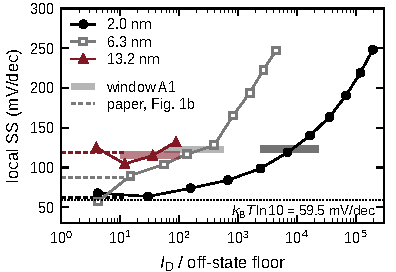
\includegraphics[width=\linewidth]{02_local_ss}
      \src{Local SS $= d\Vg/d\log_{10}\Id$ (central differences), rising branch up to $10^{-9}$\,\twoAum. Bars: window
        A1 and its value. Dashed: paper Fig.~1b value at 1--12 times the floor, where near-floor estimators
        reproduce it; the paper's range is not known. The first 6.3\,nm point lies below $\kT\ln10$, which no
        channel current can do. \twoDataShort.}
    \end{column}
    \begin{column}{0.54\textwidth}
      {\footnotesize
      \setlength{\tabcolsep}{3.5pt}
      \begin{tabular}{@{}lccc@{}}
        \toprule
        SS (mV/dec) & 2.0\,nm & 6.3\,nm & 13.2\,nm \\
        \midrule
        Paper, Fig.~1b & 61.8 & 87.4 & 119.3 \\
        Window A1 & \num{123.6(10)} & \num{122.7(93)} & \num{115.3(24)} \\
        \bottomrule
      \end{tabular}\par}
      \src{Paper values digitised. A1 values derived; A1 is the protocol's secondary window. The registered primary
        window S1 deviates from the paper by up to $+168$\,\% (ledger C008, C032).}
      \begin{itemize}\footnotesize
        \item By its own Fig.~1b, the paper's ``60--70\,mV/dec''\sref[p.~3]{Januar2026} holds at 2.0\,nm only;
          A1 gives twice that \lab{unresolved}\twoC{C025}
        \item Of 31 scored estimator variants, 14 match the paper within 15\,\% if started within 1--12 times the
          floor; the best is an outcome selection, not adopted \lab{derived}\twoC{C032}
        \item A floor $F$ gives $\mathrm{SS}_\mathrm{raw} = \mathrm{SS}_\mathrm{ch}(1 + F/I_\mathrm{ch})$,
          $I_\mathrm{ch}$: channel current. Subtracting $F$ steepens SS by construction; some estimators then fall
          below $\kT\ln10 = 59.5$\,mV/dec at 300\,K \lab{derived}
      \end{itemize}
    \end{column}
  \end{columns}
  \takeaway{Near-thermal switching and a low trap density are not established by these curves.}
\end{frame}

% ---------------------------------------------------------------------------------------------------------------------
\begin{frame}[t]{The \twoMusat{} peak reproduces the published mobilities}
  \twoTop
  \begin{columns}[T,onlytextwidth]
    \begin{column}{0.51\textwidth}
      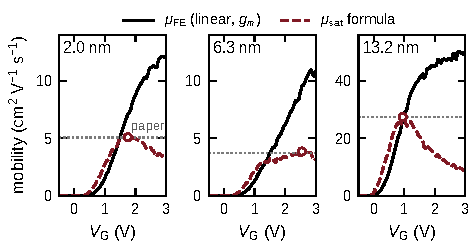
\includegraphics[width=\linewidth]{02_mobility}
      \src{Both formulas on the same curves, $C_\mathrm{ox} = 8.955\times10^{-7}$\,F\,cm$^{-2}$, $W/L = 290/20$,
        $\Vd = 0.7$\,V. Circle: $\mu_\mathrm{sat}$ peak; dotted: paper value. $\mu_\mathrm{sat}$ is one of six
        definitions tested; derivative-estimator spread of its peak 5.04--5.11 / 3.78--3.90 / 25.9--27.5\,\cmVs;
        the $C_\mathrm{ox}$ uncertainty (scales all values) is not included. $\mu_\mathrm{FE}$ peaks at
        $\Vg$ = 3.0 / 2.85 / 2.8\,V. \twoData.}
    \end{column}
    \begin{column}{0.46\textwidth}
      \vspace{-3mm}
      \[ \mu_\mathrm{sat} = \frac{2L}{W C_\mathrm{ox}}\left(\frac{\partial\sqrt{\Id}}{\partial\Vg}\right)^{2} \]\par
      \vspace{-2mm}
      {\footnotesize
      \setlength{\tabcolsep}{4pt}
      \begin{tabular}{@{}lccc@{}}
        \toprule
        cm$^2$\,V$^{-1}$\,s$^{-1}$ & 2.0\,nm & 6.3\,nm & 13.2\,nm \\
        \midrule
        Paper, $\mu_\mathrm{max}$ & 5.1 & 3.73$^{*}$ & 27.4 \\
        $\mu_\mathrm{sat}$ peak & 5.09 & 3.86 & 27.40 \\
        $\mu_\mathrm{FE}$ peak & 12.1 & 10.9 & 50.2 \\
        \bottomrule
      \end{tabular}\par}
      \src{Paper values\sref[pp.~3, 7]{Januar2026}; $^{*}$ digitised from its Fig.~1b. Both lower rows derived.}
      \begin{itemize}\footnotesize
        \item No adjustable factor is needed \lab{derived}\twoC{C030}, so this peak is the leading candidate for
          the paper's definition \lab{inferred}\twoC{C031}
        \item Not an identification: the peaks fix only $C_\mathrm{ox}\,W/L\times$(current unit); $\mu_\mathrm{eff}$
          with power-law threshold and the Y-function also fit, with one common factor (0.68, 0.66)
      \end{itemize}
    \end{column}
  \end{columns}
  \takeaway{A definition difference suffices to reconcile the mobilities; the recipe is unconfirmed.}
\end{frame}

% ---------------------------------------------------------------------------------------------------------------------
\begin{frame}[t]{On linear-regime curves, \twoMusat{} is not a mobility}
  \twoTop
  \begin{columns}[T,onlytextwidth]
    \begin{column}{0.46\textwidth}
      {\footnotesize Linear regime ($V_\mathrm{ov} \ge \Vd$), constant $\mu$, overdrive $V_\mathrm{ov} = \Vg - \Vth$:\par}
      \vspace{-2mm}
      \[ \Id = \mu\,C_\mathrm{ox}\frac{W}{L}\Big(V_\mathrm{ov} - \frac{\Vd}{2}\Big)\Vd \]
      {\footnotesize inserted into the saturation formula:\par}
      \vspace{-2mm}
      \[ \frac{\mu_\mathrm{sat}}{\mu} = \frac{\Vd}{2V_\mathrm{ov} - \Vd} \]
      {\footnotesize Below 1 whenever $V_\mathrm{ov} > \Vd$ and falling as $1/V_\mathrm{ov}$: a low mobility that falls
        with $\Vg$ even when $\mu$ is constant. The saturation formula itself holds only for $V_\mathrm{ov} \le \Vd$.
        \lab{theory}\par}
    \end{column}
    \begin{column}{0.51\textwidth}
      {\footnotesize
      \setlength{\tabcolsep}{4pt}
      \begin{tabular}{@{}lccc@{}}
        \toprule
        At the $\mu_\mathrm{sat}$ peak & 2.0\,nm & 6.3\,nm & 13.2\,nm \\
        \midrule
        $\Vg$ (V) & 1.75 & 2.55 & 0.95 \\
        $V_\mathrm{ov}$ with $\Vthcc$ (V) & 1.09 & 1.91 & 0.87 \\
        $\mu_\mathrm{sat}/\mu_\mathrm{FE}$, constant $\mu$ & 0.47 & 0.22 & 0.68 \\
        $\mu_\mathrm{sat}/\mu_\mathrm{FE}$, observed & 0.72 & 0.41 & 1.02 \\
        \bottomrule
      \end{tabular}\par}
      \src{\twoDataShort\sref{Januar2026}. Ratios derived from the same curves (constant-$\mu$ identity,
        $\Vthcc$); overdrives under all three threshold definitions: ledger C031.}
      \begin{itemize}\footnotesize
        \item With $\Vthcc$ all three peaks lie at $V_\mathrm{ov} > \Vd = 0.7$\,V; with the two other thresholds
          tested, 2.0 and 13.2\,nm can lie inside the range, 6.3\,nm never \lab{derived}
        \item Observed ratios exceed the prediction by 1.5--1.8 \lab{derived}\twoC{M008}, as expected if $\mu$ rises
          with $\Vg$: power-law fits $\mu \propto (\Vg - \Vth)^{\gamma}$ give $\gamma = 0.27\pm0.08$ (13.2\,nm)
          and 1.13 (6.3\,nm) \lab{fitted}\twoC{C011, C012}
      \end{itemize}
    \end{column}
  \end{columns}
  \takeaway{The $\mu_\mathrm{sat}$ peaks are numerical matches, not channel mobilities; nor is $\mu_\mathrm{FE}$
    intrinsic.}
\end{frame}

% 03_questions_registration.tex -- Part 3: research questions and registered tests. Sources: research_monograph/chapters/
% M02_questions.tex (questions, prerequisites, tab:mono-q-map H1-H8 with priors and the H-E status "S1-05 expectation
% failed; rest sealed", governance incl. censoring rule, "exactly one label" rule, A38/A42/A43, A36 erratum, roles),
% M08_c10_campaign.tex (H-A..H-F, H-J, tab:mono-c10-stages S0-S7, S1-05, A13, A22), M11_amorphous_protocol.tex
% (tab:mono-am-tests H-G, H-H, H-I, H-K, H-M, H-N; A27, A37, prop:mono-hn, D-43 release conditions; no electronic
% quantity), M10_w_and_vacancies.tex (H-L registration A17, 80-atom cells, verdict), M14_audit.tex (timestamps, P27);
% appendices/MG_corrections.tex (A36 erratum: disclosed exposure, no value reproduced); evidence/CLAIM_SOURCE_MAP.tsv
% (C006, C007, C010, C014, C019, C027, C028, C038); research_record/05_DECISION_LOG.md (D-11, D-17, D-20/A18 time, D-42,
% D-43); results/RUN_INDEX.csv (stage S0/S1 runs 0061-0074 on 2026-10-10 before 18:33Z).
% The full registered criteria (H-A..H-N, the DONOR class rule) are in sections/16b_backup_register.tex (backup).
% The thickness-step alternatives (M13 tab:mono-alt-tc) are shown once, in Part 12; the swing collapse (H7) in Part 2.
% Blind rules: no sealed outcome, no amorphous electronic quantity, no ATLAS result from stage S2 on.
% Note: every frame body starts with a command (\threeTop), never a brace group (beamer would read a subtitle).
\providecommand{\threeAum}{\si{A/\micro\metre}}
\providecommand{\threeData}{Data: Prof.\ M.-H.\ Lee's group, NTU}
\providecommand{\threeTop}{\vspace{-4mm}}
% evidence label at the start of a table cell (\leavevmode keeps it on the first line of the cell)
\providecommand{\threeLab}[1]{\leavevmode\lab{#1}}
% italic group heading inside a three-column table
\providecommand{\threeGroup}[1]{\multicolumn{3}{@{}l}{\textit{#1}}}

\partslide{Part 3}{Research questions and registered tests}

% ---------------------------------------------------------------------------------------------------------------------
\begin{frame}{One central question, four separate evidence chains}
  \threeTop
  \begingroup\small\textbf{Central question.} \emph{What sets the thickness dependence of ultrathin W-doped \InO{}
    transistors, and can one shared-parameter device model with first-principles inputs account for it?}\par\endgroup
  \vspace{1mm}
  \begingroup\footnotesize
  \renewcommand{\arraystretch}{1.0}
  \begin{tabularx}{\textwidth}{@{}>{\raggedright\arraybackslash}p{2.8cm}>{\raggedright\arraybackslash}X r@{}}
    \toprule
    Evidence chain & Question & Part \\
    \midrule
    1\ \ Electronic structure & How do gap, band edges and electron mass change from bulk to below 1\,nm, and how much
      of the shift is in the conduction band? & 6, 7 \\\addlinespace[0.3mm]
    2\ \ Tungsten & Does W donate into extended host states (crystalline, amorphous), does this change with
      thickness, and does W suppress O vacancies? & 8, 9, 11 \\\addlinespace[0.3mm]
    3\ \ Device physics & Which mechanisms set the threshold, swing, on-current and off-state floor of each film, and
      which of them can a shared model reproduce? & 4, 10 \\\addlinespace[0.3mm]
    4\ \ Provenance & How do our metrics relate to the published ones? What do the data permit? & 2 \\
    \bottomrule
  \end{tabularx}\par\endgroup
  \vspace{1.6mm}
  \begingroup\footnotesize\textbf{Prerequisites that the data cannot settle} (no new measurements are available)\par
  \vspace{0.6mm}
  \begin{tabularx}{\textwidth}{@{}l>{\raggedright\arraybackslash}X@{}}
    Definitions & Same definitions of mobility, swing, $C_\mathrm{ox}$ and $\Vd$ as the paper? Partly answered (Part 2). \\
    Spread & How large is the device-to-device spread? This needs at least ten devices per thickness. \\
    Fabrication & How were thicknesses measured; do the four devices share a run and a sweep history? \\
  \end{tabularx}\par\endgroup
  \takeaway{Each chain is tested separately; the prerequisites need new devices.}
\end{frame}

% ---------------------------------------------------------------------------------------------------------------------
\begin{frame}{No first-pass hypothesis is settled by the evidence so far}
  \threeTop
  \begingroup\scriptsize
  \setlength{\tabcolsep}{3pt}
  \renewcommand{\arraystretch}{1.0}
  \begin{tabularx}{\textwidth}{@{}>{\raggedright\arraybackslash}p{4.95cm}>{\raggedright\arraybackslash}p{1.49cm}%
      >{\raggedright\arraybackslash}p{1.7cm}>{\raggedright\arraybackslash}X r@{}}
    \toprule
    First-pass hypothesis (7 Oct 2026) & Prior & Registered as & Status at the present evidence state & Part \\
    \midrule
    H1\ \ a critical thickness separates two regimes; W shifts it & medium (sharp $t_c$) & -- &
      \threeLab{hypothesis}; one device per film & 12 \\\addlinespace[0.3mm]
    H2\ \ W keeps conduction-edge states delocalised & low--medium & H-G, H-N &
      sealed; H-N cannot return a crossover verdict, by rule & 8, 11 \\\addlinespace[0.3mm]
    H3\ \ the 6.3\,nm anomaly is real physics & low & H-F (shape) &
      \threeLab{hypothesis}; out-of-sample 6.3\,nm threshold predictions failed \lab{falsified} & 4, 12 \\\addlinespace[0.3mm]
    H4\ \ W suppresses O vacancies, depending on thickness & medium & H-L (crystal only) &
      H-L \lab{unresolved}; thickness part not computed & 9 \\\addlinespace[0.3mm]
    H5\ \ contacts become part of the channel at 1--2\,nm & low--medium & Schottky branch (C10) &
      a constant series resistance cannot make the trend \lab{derived}; branch sealed & 4 \\\addlinespace[0.3mm]
    H6\ \ the off-state floor is an ohmic parallel path & medium--high & H-B &
      \threeLab{hypothesis}; H-B sealed & 4 \\\addlinespace[0.3mm]
    H7\ \ subthreshold behaviour is universal in $\Id/I_{\mathrm{on}}$ & medium & -- &
      \threeLab{observed}; three devices & 2 \\\addlinespace[0.3mm]
    H8\ \ too many near-edge tail states (model side) & -- & tail branches (C10) &
      13.2\,nm model SS $16\pm3$\,mV/dec too high, a finding \lab{computed} & 4 \\
    \bottomrule
  \end{tabularx}\par\endgroup
  \src{Priors: subjective, first pass. C10: the shared-parameter device campaign (Part 4); its branches are sealed.
    H-x: registered tests (next slide). Sources: research questions (7 Oct 2026); register rev.\ 2 and amendments;
    claims ledger C027 (H1), C028, C014 (H3), C038 (H4), C019 (H5), C006 (H6), C007 (H7), C010 (H8).}
  \takeaway{None of H1--H8 is settled; H1 and H7 have no registered test.}
\end{frame}

% ---------------------------------------------------------------------------------------------------------------------
\begin{frame}{Fourteen registered tests; none is scored as a pass}
  \threeTop
  \begingroup\scriptsize
  \setlength{\tabcolsep}{4pt}
  \renewcommand{\arraystretch}{1.0}
  \begin{tabularx}{\textwidth}{@{}l>{\raggedright\arraybackslash}X>{\raggedright\arraybackslash}p{5.5cm}@{}}
    \toprule
    \multicolumn{2}{@{}l}{\textbf{Device model}: one parameter set for 2.0, 6.3 and 13.2\,nm (campaign C10)} &
      \textbf{Status} (full criteria: backup) \\
    \midrule
    H-A & Is the 2.0\,nm off-state floor extrinsic or instrument-limited? & sealed; decisive part expected unresolved \\
    H-B & Does an ungated parallel strip set the off-state floors? & sealed \\
    H-C & Are gate leakage and generation too small to set the floor? & sealed \\
    H-D & Does the band mobility need a $1/t$ scattering term? & sealed; mass-only part unresolved \\
    H-E & How much of the threshold do the confinement inputs carry? & S1-05 expectation failed; rest sealed (stage S3) \\
    H-F & Does a 6.3\,nm shape residual survive a rigid shift and scale? & sealed \\
    H-J & Does one shared parameter set transfer across the three films? & sealed \\
    \midrule
    \multicolumn{3}{@{}l}{\textbf{First-principles cells}: H-L crystalline; all others amorphous films} \\
    \addlinespace[0.4mm]
    H-L & Does W raise the neutral O-vacancy energy? & scored \lab{unresolved} (Part 9) \\
    H-G & Does W donate into host states (2.0\,nm) with no pinning state? & sealed \\
    H-H & Does OH termination move dipoles, not the interior host edge? & sealed; 2.0\,nm part unresolved \\
    H-I & Does \AlO{} change the alignment without channel-edge traps? & expected unresolved: no feasible route \\
    H-K & Does amorphous confinement follow the crystalline laws? & sealed \\
    H-M & Control for the stack order: a 2.0\,nm film on \HfO{} & sealed \\
    H-N & Does W's extended-carrier efficacy change from bulk to 0.7\,nm? & \threeLab{unresolved} in every
      branch, by rule alone \\
    \bottomrule
  \end{tabularx}\par\endgroup
  \vspace{0.3mm}
  \begingroup\scriptsize \textbf{Stages of campaign C10} (Part 4): S0, S1 seen before the freeze; S2--S7 sealed;
    S3: model form. S1-05: run 5 of S1.\par\endgroup
  \takeaway{None is scored a pass: H-L and H-N unresolved, S1-05 failed, rest sealed.}
\end{frame}

% ---------------------------------------------------------------------------------------------------------------------
\begin{frame}{Registrations are timed; sealed results await a release}
  \threeTop
  \begingroup\centering
  \begin{tikzpicture}[x=1mm,y=1mm,font=\scriptsize]
    \draw[line width=0.5pt] (0.2,0) -- (139.8,0);
    \foreach \x/\d/\t in {
        12.3/{7 Oct}/{hypotheses \mbox{H1--H8}, first pass},
        35.4/{10 Oct}/{device stages S0 and S1:\\14 launches seen},
        81.6/{10--11 Oct}/{H-L (A17), H-M (A18), H-N (A27) added before any relevant result},
        104.7/{13 Oct}/{H-L scored:\\unresolved; A37:\\H-N unresolved\\by rule},
        127.8/{14 Oct, 10:35Z}/{release decision D-43, conditional}} {
      \fill (\x,0) circle (0.75);
      \node[anchor=base,text=inkgrey] at (\x,2.0) {\d};
      \node[anchor=north,align=center,text width=22mm] at (\x,-1.4) {\t};
    }
    \fill[ntumaroon] (58.5,0) circle (1.0);
    \node[anchor=base,text=ntumaroon] at (58.5,2.0) {2026-10-10, 18:33:13Z};
    \node[anchor=north,align=center,text width=22mm,text=ntumaroon] at (58.5,-1.4) {\textbf{register rev.\,2
      frozen}};
  \end{tikzpicture}\par\endgroup
  \vspace{-2mm}
  \begin{columns}[T,onlytextwidth]
    \begin{column}{0.49\textwidth}
      \begin{itemize}\scriptsize\setlength{\itemsep}{0.5mm}
        \item Amendments (A-numbers) log the time, what had been seen, the verdict of the independent AI reviewer (Codex) and the
          owner's approval; A38, A42, A43 were informed by results and say so.
        \item Predictions are scored, forecasts are not. Below the demonstrated resolution, a value meets an upper
          bound only if the resolution is below it; otherwise it is unresolved.
        \item One evidence label per statement; agreement between AI agents is not evidence.
      \end{itemize}
    \end{column}
    \begin{column}{0.48\textwidth}
      \begin{itemize}\scriptsize\setlength{\itemsep}{0.5mm}
        \item Sealed: device stages from S2 on; amorphous electronic results until D-43's four conditions hold
          (manifest, lineage audit, certificate check, clearance).
        \item Disclosed exposures: SCF output of two 2.0\,nm W cells read before a rule allowed it (A36 erratum), and
          one log entry under ruling; no value is reproduced.
        \item No holdout device, no new measurements: every device comparison is retrospective.
        \item Timestamps: commits and pushed tags; the charter's external DOI has not been obtained.
      \end{itemize}
    \end{column}
  \end{columns}
  \src{Sources: hypothesis register (git tag register-rev2-frozen-20261010T1833Z); decision log D-11, D-17, D-42, D-43;
    project charter. Time axis not to scale.}
  \takeaway{Every result carries an evidence label; every registered test, its registration time.}
\end{frame}

% 04_tcad.tex -- Part 4: device simulation, what calibration can and cannot show. Sources: research_monograph/chapters/
% 14_model_v2_rev.tex (V2 laws, anchors, T2 failure, held-out T3 test), 09_mechanisms_rev.tex (threshold budget, swing
% windows, one-at-a-time leverages, identifiability, contacts), 11_validation_rev.tex (calibration vs validation status),
% M07_provenance.tex (normalised-window swing), M08_c10_campaign.tex (campaign C10 design, stages, S0/S1 results seen
% before register revision 2, budget), M12_multiscale.tex (chain, 2.0 to 6.3 nm arithmetic, one offset vs three films),
% 13_dft_rev.tex (V1 law fitted to published slab DFT), M09_masses_parameters.tex (bulk anchors);
% appendices/MG_corrections.tex (X5, T3); research_record/03_CLAIMS_LEDGER.yaml (C008, C010, C013-C016, C018, C019);
% evidence/FACT_REGISTRY.tsv (FACT-101..103); evidence/derived/multiscale_budget.json. Figures 04_*.pdf:
% tools/fig_04_tcad.py (ATLAS runs 0001-0004, 0014, 0038, 0040, 0060 and data/experimental_clean.csv).
% Blind rules: no ATLAS result from stage S2 on; S0/S1 only as "seen before revision 2" (M08 tab:mono-c10-s1).
\providecommand{\fourTop}{\vspace{-2.5mm}}
\providecommand{\fourC}[1]{{\tiny\color{inkgrey}\,#1}}
\providecommand{\fourAum}{\si{A/\micro\metre}}
\providecommand{\fourNc}{N_{\mathrm{c}}}
\providecommand{\fourEqSkip}{\setlength{\abovedisplayskip}{2pt}\setlength{\belowdisplayskip}{2pt}%
  \setlength{\abovedisplayshortskip}{1pt}\setlength{\belowdisplayshortskip}{2pt}}
\providecommand{\fourAtlas}{\footnote[frame]{Silvaco, \citetitle{AtlasManual}}}
\providecommand{\fourData}{Data: Prof.\ M.-H.\ Lee's group, NTU}
% evidence label at the size of the surrounding \src text (the theme's \lab is \scriptsize)
\providecommand{\fourSrcLab}[1]{{\color{inkgrey}[\textsc{\MakeLowercase{#1}}]}}
% two works, each with its page, in one slide footnote
\providecommand{\fourTwoRefs}[4]{\footnote[frame]{\refcite[#1]{#2}; \refcite[#3]{#4}}}

\partslide{Part 4}{Device simulation: what calibration can and cannot show}

% ---------------------------------------------------------------------------------------------------------------------
\begin{frame}[t]{Confinement enters the model only through material laws}
  \fourTop
  \begin{columns}[T,onlytextwidth]
    \begin{column}{0.54\textwidth}
      {\small\fourEqSkip Silvaco ATLAS\fourAtlas: 2-D drift--diffusion, electrons only, 300\,K, Fermi--Dirac statistics,
        ideal Ohmic contacts.
      \begin{gather*}
        \nabla\!\cdot(\varepsilon\nabla\psi) = q\,\big(n + n_\mathrm{T} - N_{D,\mathrm{eff}}\big), \qquad
        \mathbf{J}_n = \mu\, n\,\nabla E_{Fn}\\
        n = \fourNc\,\mathcal{F}_{1/2}\!\big[(E_{Fn}-\Ec)/\kT\big], \qquad n_\mathrm{T} = \!\int\! g_\mathrm{A} f\,dE\\
        g_\mathrm{A}(E) = \frac{N_t}{W_\mathrm{TA}}\,e^{(E-\Ec)/W_\mathrm{TA}} + g_\mathrm{deep}(E)
      \end{gather*}\par}
      {\footnotesize where $E_{Fn}$ is the electron quasi-Fermi level, $\mathcal{F}_{1/2}$ the Fermi--Dirac integral,
        $f$ the Fermi function, $n_\mathrm{T}$ the trapped electron density and $g_\mathrm{A}$ the acceptor-like trap
        DOS: an exponential tail ($N_t$ states per cm$^3$, width $W_\mathrm{TA}$) plus a deep Gaussian
        $g_\mathrm{deep}$.\par}
    \end{column}
    \begin{column}{0.42\textwidth}
      {\small\fourEqSkip\textbf{Thickness laws} ($t$ in nm)
      \begin{gather*}
        \chi = 4.3\,\mathrm{eV} - \dEc(t), \quad \Eg = 3.05\,\mathrm{eV} + \dEg(t)\\
        \fourNc \propto \big[0.208\,\mzero + \Delta m^{*}(t)\big]^{3/2}\\
        N_t = 2\times10^{19}\,(2/t)^{0.75}\,\mathrm{cm^{-3}}\\
        N_{D,\mathrm{eff}} = 2.5\times10^{17}\,\big[1 + (t/20)^{4}\big]\,\mathrm{cm^{-3}}
      \end{gather*}\par}
      \src{Bulk anchors: 4.3\,eV and 3.05\,eV; 0.208\,$\mzero$\fourTwoRefs{}{Fan2021}{p.~225102-12}{Stokey2021}. The
        first-principles laws supply only the increments. $N_t$ exponent from the paper's trap-density
        ratio\sref[p.~7]{Januar2026}. $N_t$ and $N_{D,\mathrm{eff}}$ laws: V1 and V2; C10 uses $N_t = N_s/t$ and fixed
        donors.}
    \end{column}
  \end{columns}
  \takeaway{No Schr\"odinger solution: confinement acts only via $\chi$, $\Eg$, $\fourNc$ (in C10 also $\mu$, via
    $m^{*}$).}
\end{frame}

% ---------------------------------------------------------------------------------------------------------------------
\begin{frame}[t]{Each device input is either fitted or assumed}
  \fourTop
  {\footnotesize
  \setlength{\tabcolsep}{4pt}
  \renewcommand{\arraystretch}{1.04}
  \begin{tabularx}{\textwidth}{@{}>{\raggedright\arraybackslash}p{6.6cm}>{\raggedright\arraybackslash}X l@{}}
    \toprule
    Input & What it does & Status \\
    \midrule
    $Q_f$ (front sheet): shared; own value at 6.3\,nm in the tuned fit & rigid $\Vg$ shift & \lab{fitted} \\
    $\mu_\mathrm{band}$: one value per film (V1, V2); shared law in C10 & current scale,
      $\times(1-0.287\,\mathrm{nm}/t)^2$ & \lab{fitted} \\
    $N_t$ anchor; tail width $W_\mathrm{TA} = 40$\,meV & swing and turn-on delay\fourC{C015} & \lab{fitted} \\
    $N_{D,\mathrm{eff}}$, compensated & $\le 0.07$\,V of $\Vthcc$\fourC{C016} & \lab{fitted} \\
    $\mathrm{WF}-\chi_\mathrm{bulk} = 0.40$\,eV & rigid offset & \lab{assumed} \\
    Interface traps $D_\mathrm{it}$; deep Gaussian & 0.012\,V; $\le 0.003$\,V of $\Vthcc$ & \lab{assumed} \\
    Confinement law, V1 & fitted to published slab DFT (below) & \lab{assumed} \\
    Confinement laws, V2 and C10 & fitted to this work's DFT points & \lab{fitted} \\
    $\fourNc$ convention (C10, 2.0\,nm: quasi-2-D $N_\mathrm{2D}/t$) & 3-D; C10, 2.0\,nm:
      $1.373\times10^{19}$\cmcu & \lab{assumed} \\
    \bottomrule
  \end{tabularx}\par}
  \src{V1 values unless stated. $\Vthcc$ shares from a 1-D surrogate within 3\,mV of ATLAS. Fitted in V1: the shared
    $Q_f$, the 6.3\,nm $Q_f$, three band mobilities, the tail anchor and width, the donor-law constants. Roughness factor
    $(1-0.287\,\mathrm{nm}/t)^2$ with the roughness length of the device paper\sref[p.~8]{Januar2026}; V1 confinement law fitted to the slab DFT of
    Lin et al.\ and Si et al.\fourTwoRefs{p.~21542}{Lin2022}{p.~504}{Si2021}}
  \takeaway{One film's offset absorbs any confinement law; only shared parameters can be tested.}
\end{frame}

% ---------------------------------------------------------------------------------------------------------------------
\begin{frame}[t]{Calibration matches the anchor films by construction}
  \fourTop
  \begin{columns}[T,onlytextwidth]
    \begin{column}{0.50\textwidth}
      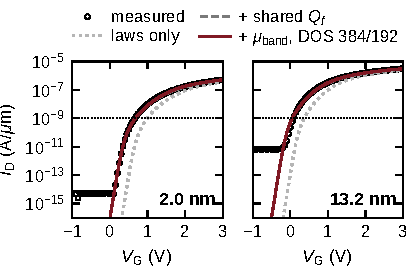
\includegraphics[width=\linewidth]{04_calibration}
      \src{V1 chain at drain bias 0.7\,V: laws only (runs 0001, 0002); + shared $Q_f$ (0003, 0004); final (0038,
        0040: tail-DOS quadrature 384/192, physical deck, band mobility scaled exactly to the measured on-current).
        \fourData\sref{Januar2026}.}
    \end{column}
    \begin{column}{0.47\textwidth}
      {\scriptsize
      \setlength{\tabcolsep}{3pt}
      \renewcommand{\arraystretch}{1.1}
      \begin{tabular}{@{}lcc@{}}
        \toprule
        2.0 / 13.2\,nm & V1 & V2 \\
        \midrule
        Shared $Q_f$ ($10^{12}$\cmsq) & 1.73 & 1.38 \\
        $\mu_\mathrm{band}$ (\cmVs) & 17.69 / 61.60 & 17.54 / 63.21 \\
        $\Delta\Vthcc$ vs measured (mV) & $+19$ / $-29$ & $+6$ / $+21$ \\
        Active RMSE (dec) & 0.043 / 0.081 & 0.065 / 0.097 \\
        \bottomrule
      \end{tabular}\par}
      \src{V1: confinement law fitted to published slab DFT; V2: laws fitted to this work's DFT. On-current exact in
        both; measured $\Vthcc$ 0.662 / 0.083\,V. All rows \fourSrcLab{fitted} (C013).}
      \begin{itemize}\footnotesize
        \item $Q_f$ shifts the curve rigidly (verified to 1\,mV) and $\Id \propto \mu_\mathrm{band}$: one shared
          $Q_f$ sets the threshold pair, $\mu_\mathrm{band}$ each on-current \lab{computed}
        \item 6.3\,nm needs its own $Q_f = 8.7\times10^{10}$\cmsq{} and its own $\mu_\mathrm{band}$ \lab{fitted};
          even then its late, steep turn-on is not reproduced \lab{computed}
      \end{itemize}
    \end{column}
  \end{columns}
  \takeaway{Agreement at the anchors is a calibration, not a test of the thickness laws.}
\end{frame}

% ---------------------------------------------------------------------------------------------------------------------
\begin{frame}[t]{The shared tail fits the deep swing, not every window}
  \fourTop
  {\footnotesize
  \setlength{\tabcolsep}{4pt}
  \renewcommand{\arraystretch}{1.05}
  \begin{tabular*}{\textwidth}{@{}l@{\extracolsep{\fill}}cccl@{}}
    \toprule
    Window & 2.0\,nm & 6.3\,nm & 13.2\,nm & \\
    \midrule
    $10^{-11}$--$10^{-10}$\,\fourAum, meas.\ / sim. & 121.2 / 123.5 & 124.5 / 124.5 & 91.8$^{\ast}$ / 90.9 &
      \lab{fitted} \\
    $(2.15$--$21.5)\times10^{-5}\,I_\mathrm{on}$, meas.\ / sim. & $123.6\pm1.0$ / 126.4 & $122.7\pm9.3$ / 121.3 &
      $115.3\pm2.4$ / 131.3 & \lab{computed}\fourC{C008} \\
    $10^{-10}$--$10^{-9}$\,\fourAum, sim.\ $-$ meas. & $+20$ & $+6$ & $+25$ & \lab{computed} \\
    \bottomrule
  \end{tabular*}\par}
  \src{Swing in mV/dec. V1 calibrated model; the 6.3\,nm curve with its own $Q_f$ and band mobility. $^{\ast}$After
    subtracting the off-state floor (two points); raw 136.1\,mV/dec. Middle row: the normalised window (amendment A1 of
    the extraction protocol). \fourData\sref{Januar2026}.}
  \begin{itemize}\small
    \item One shared $W_\mathrm{TA} = 40$\,meV matches the deepest window within 2.3\,mV/dec at 2.0 and 6.3\,nm
      \lab{fitted}; at 13.2\,nm only after floor subtraction, so it is not claimed there
    \item In the normalised window the 13.2\,nm simulation is $16\pm3$\,mV/dec too high: reported as a finding, not
      tuned away \lab{computed}\fourC{C010}
    \item Above $10^{-10}$\,\fourAum{} the model is too soft in every film: tail filling holds, the V1 tail shape
      does not \lab{inferred}
  \end{itemize}
  \takeaway{Tail filling sets the swing in all films; the V1 tail shape is too soft above $10^{-10}$\,\fourAum.}
\end{frame}

% ---------------------------------------------------------------------------------------------------------------------
\begin{frame}[t]{Every out-of-sample 6.3\,nm threshold prediction failed}
  \fourTop
  \begin{columns}[T,onlytextwidth]
    \begin{column}{0.50\textwidth}
      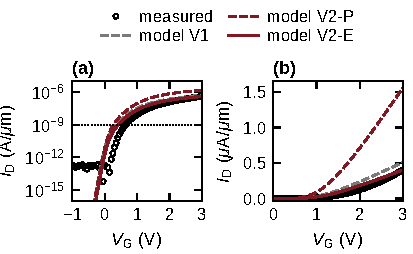
\includegraphics[width=\linewidth]{04_holdout}
      \src{6.3\,nm threshold held out (no $Q_f$ fitted to it). V1 (run 0014) uses the band mobility of the V0 fit of
        this curve, 12.4\cmVs: threshold-only test. V2 (run 0060): P from the registered rule $\propto t^{0.675}$,
        38.39\cmVs; E scaled by 0.2579 to the measured on-current. \fourData\sref{Januar2026}.}
    \end{column}
    \begin{column}{0.47\textwidth}
      \vspace{-1mm}
      {\scriptsize
      \setlength{\tabcolsep}{4pt}
      \renewcommand{\arraystretch}{1.05}
      \begin{tabular}{@{}lcc@{}}
        \toprule
        Prediction (run) & $\Vthcc$ (V) & Miss (V) \\
        \midrule
        V1, shared laws (0014) & 0.350 & \textbf{\textminus0.29} \\
        V2-P, predicted $\mu$ (0060) & 0.270 & \textbf{\textminus0.37} \\
        V2-E, $\mu$ scaled to $I_\mathrm{on}$ (0060) & 0.417 & \textbf{\textminus0.23} \\
        \bottomrule
      \end{tabular}\par}
      \src{Measured 0.644\,V; pass required $|\Delta\Vthcc| \le 0.10$\,V: all three \fourSrcLab{falsified} (C014). V2 registered in commit
        7b75ee6, on-state correction a914165 before the result. The registered T2 anchor check failed at 2.0\,nm (RMSE,
        by 0.001\,dec).}
      \begin{itemize}\footnotesize\setlength{\itemsep}{1pt}
        \item ATLAS matched the registered T3 thresholds within 0.3\,mV \lab{computed}
        \item DFT laws shrink the miss by only about 0.04\,V; the linear threshold is 0.58\,V too low; rule P gives
          four times $I_\mathrm{on}$ \lab{computed}
        \item The computed $\dEc$ law, applied rigidly, gives $-0.21$ to $-0.22$\,V from 2.0 to 6.3\,nm; measured
          $-0.018$\,V \lab{derived}
      \end{itemize}
    \end{column}
  \end{columns}
  \takeaway{The model describes the anchor films; it does not predict the thickness dependence.}
\end{frame}

% ---------------------------------------------------------------------------------------------------------------------
\begin{frame}[t]{One transfer curve fixes combinations, not parameters}
  \fourTop
  \begin{columns}[T,onlytextwidth]
    \begin{column}{0.53\textwidth}
      {\scriptsize
      \setlength{\tabcolsep}{4pt}
      \renewcommand{\arraystretch}{1.2}
      \begin{tabular}{@{}lrrl@{}}
        \toprule
        Change at 2.0\,nm & $\Delta\Vthcc$ (V) & $\Delta$SS (mV/dec) & Action \\
        \midrule
        Gate WF $+0.1$\,eV & $+0.100$ & 0 & rigid \\
        $\chi$ $-0.1$ / $+0.1$\,eV & $+0.100$ / $-0.100$ & 0 & rigid \\
        Confinement off & $-0.316$ & $+15.3$ & near-rigid \\
        $N_t\times1.5$ & $+0.082$ & $+49.0$ & slope, delay \\
        $m^{*}\times1.3$ (via $\fourNc$) & $-0.044$ & $-18.0$ & slope \\
        $W_\mathrm{TA}$ $+5$\,meV & $+0.020$ & $+4.6$ & slope \\
        $D_\mathrm{it}\times3$ & $+0.025$ & -- & small shift \\
        $N_D\times2$ & $-0.009$ & -- & negligible \\
        $\varepsilon_\mathrm{IWO} = 10.55$ & $-0.001$ & -- & negligible \\
        \bottomrule
      \end{tabular}\par}
      \src{One-at-a-time ATLAS pairs \fourSrcLab{computed} (runs 0048, 0020/0021, 0016, 0023, 0050, 0024, 0025, 0022,
        0026); SS over $10^{-10}$--$10^{-9}$\,A/\textmu m. On-current change: $-25.1$\,\% for $N_t\times1.5$,
        $+21.4$\,\% for confinement off. No Jacobian or profile analysis was made.}
    \end{column}
    \begin{column}{0.44\textwidth}
      \begin{itemize}\footnotesize
        \item Work function, affinity, uniform fixed charge and confinement shift act as one number per film:
          $\dEc(2\,\mathrm{nm}) = 0.353$\,eV $\equiv 1.97\times10^{12}$\cmsq{} of fixed charge
          \lab{computed}\fourC{C018}
        \item $\mu_\mathrm{band}$ trades with $N_t$: on $I_\mathrm{on}$, $N_t\times1.5 \equiv \mu\times1.33$; series
          resistance trades with the tail exponent \lab{derived}\fourC{C018}
        \item One shared offset fits the three thresholds equally well with and without confinement: rms 0.136 vs
          0.133\,V \lab{computed}
        \item Separating them needs C--V flat band against $t$, the optical gap, gated Hall and a transfer-length
          series
      \end{itemize}
    \end{column}
  \end{columns}
  \takeaway{The calibrated set is one member of a family of equivalent calibrations, not an extraction.}
\end{frame}

% ---------------------------------------------------------------------------------------------------------------------
\begin{frame}[t]{Thickness-independent contacts cannot create the trend}
  \fourTop
  \begin{columns}[T,onlytextwidth]
    \begin{column}{0.38\textwidth}
      \centering
      \vspace{2mm}
      \begin{tikzpicture}[x=0.80mm,y=1.2mm,line width=0.5pt,font=\footnotesize]
        % circuit: source - R_S - channel - R_D - drain
        \draw (0,10) -- (6,10);
        \draw (6,8) rectangle (14,12); \node[above] at (10,12) {$R_\mathrm{S}$};
        \draw (14,10) -- (19,10);
        \draw[ntumaroon] (19,7.5) rectangle (35,12.5); \node at (27,10) {$R_\mathrm{ch}(\Vg)$};
        \draw (35,10) -- (40,10);
        \draw (40,8) rectangle (48,12); \node[above] at (44,12) {$R_\mathrm{D}$};
        \draw (48,10) -- (54,10);
        \fill (0,10) circle[radius=0.7mm]; \fill (54,10) circle[radius=0.7mm];
        \node[left] at (-0.5,10) {S}; \node[right] at (54.5,10) {D};
        \draw[{Latex[length=1.5mm]}-{Latex[length=1.5mm]}] (0,19) -- (54,19);
        \node[fill=white,inner sep=1pt] at (27,19) {$\Vd = 0.7$\,V};
        % voltage share required at 2.0 nm (hypothetical)
        \fill[black!25] (0,0) rectangle (22.4,3.5);
        \fill[black!25] (31.6,0) rectangle (54,3.5);
        \draw (0,0) rectangle (54,3.5);
        \draw (22.4,0) -- (22.4,3.5); \draw (31.6,0) -- (31.6,3.5);
        \node[below,align=center,text width=44mm,font=\scriptsize] at (27,-0.8) {required at 2.0\,nm: 83\,\% of
          $\Vd$ across the contacts (grey), 17\,\% across the channel};
      \end{tikzpicture}
      \src{Schematic; the split is the hypothetical needed for contacts alone to cause the 2.0\,nm deficit.}
    \end{column}
    \begin{column}{0.59\textwidth}
      \begin{itemize}\footnotesize
        \item Contacts alone would need $R_\mathrm{sd}W \approx 1.15\times10^{6}\,\Omega\,\si{\micro\metre}$ at
          2.0\,nm: $\rho_c \approx 0.26\,\Omega\,\mathrm{cm^2}$, $L_T \approx 45\,\si{\micro\metre}$ \lab{derived}
        \item That drops 83\,\% of $\Vd$ in the contacts; per contact (about 570\,$\Omega$\,mm) it is about 5700
          times the contact resistance of related metal/\InO{} contacts, below 0.1\,$\Omega$\,mm\sref[p.~167]{Si2022}
        \item Wrong sign: $\theta_\mathrm{net} = -0.10$ / $-0.12$ / $-0.046$\,V$^{-1}$ (2.0 / 6.3 / 13.2\,nm);
          series resistance needs the opposite sign \lab{derived}
        \item Wrong direction: at fixed $\rho_c$ the contact share scales as $R_\mathrm{sh}^{-1/2}$, so a common
          contact penalises the thick film \lab{derived}\fourC{C019}
        \item Inside the calibrated trap model: $R_\mathrm{sd}W \lesssim 5\times10^{4}\,\Omega\,\si{\micro\metre}$
          ($\le 4$\,\%) at 2.0\,nm, $\lesssim$ 1--2$\times10^{4}\,\Omega\,\si{\micro\metre}$ (4--9\,\%) at
          13.2\,nm \lab{fitted}
      \end{itemize}
    \end{column}
  \end{columns}
  \takeaway{Contacts do not make the trend; a minor share needs a transfer-length series to settle.}
\end{frame}

% ---------------------------------------------------------------------------------------------------------------------
\begin{frame}[t]{Campaign C10 tests one parameter set shared by all three films}
  \fourTop
  \begin{columns}[T,onlytextwidth]
    \begin{column}{0.50\textwidth}
      \begin{itemize}\footnotesize
        \item Five shared fitted parameters: offset $\Delta V_0$ (via $Q_f$), $\mu_\infty$, length $\ell$, tail sheet
          $N_s$ ($N_t = N_s/t$), $W_\mathrm{TA}$; no per-film charge or mobility; DFT laws in $\chi$, $\Eg$, $\fourNc$,
          $\mu$
      \end{itemize}
      {\footnotesize\fourEqSkip
      \[ \mu_\mathrm{band}(t) = \mu_\infty\,\frac{0.208\,\mzero}{m^{*}(t)}\,\frac{1}{1+\ell/t}
         \Big(1-\frac{0.287\,\mathrm{nm}}{t}\Big)^{2} \]
      where $m^{*}(t) = 0.208\,\mzero + \Delta m^{*}(t)$ (DFT increment) and the last factor is the existing roughness
      term.\par}
      \begin{itemize}\footnotesize
        \item The mass ratio gives only $\times0.83$ from 13.2 to 2.0\,nm, about 14\,\% of the logarithmic drop the
          calibrated models need \lab{derived}; by design $\ell$ carries the rest (H-D, sealed)
        \item $\Delta V_0$, $\mu_\infty$, $\ell$ are profiled offline by exact transformations; three degrees of
          freedom remain
        \item Acceptance, stop rules and the expected 6.3\,nm failure were fixed before any launch
      \end{itemize}
    \end{column}
    \begin{column}{0.47\textwidth}
      {\scriptsize
      \setlength{\tabcolsep}{3pt}
      \renewcommand{\arraystretch}{1.08}
      \begin{tabularx}{\linewidth}{@{}l r>{\raggedright\arraybackslash}X@{}}
        \toprule
        Stage & Launches & Content \\
        \midrule
        S0 smoke & 2 & 2.0\,nm baseline; gate tunnelling \\
        S1 baselines & 7 & baselines; numerics; 3-D $\fourNc$ \\
        \midrule
        S2 off-state floor & 17 & generation; leakage; ungated strip \\
        S3 model form & 27 & confinement off; branches \\
        S4 calibration & 69 & space-filling and adaptive \\
        S5 leave-one-out & 30 & held-out film never tuned \\
        S6 sensitivity & 27 & DFT low/high; mass; $N_D$; traps \\
        S7 31.8\,nm & 2 & frozen model, never fitted \\
        \midrule
        Reserve & 19 & total 200 \\
        \bottomrule
      \end{tabularx}\par}
      \src{Planned launches, approved 10 Oct 2026 (D-13); regenerated matrix: 184 + 16 reserve (recorded
        inconsistency). S0/S1 used 14 launches (S0-02 needed six), seen before the register freeze; 17 of 200 used by
        14 Oct.}
    \end{column}
  \end{columns}
  \takeaway{With one offset for all three films, the first-principles inputs can fail for the first time.}
\end{frame}

% ---------------------------------------------------------------------------------------------------------------------
\begin{frame}[t]{The $\fourNc$ convention alone moves the 2.0\,nm threshold by 142\,mV}
  \fourTop
  \begin{columns}[T,onlytextwidth]
    \begin{column}{0.57\textwidth}
      {\scriptsize
      \setlength{\tabcolsep}{3pt}
      \renewcommand{\arraystretch}{1.05}
      \begin{tabularx}{\linewidth}{@{}l>{\raggedright\arraybackslash}p{3.05cm}>{\raggedright\arraybackslash}X@{}}
        \toprule
        Run & Test & Result \\
        \midrule
        S1-01 & 6.3\,nm baseline & RMSE 1.18\,dec; $\Id(3\,\mathrm{V})$ $\times4.87$ \\
        S1-02 & 13.2\,nm baseline & RMSE 0.056\,dec \\
        S1-03 & 13.2\,nm, mesh $\times0.7$ & pass, $\Delta$RMSE $-0.0005$\,dec \\
        S1-04 & 2.0\,nm, DOS quadrature $\times2$ & pass, $\Delta$RMSE $-0.00002$\,dec \\
        S1-05 & 2.0\,nm, 3-D instead of quasi-2-D $\fourNc$ & $\Delta\Vthcc$ $+142$\,mV vs registered $+40$ to
          $+70$\,mV: \textbf{failed}; $\Delta$SS $+49$\,mV/dec; RMSE $0.367\to0.053$\,dec \\
        \bottomrule
      \end{tabularx}\par}
      \src{Stage S1 (runs 0061--0074 with S0), seen before register revision 2; model-internal, at the shared start
        parameters \fourSrcLab{computed}. $\Id(3\,\mathrm{V})$ relative to the measured value. S1-06 (13.2\,nm, two carriers) timed out: unresolved. S1-07 (ATLAS check of the
        offline profiling) passed, $\le 2.05\times10^{-4}$\,dec.}
      \begin{itemize}\footnotesize
        \item Quasi-2-D $\fourNc$ at 2.0\,nm: within 0.86\,mV of true 2-D statistics at threshold, $I_\mathrm{on}$
          about 7--8\,\% high \lab{inferred}
        \item $\fourNc$ is degenerate with $Q_f$ and trap densities: each fitted value must name its convention
          \lab{inferred}
      \end{itemize}
    \end{column}
    \begin{column}{0.40\textwidth}
      \centering
      \begin{tikzpicture}[x=0.32mm,y=1mm,font=\scriptsize]
        \fill[black!15] (40,0) rectangle (70,4);
        \draw[line width=0.5pt] (0,0) -- (160,0);
        \foreach \x in {0,40,80,120,160} {\draw (\x,0) -- (\x,-1.2); \node[below] at (\x,-1.2) {\x};}
        \node[above] at (55,4) {registered $+40$ to $+70$};
        \fill[ntumaroon] (142,2) circle[radius=0.8mm];
        \node[above,text=ntumaroon] at (142,3.5) {S1-05: $+142$};
        \node[below] at (80,-5.5) {$\Delta\Vthcc$ at 2.0\,nm (mV)};
      \end{tikzpicture}
      \src{Registered expectation (register revision 1) and run S1-05.}
      \begin{itemize}\footnotesize
        \item Audit A13: no implementation error; of the $+142$\,mV, $+37.5$\,mV from the statistics and
          $+89.5$\,mV from extra charge in the 40\,meV tail (127\,mV itemised) \lab{computed}
        \item The effective slope factor at $10^{-9}$\,\fourAum{} is about 3.5, not the 1.47 assumed in the
          registration \lab{computed}
      \end{itemize}
    \end{column}
  \end{columns}
  \takeaway{The DOS convention alone moves $\Vthcc$ by a third to two thirds of a 6.3\,nm miss.}
\end{frame}

% ---------------------------------------------------------------------------------------------------------------------
\begin{frame}[t]{Sealed stages S2--S7 decide transfer, not device physics}
  \fourTop
  \begin{center}
    \begin{minipage}{0.86\textwidth}
      \sealed{Outcomes of stages S2--S7 of campaign C10 (every launch after the register freeze of 10 Oct 2026)}
    \end{minipage}
  \end{center}
  \vspace{4mm}
  \begin{columns}[T,onlytextwidth]
    \begin{column}{0.56\textwidth}
      {\scriptsize
      \setlength{\tabcolsep}{3pt}
      \renewcommand{\arraystretch}{1.05}
      \begin{tabularx}{\linewidth}{@{}l>{\raggedright\arraybackslash}X l@{}}
        \toprule
        Stage & Question it will decide & Register \\
        \midrule
        S2 & can gate leakage, generation or an ungated strip give the off-state floors? & H-A, H-B, H-C \\
        S3 & how much threshold the first-principles inputs carry (all off) & H-E \\
        S4 & is a $1/t$ scattering term needed in the band mobility? & H-D \\
        S4, S5 & does one set transfer to each held-out film; what remains at 6.3\,nm? & H-F, H-J \\
        S6, S7 & sensitivity to the inputs; 31.8\,nm with the frozen model, never fitted & -- \\
        \bottomrule
      \end{tabularx}\par}
      \src{Registered predictions: Part 3. Stage-to-hypothesis assignment ours, from the stage contents. Stop rule: if
        after the first calibration sub-stage the best shared fit exceeds 0.30\,dec rms log-current error with
        systematic 6.3\,nm residuals, the shared model is reported as failed, with no per-film rescue.}
    \end{column}
    \begin{column}{0.41\textwidth}
      {\small\textbf{What C10 cannot establish}\par}
      \begin{itemize}\small
        \item The device physics: four single-device curves, one $\Vd$ and no gate current leave several mechanisms
          indistinguishable
        \item Confinement: not identifiable from transfer curves\fourC{C018}
        \item Success on all three films would still be a calibration
      \end{itemize}
    \end{column}
  \end{columns}
  \takeaway{Decisive next step: replicate devices, C--V and the optical gap versus thickness.}
\end{frame}

% 05_dft_methods.tex -- Part 5, first-principles methods. Sources: research_monograph/chapters/M04_dft_theory.tex
% (Born-Oppenheimer, Kohn-Sham, PBE gap problem, HSE06, smearing), M04b_dft_numerics.tex (plane waves and N_pw table,
% PAW band counting and correction X1, SCF force error and correction V1, relaxation, slabs, dipole, two-step
% alignment), 13_dft_rev.tex (methods: data sets, convergence stage, k grids, slab recipe and symmetry, vacuum test,
% codes, GPU check, settings table incl. nbnd 190, band projections of the 1 nm W film), M10_w_and_vacancies.tex (W and
% H-L cell settings); evidence/FACT_REGISTRY.tsv (FACT-001, 002, 014, 019, 031, 042, 045);
% appendices/MG_corrections.tex (X1, X4, V1, V2); cern_htcondor/results/RESULTS_LOG.md (H-L settings: Gaussian 0.005 Ry,
% conv_thr 1e-8; 2 nm W film conv_thr 1e-8); ledger C035 (force-only check). Raw outputs read for checks:
% bulk_In2O3_protocol/vcrelax_ecut71_k3.out (nbnd 190), slab1r_final_cpu/scf.out (5 746 731 G-vectors),
% slab2_relax_c2/scf.out (82.10 GB), iwo_W8b/scf_k4.out and iwo_slab1_final_cpu/scf.out (printed MV occupations).
% MV convention: the slide uses the weight as Quantum ESPRESSO applies it, f = 1/2 erfc(u) + exp(-u^2)/sqrt(2 pi),
% u = (eps - mu)/sigma + 1/sqrt2, which reproduces every printed occupation of the W cells to 3e-4 (max printed 1.0738,
% none negative). Monograph eq. mono-dft-mv and the M04b key result ("MV weights can be negative") give the mirror image
% 1 - f(-x) and are flagged for an erratum; the slide does not repeat them.
% Figures: tools/fig_05_dft_methods.py (data: qe_workflow/analysis_2026-10-13_full/out/f01_bulk_convergence.json,
% f03_bulk_alignment.json, cern_htcondor/results/slab2_relax_c2/slab2_relax_c2_avg.dat, iwo_W8b/scf_k4.out).
% Blind rules: only protocol facts and force-only checks (C035) of the amorphous campaign appear; no electronic quantity
% of any amorphous cell.
% Note: frame bodies start with a command, never with a brace group (beamer would read a subtitle).
\providecommand{\fiveVV}{\bar{\bar{V}}}
% denser slides: footnotesize bullets, local to the frame in which it is called
\providecommand{\fivedense}{\setbeamerfont{itemize/enumerate body}{size=\footnotesize}%
  \setbeamerfont{itemize/enumerate subbody}{size=\footnotesize}}
% pull the frame body up to the title rule (frames are top-aligned, as in sections 02, 04, 10, 12-14)
\providecommand{\fiveTop}{\vspace{-2.5mm}}
% evidence label inside a \src line (inherits the \tiny grey source text instead of the larger \lab size)
\providecommand{\fivesrclab}[1]{[\textsc{\MakeLowercase{#1}}]}

\partslide{Part 5}{First-principles methods}

% ---------------------------------------------------------------------------------------------------------------------
\begin{frame}[t]{PBE gives the geometries; only gap differences are trusted}
  \fivedense\fiveTop
  \begin{columns}[T,onlytextwidth]
    \begin{column}{0.50\textwidth}
      \begingroup\footnotesize\textbf{Kohn--Sham DFT and the gap}\srefs{Hohenberg1964,Kohn1965,PerdewLevy1983,ShamSchluter1983}\par\endgroup
      \vspace{-3mm}
      \begingroup\footnotesize
      \begin{gather*}
        \Big[-\tfrac12\nabla^2 + v_{\mathrm{ext}} + v_{\mathrm{H}}[n] + v_{\mathrm{xc}}[n]\Big]\psi_j = \varepsilon_j\psi_j ,
        \quad n = \textstyle\sum_j f_j|\psi_j|^2 \\
        \Eg = \Eg^{\mathrm{KS}} + \Delta_{\mathrm{xc}}, \qquad \Delta_{\mathrm{xc}} = 0 \text{ in PBE}
      \end{gather*}\par\endgroup
      \vspace{-1.5mm}
      \begingroup\scriptsize\color{inkgrey}Hartree units. $v_{\mathrm{ext}}, v_{\mathrm{H}}, v_{\mathrm{xc}}$: nuclear,
        Hartree and exchange--correlation potentials; $f_j$: occupations; $\Delta_{\mathrm{xc}}$: jump of the exact
        $v_{\mathrm{xc}}$ at integer electron number.\par\endgroup
      \vspace{1mm}
      \begingroup\footnotesize Born--Oppenheimer, static lattice\sref{Born1927}: fixed nuclei; corrections in powers
        of $\kappa = (m_e/M)^{1/4}$, 0.076 (O) and 0.047 (In) \lab{derived}: vibrations at order $\kappa^2$,
        non-adiabatic terms higher (not estimated).\par\endgroup
    \end{column}
    \begin{column}{0.46\textwidth}
      \begin{itemize}
        \item PBE\sref{Perdew1996} for all relaxations and production runs. Bulk gap 0.8887\,eV \lab{computed};
          measured 2.7--2.9\,eV\srefs{Walsh2008,Irmscher2014}.
        \item HSE06\srefs{Heyd2003,Heyd2006,Krukau2006}: a fraction $\alpha = 0.25$ of the short-range exchange is
          exact, $\omega = 0.106$\,bohr$^{-1}$; fixed PBE geometry. Bulk gap 2.108\,eV (norm-conserving,
          $\Gamma$-only $q$; 41.8\,meV lower with $3\times3\times3$ $q$) \lab{computed}.
        \item Not included: zero-point renormalisation, spin--orbit coupling, spin polarisation (production
          runs) \lab{assumed}.
      \end{itemize}
    \end{column}
  \end{columns}
  \takeaway{No absolute PBE gap is used; only film-minus-bulk shifts, checked with HSE06 at 1\,nm.}
\end{frame}

% ---------------------------------------------------------------------------------------------------------------------
\begin{frame}[t]{A 71/568\,Ry basis met the criteria fixed before the runs}
  \fivedense\fiveTop
  \begin{columns}[T,onlytextwidth]
    \begin{column}{0.45\textwidth}
      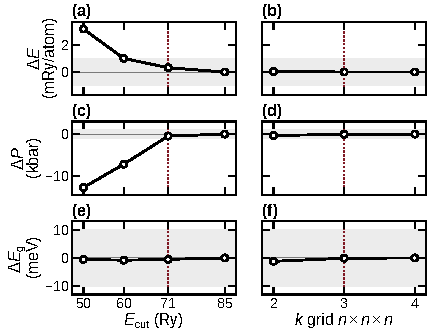
\includegraphics[width=0.93\linewidth]{05_convergence}
      \src{Bulk \InO{} (40-atom primitive cell at the experimental $a = 10.117$\,\AA{}), PAW-PBE: change against
        85\,Ry (left) and 4$\times$4$\times$4 (right). Grey: criteria; dotted: settings used (71\,Ry,
        3$\times$3$\times$3). This work \fivesrclab{computed}.}
    \end{column}
    \begin{column}{0.51\textwidth}
      \begin{itemize}
        \item Criteria (protocol of 26 Sep 2026): the next step may change the energy by $<1$\,mRy/atom, the pressure
          by $<1$\,kbar, the gap by $<10$\,meV.
        \item 71\,Ry is the lowest cutoff that passes: 0.32\,mRy/atom, 0.47\,kbar and 0.5\,meV against 85\,Ry
          \lab{computed}. PAW density cutoff: $8E_{\mathrm{cut}} = 568$\,Ry.
        \item Monkhorst--Pack grids\sref{Monkhorst1976}: 2$\times$2$\times$2 already passes; used: 3$\times$3$\times$3
          (bulk), 3$\times$3$\times$1 (slabs), 4$\times$4$\times$4 (80-atom W and H-L single points).
        \item Quantum ESPRESSO 7.5 on CPUs\srefs{Giannozzi2009,Giannozzi2017}, NVIDIA GPU build
          7.3.1\sref[NGC container \texttt{hpc/quantum\_espresso:qe-7.3.1}]{NvidiaQE}: the same input gives energies
          $5\times10^{-7}$\,Ry apart \lab{computed}.
      \end{itemize}
    \end{column}
  \end{columns}
\end{frame}

% ---------------------------------------------------------------------------------------------------------------------
\begin{frame}[t]{Plane-wave counts follow the volume law to within 0.15\,\%}
  \fivedense\fiveTop
  \begin{columns}[T,onlytextwidth]
    \begin{column}{0.57\textwidth}
      \vspace*{-0.5\abovedisplayskip}
      \begingroup\footnotesize
      \[
        N_{\mathrm{pw}} \approx \frac{4\pi k_c^3/3}{(2\pi)^3/\Omega} = \frac{\Omega\,E_{\mathrm{cut}}^{3/2}}{6\pi^2},
        \qquad k_c = E_{\mathrm{cut}}^{1/2}
      \]\par\endgroup
      \vspace{-0.3mm}
      \begingroup\scriptsize\color{inkgrey}$\Omega$: cell volume (bohr$^3$); $E_{\mathrm{cut}}$ in Ry; plane waves with
        $|\mathbf{k}+\mathbf{G}|^2 \le E_{\mathrm{cut}}$; $N_b$: number of bands.\par\endgroup
      \vspace{2mm}
      \begingroup\scriptsize
      \renewcommand{\arraystretch}{1.1}\setlength{\tabcolsep}{5.5pt}
      \begin{tabular}{@{}l r r r r@{}}
        \toprule
        Cell (atoms) & $\Omega$ (bohr$^3$) & formula & printed & bands \\
        \midrule
        bulk In$_{16}$O$_{24}$ (40, primitive) & 3\,693.6 & 37\,315 & 37\,359 & 190 \\
        bulk In$_{31}$WO$_{48}$ (80) & 7\,387.2 & 74\,630 & 74\,653 & 424 \\
        1\,nm slab In$_{24}$O$_{48}$H$_{24}$ (96) & 25\,140.0 & 253\,982 & 253\,973 & 328 \\
        2\,nm slab In$_{56}$O$_{96}$H$_{24}$ (176) & 32\,429.2 & 327\,622 & 327\,585 & 680 \\
        \bottomrule
      \end{tabular}\par\endgroup
      \src{$E_{\mathrm{cut}} = 71$\,Ry. Printed: plane waves at $\Gamma$ in the \texttt{pw.x} output; bands:
        \texttt{nbnd} of the run. This work \fivesrclab{computed}.}
    \end{column}
    \begin{column}{0.39\textwidth}
      \begin{itemize}
        \item The density sphere at $8E_{\mathrm{cut}}$ holds $8^{3/2} \approx 22.6$ times more components: 5\,746\,731
          for the 1\,nm slab \lab{computed}.
        \item Work per SCF step grows as $N_b^2N_{\mathrm{pw}}$. From 1 to 2\,nm: bands 328 to 680, $N_{\mathrm{pw}}$
          $+29$\,\%, work $\times5.5$ \lab{derived}.
        \item 2\,nm wave functions at one $k$ point: $680\times327\,585\times16$\,B $= 3.6$\,GB \lab{derived};
          \texttt{pw.x} estimates 82\,GB per process for the single-process GPU relaxation \lab{computed}.
      \end{itemize}
    \end{column}
  \end{columns}
  \takeaway{The 176-atom film needed a large-memory GPU or a distributed CPU run.}
\end{frame}

% ---------------------------------------------------------------------------------------------------------------------
\begin{frame}[t]{A W cell has one valence band fewer than the pure cell}
  \fivedense\fiveTop
  \begin{columns}[T,onlytextwidth]
    \begin{column}{0.47\textwidth}
      \begingroup\footnotesize PAW\srefs{Bloechl1994,Kresse1999}, pslibrary 1.0.0 data sets\sref{DalCorso2014}\par\endgroup
      \vspace{0.5mm}
      \begingroup\scriptsize
      \renewcommand{\arraystretch}{1.0}
      \begin{tabular}{@{}l l r l@{}}
        \toprule
        & valence & $Z$ & bands below the gap \\
        \midrule
        In & 4d$^{10}$5s$^2$5p$^1$ & 13 & 5 (In 4d) \\
        W  & 5s$^2$5p$^6$5d$^4$6s$^2$ & 14 & 4 (W 5s, 5p) \\
        O  & 2s$^2$2p$^4$ & 6 & 4 (O 2s, 2p) \\
        H  & 1s$^1$ & 1 & none (O--H within O bands) \\
        \bottomrule
      \end{tabular}\par\endgroup
      \vspace{1.1mm}
      \begingroup\footnotesize\centering
        $N_{\mathrm{VB}} = 5n_{\mathrm{In}} + 4n_{\mathrm{W}} + 4n_{\mathrm{O}}, \qquad
        N_{\mathrm{ex}} = \textstyle\sum Z - 2N_{\mathrm{VB}}$\par\endgroup
      \vspace{0.9mm}
      \begingroup\scriptsize
      \renewcommand{\arraystretch}{1.0}
      \begin{tabular}{@{}l r r r@{}}
        \toprule
        cell & $\sum Z$ & $N_{\mathrm{VB}}$ & $N_{\mathrm{ex}}$ \\
        \midrule
        bulk In$_{32}$O$_{48}$ (80-atom conventional) & 704 & 352 & 0 \\
        bulk In$_{31}$WO$_{48}$ & 705 & 351 & 3 \\
        1\,nm In$_{24}$O$_{48}$H$_{24}$ & 624 & 312 & 0 \\
        1\,nm In$_{23}$WO$_{48}$H$_{24}$ & 625 & 311 & 3 \\
        \bottomrule
      \end{tabular}\par\endgroup
      \src{$Z$: valence charges of the data sets; $\sum Z$ as printed by \texttt{pw.x} \fivesrclab{computed};
        $N_{\mathrm{VB}}$, $N_{\mathrm{ex}}$ \fivesrclab{derived}.}
    \end{column}
    \begin{column}{0.49\textwidth}
      \centering
      \begin{tikzpicture}[x=1mm,y=1mm,line width=0.5pt,font=\scriptsize]
        \node[anchor=south] at (9.5,24.2) {1\,nm In$_{24}$O$_{48}$H$_{24}$};
        \node[anchor=south] at (50.5,24.2) {1\,nm In$_{23}$WO$_{48}$H$_{24}$};
        % pure cell
        \draw (0,0) rectangle (19,8.5);
        \node[align=center] at (9.5,4.25) {bands 1--312\\occupied};
        \draw (0,13) rectangle (19,24);
        \node[align=center] at (9.5,18.5) {bands 313--\\empty};
        % W cell
        \draw (33,0) rectangle (68,8.5);
        \node[align=center] at (50.5,4.25) {bands 1--311\\occupied (valence)};
        \draw (33,13) rectangle (68,24);
        \draw[rulegrey] (33,18.5) -- (68,18.5);
        \node at (50.5,15.75) {312: host CB bottom, 2\,e$^-$};
        \node at (50.5,21.25) {313: W-5d rich, $\approx$1\,e$^-$};
        \node[inkgrey] at (9.5,10.75) {gap};
        \node[inkgrey] at (50.5,10.75) {gap};
        % the misreading of 30 September
        \node[align=center,ntumaroon] (mis) at (26,4.25) {W cell:\\312 read\\as VB top};
        \draw[-{Stealth[length=1.6mm]},ntumaroon,line width=0.7pt] (mis.north) .. controls (26,12.5) and (27.5,15.75) .. (32.6,15.75);
      \end{tikzpicture}
      \vspace{1mm}
      \begin{itemize}
        \item At $\Gamma$: band 311 is O 2p, 313 has 56\,\% W 5d, resonant 1.22\,eV above the host band bottom in
          this film (2\,nm: 1.34\,eV; bulk: 1.76--1.80\,eV), at the computed filling of 3\,e per cell
          \lab{computed}.
      \end{itemize}
    \end{column}
  \end{columns}
  \takeaway{Reading band 312 as the VB top caused the 30 Sep ``W level below CB'' (correction X1).}
\end{frame}

% ---------------------------------------------------------------------------------------------------------------------
\begin{frame}[t]{Marzari--Vanderbilt weights exceed 1 below $\mu$: not occupations}
  \fivedense\fiveTop
  \begin{columns}[T,onlytextwidth]
    \begin{column}{0.42\textwidth}
      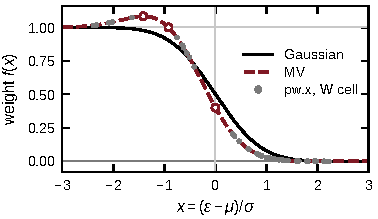
\includegraphics[width=\linewidth]{05_smearing}
      \src{MV as \texttt{pw.x} applies it: $f = \tfrac12\mathrm{erfc}(u) + e^{-u^2}\!/\sqrt{2\pi}$,
        $u = x + 1/\sqrt2$. Circles: 0.40, 1 and 1.083 at $x = 0$, $-0.92$, $-\sqrt2$ \fivesrclab{derived}. Dots: 51
        fractional weights printed by \texttt{pw.x} for a bulk W cell (largest 1.074), within $3\times10^{-4}$ of $f$
        \fivesrclab{computed}.}
    \end{column}
    \begin{column}{0.55\textwidth}
      \begin{itemize}
        \item W cells are metals: weights $f(x)$, $x = (\varepsilon-\mu)/\sigma$; $F = E - \sigma S$ is
          variational\sref{Mermin1965}.
        \item Gaussian $\tfrac12\mathrm{erfc}(x)$ stays in $[0,1]$. Marzari--Vanderbilt (MV)\sref{Marzari1999}: energy
          error $O(\sigma^3)$, but 0.40 at $\mu$ and 1.083 at $\sqrt2\sigma$ below $\mu$ (0.19\,eV at 0.01\,Ry)
          \lab{derived}.
        \item Counts near $\mu$ depend on $\sigma$ and $f$: the W-5d projections (0.09--0.43\,e \lab{computed}) are
          not a W charge.
      \end{itemize}
      \vspace{0.5mm}
      \begingroup\scriptsize
      \begin{tabular}{@{}r r l l@{}}
        \toprule
        $\sigma$ (Ry) & (meV) & $f$ & used for \\
        \midrule
        0.01 & 136 & MV & W cells (site study, films) \\
        0.005 & 68 & Gaussian & H-L cells, with and without W \\
        0.002 & 27 & Gaussian & H-L width check \\
        0.001 & 13.6 & Gaussian & amorphous reference finals \\
        \bottomrule
      \end{tabular}\par\endgroup
      \src{\texttt{pw.x} inputs; this work. For comparison, $\kT = 25.85$\,meV at 300\,K.}
    \end{column}
  \end{columns}
  \takeaway{Shallow occupations need Gaussian smearing well below the energy differences.}
\end{frame}

% ---------------------------------------------------------------------------------------------------------------------
\begin{frame}[t]{Slab band edges are placed on the bulk scale in two steps}
  \fivedense\fiveTop\toggletrue{blx@useprefix}% print "Van de Walle" in the footnote (local to this frame)
  \begin{columns}[T,onlytextwidth]
    \begin{column}{0.42\textwidth}
      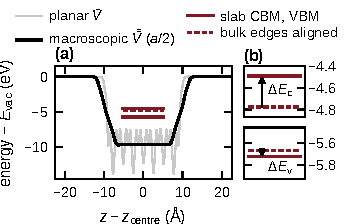
\includegraphics[width=\linewidth]{05_alignment}
      \src{Relaxed 2\,nm (001) slab, PAW-PBE. (a) Ionic plus Hartree potential, planar ($\bar V$) and macroscopic
        ($\fiveVV$) averages; solid: slab edges; dashed: bulk edges via the interior $\fiveVV$. (b) Edges magnified
        (0.47\,eV windows). This work \fivesrclab{computed}.}
    \end{column}
    \begin{column}{0.55\textwidth}
      \begin{itemize}
        \item (001) films, H on surface O that lost In, 25\,\AA{} vacuum\sref[p.~21542]{Lin2022}; 15--35\,\AA{}
          moves EA, IP by $\le 0.1$\,meV \lab{computed}.
        \item Two-step alignment\srefs{VandeWalle1987,Baldereschi1988}; $\fiveVV$: $\bar V$ averaged over $a/2$:
          \[ \dEc = \big(E^{\mathrm{slab}}_{\mathrm{CBM}} - \fiveVV^{\,\mathrm{slab}}_{\mathrm{int}}\big)
                  - \big(E^{\mathrm{bulk}}_{\mathrm{CBM}} - \fiveVV^{\,\mathrm{bulk}}\big) \]
          2\,nm: interior flat within 8\,meV; $\dEc = +0.281$\,eV, $\dEv = -0.054$\,eV \lab{computed}.
        \item 1, 2\,nm: Pcca maps one face onto the other, no dipole \lab{computed}. A sawtooth dipole
          correction\srefs{Neugebauer1992,Bengtsson1999} puts the step in the vacuum; the polar 0.695\,nm film ran
          without it: step 0.44\,V (0.35--0.37\,V if the ramp spans only the vacuum), $\le 0.095$\,eV across the
          film; its effect on the gap is untested \lab{derived}.
      \end{itemize}
    \end{column}
  \end{columns}
  \takeaway{The polar 0.695\,nm film stays out of new primary $\dEc$ fits (correction X4).}
\end{frame}

% ---------------------------------------------------------------------------------------------------------------------
\begin{frame}[t]{SCF force noise is 15 times below the $10^{-3}$\,Ry/bohr threshold}
  \fivedense\fiveTop
  \vspace{-1.8mm}
  \begingroup\scriptsize
  \renewcommand{\arraystretch}{0.95}
  \begin{tabularx}{\textwidth}{@{}l l c c c X@{}}
    \toprule
    Structures & calculation & forces (Ry/bohr) & energy (Ry) & pressure (kbar) & cell degrees of freedom \\
    \midrule
    bulk \InO{} & vc-relax & $10^{-4}$ & $10^{-5}$ & 0.2 & BFGS, all lattice vectors \\
    slabs & vc-relax & $10^{-3}$ & $10^{-4}$ & 0.5 & BFGS, in-plane vectors only \\
    W and H-L cells & relax & $10^{-3}$ & $10^{-4}$ & -- & fixed \\
    \bottomrule
  \end{tabularx}\par\endgroup
  \src{Stopping thresholds. Ions and cell by BFGS, not damped dynamics (correction V2); SCF threshold $10^{-9}$\,Ry ($10^{-8}$\,Ry: metallic
    2\,nm W film, six H-L cells). \texttt{pw.x} inputs; this work.}
  \vspace{-1.5mm}
  \begin{columns}[T,onlytextwidth]
    \begin{column}{0.49\textwidth}
      \begin{itemize}
        \item BFGS\sref{Billeter2003} steps along $-\mathbf{H}^{-1}\nabla E$ ($\mathbf{H}$: approximate Hessian).
          Bulk: 11 steps to $a = 10.306$\,\AA, 1.87\,\% above experiment\sref{Marezio1966} \lab{computed}.
        \item The criterion is per component: the relaxed 1\,nm slab has a norm of $6.1\times10^{-3}$\,Ry/bohr over
          288 components, typically $3.6\times10^{-4}$ \lab{derived}.
        \item \texttt{pw.x} writes coordinates even after a failed BFGS run; amorphous chains need ``bfgs
          converged'' (amendment A19).
      \end{itemize}
    \end{column}
    \begin{column}{0.49\textwidth}
      \begin{itemize}
        \item SCF error $\delta n$: energy error second order, force error first order:
          $\delta F \propto \sqrt{\smash[b]{\texttt{conv\_thr}}}$.
        \item Amorphous 1.0\,nm cell, 134 atoms (force-only check C035), \texttt{conv\_thr} $10^{-7}$\,Ry: SCF force
          correction (norm) $1.3\times10^{-3}$\,Ry/bohr \lab{computed}.
        \item Per component: $1.3\times10^{-3}/\sqrt{402} \approx 6\times10^{-5}$\,Ry/bohr, 15 times below
          $10^{-3}$\,Ry/bohr (correction V1) \lab{derived}.
      \end{itemize}
    \end{column}
  \end{columns}
  \takeaway{Force differences below $10^{-4}$\,Ry/bohr per component need tighter SCF thresholds.}
\end{frame}

% 06_confinement.tex -- Part 6, quantum confinement of crystalline In2O3 films. Sources: research_monograph/chapters/
% M05_confinement_theory.tex (envelope, Kane, finite barrier V4, partition V3, HSE ratio, subband spacing),
% M09_masses_parameters.tex (tab:mono-mass-laws, HSE-corrected gaps), 13_dft_rev.tex (stages 4b, 4c, 5;
% tab:dft-hse, tab:dft-partition, sec:mono-dft-thin), evidence/FACT_REGISTRY.tsv (FACT-002, 010*, 011*, 012-025,
% 028-032), evidence/derived/confinement_analysis.json, appendices/MG_corrections.tex (V3, V4).
% Figures: tools/fig_06_confinement.py (data: qe_workflow/analysis_2026-10-13_full/bands_masses/out/b03_gaps_laws.json,
% evidence/derived/confinement_analysis.json, tables/THICKNESS_LAW_EVIDENCE.csv for the gaps of Lin et al.).
% Note: frame bodies start with a command, never with a brace group (beamer would read a subtitle).
% Naming: "C10" is the frozen device-model law of campaign C10 (the monograph's "V3/C10" law); "V1" is the first device
% model (Part 4). The correction IDs V3/V4 of MG_corrections are not used on the slides.
\partslide{Part 6}{Quantum confinement of crystalline \InO{} films}

% denser slides: footnotesize bullets, local to the frame in which it is called
\providecommand{\sixdense}{\setbeamerfont{itemize/enumerate body}{size=\footnotesize}%
  \setbeamerfont{itemize/enumerate subbody}{size=\footnotesize}}
% evidence label inside a \src line: same wording as \lab, but keeps the small size of the source line
\providecommand{\sixlab}[1]{{\color{inkgrey}[\textsc{\MakeLowercase{#1}}]}}

% ---------------------------------------------------------------------------------------------------------------------
\begin{frame}{Four relaxed films; the two thinnest are special cases}
  \sixdense
  \begin{columns}[T,onlytextwidth]
    \begin{column}{0.59\textwidth}
      \begingroup\scriptsize
      \renewcommand{\arraystretch}{1.05}
      \setlength{\tabcolsep}{4pt}
      \begin{tabular}{@{}l l l c c >{\raggedright\arraybackslash}p{19mm}@{}}
        \toprule
        name & $\tHH$ (nm) & cell & $\Eg$ (eV) & $\dEg$ (eV) & role \\
        \midrule
        0.51\,nm & 0.461 & In$_8$(OH)$_{24}$ & 3.140 & $+2.251$ & excluded \\
        0.75\,nm & 0.695 & In$_{16}$O$_{36}$H$_{24}$ & 2.199 & $+1.310$ & polar; $\dEg$, $\Delta m$, frozen C10 $\dEc$ \\
        1\,nm & 0.930 & In$_{24}$O$_{48}$H$_{24}$ & 1.789 & $+0.900$ & all laws \\
        2\,nm & 1.962 & In$_{56}$O$_{96}$H$_{24}$ & 1.224 & $+0.335$ & all laws \\
        \bottomrule
      \end{tabular}\par\endgroup
      \src{Name: nominal thickness, used in the text; $\tHH$: relaxed H--H thickness. Recipe of Lin
        et al.\sref[p.~21542]{Lin2022}, relaxed; PAW-PBE; bulk gap 0.8887\,eV. This work \sixlab{computed}.}
      \begin{itemize}
        \item 0.461\,nm, one cation plane: all O bonded to H \lab{computed}.
        \item 0.695\,nm, two cation planes: inequivalent faces, no dipole correction\sref{Bengtsson1999}; the
          $-13.6$\,meV/\AA{} vacuum ramp gives $\dEc$ a $\pm0.17$\,eV reference sensitivity \lab{assumed}.
        \item Valence-band top on the OH oxygens: 98 and 75\,\% here, 0.2\,\% at 1.962\,nm \lab{computed}.
      \end{itemize}
    \end{column}
    \begin{column}{0.37\textwidth}
      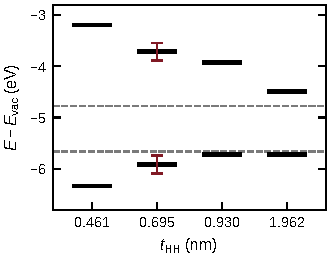
\includegraphics[width=\linewidth]{06_edges}
      \src{Upper bars $-$EA, lower bars $-$IP; dashed: bulk edges via the 2\,nm alignment. This work \sixlab{computed}.
        Maroon: $\pm0.17$\,eV vacuum-reference sensitivity of the polar film \sixlab{assumed}, not an error bound.}
    \end{column}
  \end{columns}
  \takeaway{Primary $\dEc$ law: 1 and 2\,nm films only; the polar film stays in the other laws.}
\end{frame}

% ---------------------------------------------------------------------------------------------------------------------
\begin{frame}{The gap opens by 0.34\,eV at 2\,nm and 0.90\,eV at 1\,nm}
  \sixdense
  \begin{columns}[T,onlytextwidth]
    \begin{column}{0.42\textwidth}
      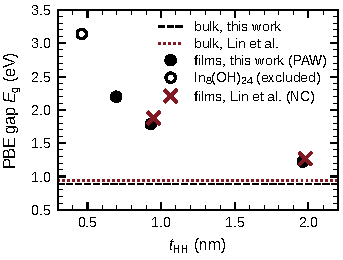
\includegraphics[width=\linewidth]{06_gaps}
      \src{PBE gaps. This work: PAW, 71\,Ry \sixlab{computed}. Crosses, dotted: Lin et al., norm-conserving, 140\,Ry,
        at their labels 0.95 and 1.98\,nm\sref[pp.~21540, 21542]{Lin2022}\xdef\sixlinfn{\the\value{footnote}}.}
    \end{column}
    \begin{column}{0.54\textwidth}
      \begin{itemize}
        \item Opening relative to the bulk PBE gap \lab{computed}:
          \begin{align*}
            \dEg(1.962\,\mathrm{nm}) &= 1.2239 - 0.8887 = 0.335\,\mathrm{eV}\\
            \dEg(0.930\,\mathrm{nm}) &= 1.7885 - 0.8887 = 0.900\,\mathrm{eV}
          \end{align*}
        \item Lin et al.\footnotemark[\sixlinfn], same recipe: $+0.33$\,eV at 1.98\,nm, $+0.94$\,eV at 0.95\,nm.
          Differences 0.005 and 0.04\,eV, inside the pre-registered 0.1\,eV \lab{derived}.
        \item Bulk and 1\,nm gaps and masses lie 4--7\,\% below theirs\footnotemark[\sixlinfn], all with one sign. This
          points to the numerical setup (PAW 71\,Ry against norm-conserving 140\,Ry) rather than to the films
          \lab{inferred}.
        \item Relaxation is essential: as built, the 1\,nm film opened the gap by only 0.07\,eV \lab{computed}.
      \end{itemize}
    \end{column}
  \end{columns}
  \takeaway{The 1 and 2\,nm openings reproduce an independent PBE study within 0.04\,eV.}
\end{frame}

% ---------------------------------------------------------------------------------------------------------------------
\begin{frame}{The gap law is well determined; the $\dEc$ law is not}
  \sixdense
  \begin{columns}[T,onlytextwidth]
    \begin{column}{0.38\textwidth}
      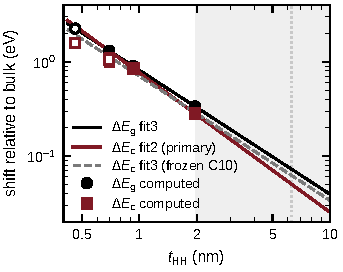
\includegraphics[width=\linewidth]{06_laws}
      \src{Open: 0.461\,nm (excluded); 0.695\,nm $\dEc$, bar: $\pm0.17$\,eV vacuum-reference sensitivity
        \sixlab{assumed}. Lines: $y = a\,t^{-p}$ \sixlab{fitted}; dotted: 6.3\,nm; grey: beyond the thickest film
        (extrapolation).}
    \end{column}
    \begin{column}{0.58\textwidth}
      \begingroup\scriptsize
      \renewcommand{\arraystretch}{1.05}
      \begin{tabular}{@{}l c c c@{}}
        \toprule
        law (points; $t = \tHH$ in nm) & $a$ (eV) & $p$ & 6.3\,nm (eV) \\
        \midrule
        $\dEg$ fit3 (0.695, 0.930, 1.962) & 0.815 & 1.316 & 0.072 \\
        $\dEc$ fit2, primary (0.930, 1.962) & 0.762 & 1.478 & 0.050 \\
        $\dEc$ fit3, frozen C10 (three points) & 0.702 & 1.318 & 0.062 \\
        \bottomrule
      \end{tabular}\par\endgroup
      \begin{itemize}
        \item $\dEg$: three points within 0.5\,\% of the law; leave-one-out $p = 1.29$--1.32 \lab{fitted};
          $\sigma_p = 0.007$ is scatter only (1 dof).
        \item $\dEc$: two clean points, no residual freedom. With the polar point $p = 1.32$ (leave-one-out
          0.76--1.48); moving it by $\mp0.17$\,eV gives 0.075 or 0.053\,eV at 6.3\,nm \lab{fitted}.
        \item A constant $\dEv \approx -0.053$\,eV lowers the $\dEg$ exponent (1.32 against 1.48): the laws are not
          interchangeable \lab{derived}.
        \item Every law is crystalline (001), PBE, one termination, used 3$\times$ beyond its data at 6.3\,nm; $\sigma$
          omits these errors and the untested field effect on the 0.695\,nm gap.
      \end{itemize}
    \end{column}
  \end{columns}
  \takeaway{$\dEc$ at 6.3\,nm is known only as a range, 0.050--0.075\,eV, set by the choice of fit.}
\end{frame}

% ---------------------------------------------------------------------------------------------------------------------
\begin{frame}{The conduction band takes 84 to 94\,\% of the gap opening}
  \sixdense
  \begin{columns}[T,onlytextwidth]
    \begin{column}{0.40\textwidth}
      {\centering
      \begin{tikzpicture}[x=1mm,y=1mm,font=\scriptsize]
        % energies relative to the bulk valence-band maximum, 15 mm per eV
        \draw[rulegrey,dashed,line width=0.5pt] (-1,0) -- (47,0);
        \draw[rulegrey,dashed,line width=0.5pt] (-1,13.33) -- (47,13.33);
        \node[anchor=east,inkgrey] at (-1,0) {$E_{\mathrm{v}}^{\mathrm{bulk}}$};
        \node[anchor=east,inkgrey] at (-1,13.33) {$E_{\mathrm{c}}^{\mathrm{bulk}}$};
        % bulk
        \draw[line width=1.3pt] (0,0) -- (12,0);
        \draw[line width=1.3pt] (0,13.33) -- (12,13.33);
        \draw[{Stealth[length=1.3mm]}-{Stealth[length=1.3mm]},line width=0.5pt] (4,0.4) -- (4,12.93);
        \node[anchor=west] at (4.5,6.7) {0.889};
        % 1.962 nm
        \draw[line width=1.3pt] (17,-0.81) -- (29,-0.81);
        \draw[line width=1.3pt] (17,17.55) -- (29,17.55);
        \draw[{Stealth[length=1.3mm]}-{Stealth[length=1.3mm]},line width=0.5pt] (20.5,-0.41) -- (20.5,17.15);
        \node[anchor=west] at (21.0,8.4) {1.224};
        \draw[-{Stealth[length=1.3mm]},ntumaroon,line width=0.8pt] (27.5,13.33) -- (27.5,17.35);
        \node[anchor=south] at (23,17.9) {$+0.281$};
        \node[anchor=north] at (23,-1.2) {$-0.054$};
        % 0.930 nm
        \draw[line width=1.3pt] (34,-0.78) -- (46,-0.78);
        \draw[line width=1.3pt] (34,26.05) -- (46,26.05);
        \draw[{Stealth[length=1.3mm]}-{Stealth[length=1.3mm]},line width=0.5pt] (37.5,-0.38) -- (37.5,25.65);
        \node[anchor=west] at (38.0,8.4) {1.789};
        \draw[-{Stealth[length=1.3mm]},ntumaroon,line width=0.8pt] (44.5,13.33) -- (44.5,25.85);
        \node[anchor=south] at (40,26.4) {$+0.848$};
        \node[anchor=north] at (40,-1.2) {$-0.052$};
        % column labels
        \node[anchor=north] at (6,-5.0) {bulk};
        \node[anchor=north] at (23,-5.0) {1.962\,nm};
        \node[anchor=north] at (40,-5.0) {0.930\,nm};
      \end{tikzpicture}\par}
      \src{To scale, eV. Black arrows: gaps; maroon: $\dEc$ (value above); $\dEv$ below each film. 2\,nm: two-step
        alignment; 1\,nm: 2\,nm value plus EA/IP differences. This work \sixlab{computed}.}
    \end{column}
    \begin{column}{0.56\textwidth}
      \begingroup\scriptsize
      \renewcommand{\arraystretch}{1.12}
      \setlength{\tabcolsep}{4.5pt}
      \begin{tabular}{@{}l c c c c@{}}
        \toprule
        film, alignment route & $\dEc$ & $\dEv$ & $\dEv$, EMA & CB share \\
        \midrule
        1.962\,nm, two-step & $+0.281$ & $-0.054$ & $-0.016$ & 0.84 / 0.95 \\
        \quad double average & $+0.287$ & $-0.049$ & & 0.86 \\
        0.930\,nm, 2\,nm + EA/IP & $+0.848$ & $-0.052$ & $-0.061$ & 0.94 / 0.93 \\
        \quad two-step$^{a}$ & $+0.819$ & $-0.081$ & & 0.91 \\
        \bottomrule
      \end{tabular}\par\endgroup
      \src{Energies in eV; CB share: DFT / EMA. $^{a}$No bulk-like interior; not used. EMA: Kane-consistent, hole
        energy $\varepsilon_1m_b/m_h$ with $\varepsilon_1 = \dEc(1+\alpha\dEc)$, $m_h = 3.2\,m_0$ (lightest)
        \sixlab{derived}.}
      \begin{itemize}
        \item Same termination: $\dEc(1) - \dEc(2) = \mathrm{EA}(2) - \mathrm{EA}(1) = +0.567$\,eV,
          $\dEv(1) - \dEv(2) = \mathrm{IP}(2) - \mathrm{IP}(1) = +0.002$\,eV \lab{computed}.
        \item EMA agrees at 1\,nm. At 2\,nm the computed $|\dEv|$ is about 38\,meV larger, beyond the route spread
          (5\,meV) and plateau flatness (8\,meV): unexplained \lab{unresolved}.
        \item The device model uses only $\dEc$ and the gap: $\dEv \approx -0.05$\,eV does not move the electron barrier.
      \end{itemize}
    \end{column}
  \end{columns}
  \takeaway{At 2\,nm the conduction band rises by 0.28\,eV; the V1 device model assumed 0.35\,eV.}
\end{frame}

% ---------------------------------------------------------------------------------------------------------------------
\begin{frame}{Envelope models bracket the shift but do not predict it}
  \sixdense
  \begin{columns}[T,onlytextwidth]
    \begin{column}{0.41\textwidth}
      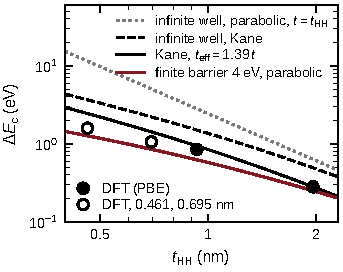
\includegraphics[width=0.96\linewidth]{06_models}
      \src{Bulk PBE $m_b = 0.1541\,m_0$, $\alpha = 0.58$\,eV$^{-1}$; dotted, dashed, maroon \sixlab{derived}. Solid:
        box $1.39\,\tHH$, fitted to the 1.962\,nm point \sixlab{fitted}.}
    \end{column}
    \begin{column}{0.55\textwidth}
      \begin{itemize}
        \item Infinite well, $t = \tHH$:
          $E_n - \Ec = \dfrac{\hbar^2\pi^2n^2}{2m_bt^2} = \dfrac{0.376\,\mathrm{eV\,nm^2}}{(m_b/m_0)\,t^2}\,n^2$\\
          0.634\,eV at 1.962\,nm, $2.3\times$ the computed value \lab{derived}.
        \item Kane band\sref{Kane1957}, $E(1+\alpha E) = \hbar^2k^2/2m_b$: the fitting box grows from $1.39\,\tHH$
          (1.962\,nm) to $1.49\,\tHH$ (0.930\,nm); fixed at 2\,nm it gives 0.94\,eV at 1\,nm, not 0.848
          \lab{derived}.
        \item 4\,eV barrier, $m_0$ outside, $F'/m$ continuous\sref{Bastard1981}: 0.25\,eV at 1.962\,nm, 0.63\,eV at
          0.930\,nm. The envelope leaks 0.6\,nm per side: the result rests on a boundary condition that is undetermined
          at an atomic surface \lab{derived}.
        \item The bixbyite cell is 1.03\,nm: the 1\,nm film is thinner than one cell, the 2\,nm film spans two. For
          every film here envelope theory is a parametrisation to be tested.
      \end{itemize}
    \end{column}
  \end{columns}
  \takeaway{Not refuted, but not predictive: the device model takes $\dEc$ from DFT, not from a box.}
\end{frame}

% ---------------------------------------------------------------------------------------------------------------------
\begin{frame}{HSE06 changes the 1\,nm gap opening by only 6 to 11\,\%}
  \sixdense
  \begin{columns}[T,onlytextwidth]
    \begin{column}{0.41\textwidth}
      \begingroup\scriptsize
      \renewcommand{\arraystretch}{1.12}
      \setlength{\tabcolsep}{3.5pt}
      \begin{tabular}{@{}l c c c@{}}
        \toprule
        Kohn--Sham gaps (eV) & bulk & 1\,nm film & $\dEg$ \\
        \midrule
        PBE & 0.9204 & 1.8068 & 0.8864 \\
        HSE06, $q = 1$ & 2.1080 & 3.0475 & 0.9395 \\
        \midrule
        ratio $r$ & & & 1.060 \\
        \bottomrule
      \end{tabular}\par\endgroup
      \src{SG15 norm-conserving\srefs{Hamann2013,Schlipf2015}, 80\,Ry, both functionals at the PBE geometries. Bulk PBE:
        VBM off $\Gamma$ (direct gap at $\Gamma$ 0.9216\,eV). This work \sixlab{computed}.}
      \vspace{2mm}
      \begingroup\scriptsize
      \renewcommand{\arraystretch}{1.12}
      \begin{tabular}{@{}c c@{}}
        \toprule
        HSE06 bulk mass $m_b$ ($m_0$) & Kane-model $r$ \\
        \midrule
        0.159 & 1.158 \\
        0.170 & 1.095 \\
        0.193 & 0.983 \\
        \bottomrule
      \end{tabular}\par\endgroup
      \src{Masses estimated from the HSE06 SCF grid; $r$ from a Kane band with $\alpha = 0.58\times0.920/2.108
        = 0.253$\,eV$^{-1}$ \sixlab{derived}.}
    \end{column}
    \begin{column}{0.56\textwidth}
      \begin{itemize}
        \item HSE06\srefs{Heyd2003,Heyd2006,Krukau2006} at fixed geometry, norm-conserving (PAW exact exchange had not
          finished its first step after 4.5\,h on an H100); only $r$ is transferred.
        \item $r = 1.060$ meets the pre-registered 10\,\% criterion; a $3\times3\times3$ exchange $q$ grid lowers the bulk
          HSE06 gap by 42\,meV, so $r = 1.06$--1.11 \lab{computed}.
        \item PAW and norm-conserving PBE openings agree within 1.6\,\% \lab{computed}: HSE-corrected 1\,nm opening
          0.95--1.00\,eV, gap 3.06\,eV \lab{derived}; 2\,nm gap 2.44--2.46\,eV if $r$ transfers (amendment A23)
          \lab{assumed}.
        \item Why $r\approx1$: HSE06 makes the band heavier but less non-parabolic; a Kane band with
          $\alpha\propto1/\Eg$ (assumed) gives 0.98--1.16, bracketing $r$ without deriving it \lab{derived}.
      \end{itemize}
    \end{column}
  \end{columns}
  \takeaway{PBE misses the gap but not the 1\,nm shift; other thicknesses assume the same $r$.}
\end{frame}

% ---------------------------------------------------------------------------------------------------------------------
\begin{frame}{One subband at 2\,nm, but not reliably at 6.3\,nm}
  \sixdense
  \begin{columns}[T,onlytextwidth]
    \begin{column}{0.42\textwidth}
      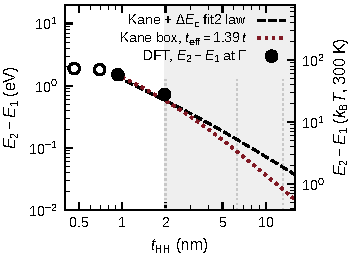
\includegraphics[width=\linewidth]{06_subbands}
      \src{Spacing $E_2-E_1$ of the lowest two conduction levels at $\Gamma$: DFT (open: 0.461, 0.695\,nm)
        \sixlab{computed}; Kane estimates \sixlab{derived}. Dotted: device thicknesses 2.0, 6.3 and 13.2\,nm; grey:
        beyond the thickest film (extrapolation).}
    \end{column}
    \begin{column}{0.54\textwidth}
      \begin{itemize}
        \item Crystalline films, PBE: $E_2 - E_1 = 0.72$\,eV at 1.962\,nm and 1.50\,eV at 0.930\,nm;
          $(E_2-E_1)/E_1 = 2.56$ and 1.77, below the parabolic 3 \lab{computed}.
        \item One occupied subband needs $E_2 - E_1 \gg \kT$. Kane band with the $\dEc$ law: 0.59\,eV ($23\,\kT$) at
          1.962\,nm, 0.14\,eV ($5\,\kT$) at 6.3\,nm, 0.05\,eV ($2\,\kT$) at 13.2\,nm \lab{derived}.
        \item The 6.3 and 13.2\,nm values extrapolate the law 3 to 7 times; a box of width $1.39\,t$ gives
          0.088\,eV ($3.4\,\kT$) at 6.3\,nm \lab{derived}. Degenerate filling is ignored.
        \item The device films are amorphous or nanocrystalline: whether this transfers is registered test H-K
          (Part 11).
      \end{itemize}
    \end{column}
  \end{columns}
  \takeaway{Estimate for a crystalline PBE film: one subband at 2\,nm, one or two at 6.3\,nm, several at 13\,nm
    \lab{derived}.}
\end{frame}

% 07_masses.tex -- Part 7, electron and hole masses. Sources: research_monograph/chapters/M09_masses_parameters.tex
% (sec:mono-mass-bulk, sec:mono-mass-electrons, sec:mono-mass-holes, tab:mono-mass-laws, tab:mono-mass-tcad),
% M05_confinement_theory.tex (sec:mono-conf-kane, sec:mono-conf-subband, sec:mono-conf-test, tab:mono-conf-test),
% M03_literature_materials.tex (sec:mono-lit-mass), evidence/FACT_REGISTRY.tsv (FACT-004, 005, 006, 026a-d, 027, 047,
% 060, 061, 062), evidence/CLAIM_SOURCE_MAP.tsv (C039, C040, M004), evidence/derived/confinement_analysis.json,
% appendices/MG_corrections.tex (X6, V5, V10), qe_workflow/cern_htcondor/results/RESULTS_LOG.md (2026-10-14 entry),
% qe_workflow/analysis_2026-10-13_full/bands_masses/BANDS_MASSES.md (section 2.3 checks), chapters/13_dft_rev.tex
% (experimental lattice 10.117 A).
% Figures: tools/fig_07_masses.py (data: qe_workflow/analysis_2026-10-13_full/bands_masses/out/b01_masses.json,
% b03_gaps_laws.json, b05_holes.json; evidence/derived/confinement_analysis.json).
% Note: frame bodies start with a command, never with a brace group (beamer would read a subtitle).
% denser slides: footnotesize bullets, local to the frame in which it is called
\providecommand{\sevdense}{\setbeamerfont{itemize/enumerate body}{size=\footnotesize}%
  \setbeamerfont{itemize/enumerate subbody}{size=\footnotesize}}
% evidence label inside a \src line: same vocabulary as \lab, but at the (tiny) size of the source line
\providecommand{\sevsrclab}[1]{[\textsc{\MakeLowercase{#1}}]}
\providecommand{\sevNv}{N_{\mathrm{v}}}
% pull the frame body up towards the title rule (as in Parts 5 and 8); keeps clear space above the take-away
\providecommand{\sevTop}{\vspace{-3mm}}

\partslide{Part 7}{Electron and hole masses}

% ---------------------------------------------------------------------------------------------------------------------
\begin{frame}{Bulk electrons: a Kane band, 26\,\% lighter than measured}
  \sevdense\sevTop
  \begin{columns}[T,onlytextwidth]
    \begin{column}{0.47\textwidth}
      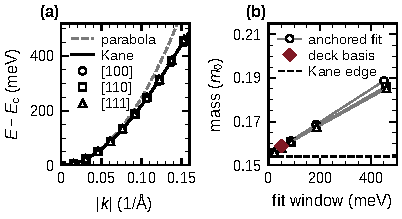
\includegraphics[width=\linewidth]{07_bulk_cb}
      \src{(a) Bulk conduction band near $\Gamma$; solid: Kane band; dashed: parabola, same $m_b$. (b) Mass by fit
        basis: parabolas anchored at $\Gamma$ over 25--450\,meV windows, four-point deck basis, Kane band edge. This work,
        PAW-PBE \sevsrclab{computed}.}
    \end{column}
    \begin{column}{0.49\textwidth}
      \begin{itemize}
        \item $E(1+\alpha E) = \hbar^2k^2/2m_b$ fits [100], [110], [111] to 0.45\,eV: $m_b$ = 0.1541\,$m_0$ (isotropic
          within 0.2\,\%), $\alpha$ = 0.58\,eV$^{-1}$ (0.55--0.63). Other bases: four-point (deck) 0.1588\,$m_0$,
          anchored parabolas 0.156--0.189\,$m_0$ \lab{computed}.
        \item Measured: 0.208\,$\pm$\,0.006\,$m_0$\sref[p.~225102-1]{Stokey2021}; 0.18\,$m_0$ at zero density, about 0.4\,$m_0$ at
          $10^{21}$\cmcu\sref{Feneberg2016} \lab{measured}; PBE Kane optical mass $m_b(1+2\alpha\EF)$ there
          0.39\,$m_0$ ($\EF$ beyond the fit window) \lab{derived}.
        \item Caveats: a polaron (Fr\"ohlich coupling near one: +15\,\%) could explain half of the 26\,\%
          \lab{hypothesis}; the two-band gap is not the fundamental one (dipole-forbidden edge\sref{Walsh2008}).
      \end{itemize}
    \end{column}
  \end{columns}
  \takeaway{Decks: measured 0.208\,$m_0$ plus the PBE increase on the deck basis, 0.1114\,$t^{-1.2611}$\,$m_0$.}
\end{frame}

% ---------------------------------------------------------------------------------------------------------------------
\begin{frame}{Confinement raises the mass; extrapolated, little beyond 2\,nm}
  \sevdense\sevTop
  \begin{columns}[T,onlytextwidth]
    \begin{column}{0.43\textwidth}
      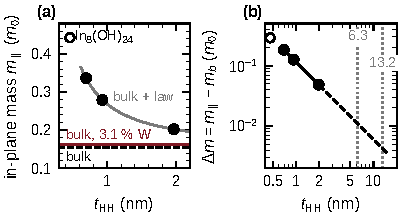
\includegraphics[width=\linewidth]{07_film_masses}
      \src{(a) In-plane band-edge mass of the relaxed films. (b) Increase over bulk with the fitted law; dashed:
        extrapolated. Open: In$_8$(OH)$_{24}$, outside every law. This work, PAW-PBE \sevsrclab{computed},
        law \sevsrclab{fitted}.}
    \end{column}
    \begin{column}{0.53\textwidth}
      \begin{itemize}
        \item In-plane band-edge masses (2-D DOS, Kane basis): 0.443, 0.337, 0.279, 0.203\,$m_0$ from 0.461 to
          1.962\,nm; in-plane $\alpha$ 0.24--0.47\,eV$^{-1}$ \lab{computed}.
        \item Fit, 0.695--1.962\,nm, one residual degree of freedom, band-edge basis: $\Delta m$ =
          0.1145\,$t^{-1.2755}$\,$m_0$ ($t = \tHH$ in nm); 0.047\,$m_0$ at 2.0\,nm \lab{fitted}.
        \item The device decks use the deck-basis law 0.1114\,$t^{-1.2611}$\,$m_0$ (previous slide); both laws
          give 0.011 and 0.004\,$m_0$ at 6.3 and 13.2\,nm, extrapolated \lab{fitted}.
        \item Deck basis at 2\,nm: 0.206\,$m_0$. Checks: GPU against CPU 0.0006\,$m_0$, 15--35\,\AA{} vacuum
          0.0002\,$m_0$; relaxation: +18\,\% at 1\,nm \lab{computed}.
        \item 3.1\,\% W in bulk: same shape, 5\,\% heavier, 0.161--0.163\,$m_0$ \lab{computed}; no W-film band run.
      \end{itemize}
    \end{column}
  \end{columns}
  \takeaway{Beyond 2\,nm confinement adds little to the electron mass: 0.011\,$m_0$ at 6.3\,nm \lab{fitted}.}
\end{frame}

% ---------------------------------------------------------------------------------------------------------------------
\begin{frame}{No-fit Kane test: 1\,\% off at 2\,nm, 10\,\% off at 1\,nm}
  \sevdense\sevTop
  \begingroup\small\setlength{\abovedisplayskip}{2pt}\setlength{\belowdisplayskip}{2pt}%
  Kane band\sref{Kane1957} confined with $k_z = n\pi/t$, expanded at $k_\parallel = 0$:
  \begin{equation*}
    E(1+\alpha E) = \varepsilon_n + \frac{\hbar^2k_\parallel^2}{2m_b},\quad
    \varepsilon_n = \frac{\hbar^2\pi^2n^2}{2m_bt^2}
    \quad\Longrightarrow\quad
    m_\parallel = m_b\,(1+2\alpha E_1),\quad \alpha_\parallel = \frac{\alpha}{1+2\alpha E_1}
  \end{equation*}
  where $E_1$ = computed $\dEc$; bulk fit (to 0.45\,eV) $m_b$ = 0.1541\,$m_0$, $\alpha$ = 0.58\,eV$^{-1}$: nothing
  is adjusted.\par\endgroup
  \vspace{1mm}
  \begin{columns}[T,onlytextwidth]
    \begin{column}{0.47\textwidth}
      \begingroup\scriptsize
      \setlength{\tabcolsep}{3.2pt}
      \renewcommand{\arraystretch}{1.1}
      \begin{tabular*}{\linewidth}{@{\extracolsep{\fill}}l c c c r@{}}
        \toprule
        $\tHH$ (nm) & $\dEc$ (eV) & $m_\parallel$ comp. & $m_\parallel$ Kane & Kane/comp.\,\textminus\,1 \\
        \midrule
        1.962 & 0.281 & 0.203 & 0.204 & +0.7\,\% \\
        0.930 & 0.848 & 0.279 & 0.306 & +9.6\,\% \\
        0.695$^a$ & 1.059 & 0.337 & 0.343 & +1.9\,\% \\
        0.461$^b$ & 1.585 & 0.443 & 0.437 & \textminus1.3\,\% \\
        \bottomrule
      \end{tabular*}\par\endgroup
      \src{Masses in $m_0$; comp.: computed in-plane 2-D DOS band-edge mass. $^a$Polar film, $\dEc$ \textpm\,0.17\,eV.
        $^b$In$_8$(OH)$_{24}$. FACT-027 \sevsrclab{derived}.}
    \end{column}
    \begin{column}{0.49\textwidth}
      \begin{itemize}
        \item Tests: 1.962 and 0.930\,nm. The 0.930\,nm test uses the band at 0.85\,eV, beyond the fit window; the
          two-step $\dEc$ (0.819\,eV) still gives 0.300\,$m_0$ \lab{derived}.
        \item The 0.695 and 0.461\,nm films agree within 2\,\% but do not test it: 1.585\,eV is far beyond the fit
          window, and \textpm0.17\,eV moves the 0.695\,nm prediction by \textpm9\,\%.
      \end{itemize}
    \end{column}
  \end{columns}
  \takeaway{At 2\,nm the mass increase is consistent, within 1\,\%, with the bulk non-parabolicity at the subband
    energy \lab{derived}.}
\end{frame}

% ---------------------------------------------------------------------------------------------------------------------
\begin{frame}{The mass law and the $\dEc$ law are one input, not two}
  \sevdense\sevTop
  \begin{columns}[T,onlytextwidth]
    \begin{column}{0.47\textwidth}
      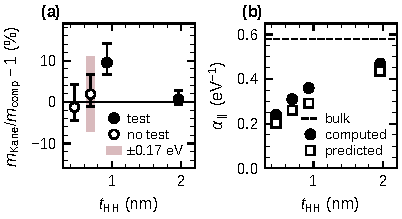
\includegraphics[width=\linewidth]{07_kanetest}
      \src{(a) Kane prediction against the computed in-plane mass; bars: $\alpha$ = 0.55--0.63; shaded: \textpm0.17\,eV
        in the polar 0.695\,nm film; open: no test. (b) In-plane non-parabolicity, computed and $\alpha/(1+2\alpha
        E_1)$. This work \sevsrclab{derived}. Claim M004; review correction V5.}
    \end{column}
    \begin{column}{0.49\textwidth}
      \begin{itemize}
        \item The bulk $\alpha$ range (bars) moves the 0.930\,nm prediction only to 0.298--0.319\,$m_0$, against
          0.279\,$m_0$ computed \lab{derived}.
        \item $\alpha/(1+2\alpha E_1)$ lies 7--19\,\% below the computed $\alpha_\parallel$, with the right trend
          \lab{derived}.
        \item The total in-plane mass follows from $\dEc$ within 10\,\%, $\Delta m$ itself within about 20\,\%; the
          fitted exponents, 1.28 ($\Delta m$) and 1.48 ($\dEc$), diverge when extrapolated \lab{derived}.
        \item A device model that uses both laws therefore carries one independent first-principles input, not two
          (Part~10).
      \end{itemize}
    \end{column}
  \end{columns}
  \takeaway{The two laws are one input; at 6.3 and 13.2\,nm both are extrapolated \lab{derived}.}
\end{frame}

% ---------------------------------------------------------------------------------------------------------------------
\begin{frame}{No single hole mass; \textit{N}\textsubscript{v} is about 200 times the deck value}
  \sevdense\sevTop
  \begin{columns}[T,onlytextwidth]
    \begin{column}{0.47\textwidth}
      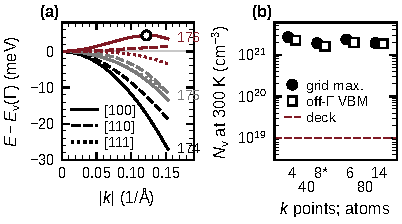
\includegraphics[width=\linewidth]{07_holes}
      \src{(a) Valence bands near $\Gamma$; circle: global maximum. (b) $\sevNv$ from the Boltzmann-integrated valence
        DOS, two energy references; $k$-mesh convergence not established. Grids: 40-atom primitive cell, 4 and 8 $k$
        points ($^*$at the experimental lattice, 10.117\,\AA); 80-atom cell, 6 and 14 $k$ points. Dashed: deck value.
        This work, PAW-PBE \sevsrclab{computed}.}
    \end{column}
    \begin{column}{0.49\textwidth}
      \begin{itemize}
        \item Three-fold degenerate top with a 4.4\,meV camel back (${\ll}\,\kT$). Curvature masses
          3.2--7.9\,$m_0$ (band 174), 6.9--19.8\,$m_0$ (175); band 176 rises along [100] and [110] \lab{computed}.
        \item Valence DOS: $\sevNv$ = 1.6--2.7\,$\times$\,$10^{21}$\cmcu{} (300\,K), $m_{h,\mathrm{DOS}}$ =
          16--22\,$m_0$; $k$-mesh convergence not established \lab{computed}.
        \item Decks: $\sevNv = 10^{19}$\cmcu{} (0.54\,$m_0$), electrons only \lab{assumed}.
        \item Computed $\sevNv$: $n_i$ (2\,nm) rises from 5.0\,$\times$\,$10^{-10}$ to 6.7\,$\times$\,$10^{-9}$\cmcu;
          equilibrium SRH generation ${\le}$\,3.4\,$\times$\,$10^{-3}$\,cm$^{-3}$\,s$^{-1}$, negligible \lab{derived}.
        \item Holes are predicted to self-trap\sref{Varley2012}; $\sevNv$ is a free-hole band integral.
      \end{itemize}
    \end{column}
  \end{columns}
  \takeaway{Only $\sevNv$ is usable for holes; in the electron-only decks its effect is negligible \lab{derived}.}
\end{frame}

% 08_tungsten.tex -- Part 8, tungsten as a donor in crystalline In2O3. Sources: research_monograph/chapters/
% M10_w_and_vacancies.tex (sec:mono-w-cells, sec:mono-w-site, sec:mono-w-level, tab:mono-w-cells, tab:mono-w-open,
% keyresult), M06_defect_theory.tex (sec:mono-defect-hydrogenic, sec:mono-defect-resonant), M03_literature_materials.tex
% (sec:mono-lit-w), M08_c10_campaign.tex (tab:mono-c10-models: donors 2.5e17 V1 fitted, accumulation 5.6e19),
% 13_dft_rev.tex l.1231 (Shannon radius sums incl. W5+), appendices/MG_corrections.tex (X1, X7, X9, X11);
% evidence/FACT_REGISTRY.tsv (FACT-004, 005, 040-048, 080, 082); evidence/derived/defect_estimates.json;
% research_record/03_CLAIMS_LEDGER.yaml (C022); qe_workflow/cern_htcondor/results/RESULTS_LOG.md (2026-09-29,
% 2026-09-30, 2026-10-05 CORRECTION, 2026-10-14 C022 caveat); qe_workflow/analysis_2026-10-13_full/out/
% f09_iwo_bulk.json, f10_iwo_slabs.json. Figures: tools/fig_08_tungsten.py (data: f09/f10 JSON, raw bands.out of
% iwo_W8b and iwo_W24d, bands_masses/out/b01_masses.json). Crystalline cells only; no amorphous quantity appears.
% Note: frame bodies start with a command, never with a brace group (beamer would read a subtitle).
\partslide{Part 8}{Tungsten as a donor}

% denser slides: footnotesize bullets, local to the frame in which it is called
\providecommand{\eightdense}{\setbeamerfont{itemize/enumerate body}{size=\footnotesize}%
  \setbeamerfont{itemize/enumerate subbody}{size=\footnotesize}}
% pull the frame body up towards the title rule (as \fiveTop in Part 5)
\providecommand{\eightTop}{\vspace{-4mm}}

% ---------------------------------------------------------------------------------------------------------------------
\begin{frame}{W cells donate 1.4--3.0$\times10^{21}$\cmcu, far above the Mott density}
  \eightdense\eightTop
  \begingroup\scriptsize
  \renewcommand{\arraystretch}{1.02}
  \begin{tabularx}{\textwidth}{@{}X l c l c@{}}
    \toprule
    cell & composition & W / cations & W site & donated density \\
    \midrule
    bulk, 80 atoms, PBE lattice $a = 10.3061$\,\AA & In$_{31}$WO$_{48}$ & 3.1\,\% & 24d or 8b & $2.7\times10^{21}$\cmcu \\
    relaxed 1\,nm film & In$_{23}$WO$_{48}$H$_{24}$ & 4.2\,\% & central 24d & $3.0\times10^{21}$\cmcu \\
    relaxed 2\,nm film & In$_{55}$WO$_{96}$H$_{24}$ & 1.8\,\% & central 24d & $1.4\times10^{21}$\cmcu \\
    \bottomrule
  \end{tabularx}\par\endgroup
  \src{PAW-PBE, 71/568\,Ry; Marzari--Vanderbilt (MV) smearing 0.01\,Ry; ions relaxed at fixed cell (bulk on
    3$\times$3$\times$3, final SCF on 4$\times$4$\times$4); claim C022; this work \lab{computed}.}
  \begin{columns}[T,onlytextwidth]
    \begin{column}{0.53\textwidth}
      \begin{itemize}
        \item The device paper credits W with ``smoother charge delocalization''\sref[p.~4]{Januar2026}. Here: where
          the W level lies and where its electrons go.
        \item Hydrogenic donor: $E_D \approx 25$\,meV, Mott density $n_c \approx 9\times10^{17}$\cmcu{} \lab{derived}
          (Part~12; derivation in backup).
        \item Device model (Part~4, open circles): donors below $n_c$ \lab{fitted}; on-state channel (2\,nm film, 2\,V
          overdrive) degenerate \lab{derived}.
      \end{itemize}
    \end{column}
    \begin{column}{0.44\textwidth}
      \centering
      \begin{tikzpicture}[x=1mm,y=1mm,font=\scriptsize,line width=0.5pt]
        % log axis 1e17 .. 1e22, 11 mm per decade
        \draw (0,0) -- (55,0);
        \foreach \e/\x in {17/0,18/11,19/22,20/33,21/44,22/55} {
          \draw (\x,0) -- (\x,1.2);
          \node[anchor=north,inner sep=1.2pt] at (\x,0) {$10^{\e}$};
        }
        \node[anchor=north] at (27.5,-4.0) {electron density (cm$^{-3}$)};
        % Mott density 9.1e17: log10 = 17.96 -> 10.54 mm
        \draw (10.54,0) -- (10.54,10.5);
        \node[anchor=south,align=center] at (10.54,10.5) {Mott density $n_c$\\[-0.3mm]$9\times10^{17}$};
        % W cells 1.4e21 .. 3.0e21: log10 = 21.146 .. 21.477 -> 45.6 .. 49.2 mm
        \draw[line width=2.4pt] (45.6,3.2) -- (49.2,3.2);
        \draw (45.6,0) -- (45.6,3.2);
        \draw (49.2,0) -- (49.2,3.2);
        \draw[rulegrey] (47.4,4.4) -- (47.4,10.5);
        \node[anchor=south,align=center] at (47.4,10.5) {W cells\\[-0.3mm]1.4--3.0$\times10^{21}$};
        \draw[{Stealth[length=1.6mm]}-{Stealth[length=1.6mm]},ntumaroon,line width=0.7pt] (11.3,6.6) -- (44.8,6.6);
        \node[anchor=south,ntumaroon] at (28,6.9) {1500--3300 times};
        % device model (M08): donors 2.5e17 -> 17.398 -> 4.38 mm; on-state 5.6e19 -> 19.748 -> 30.23 mm
        \draw[fill=white] (4.38,0) circle (0.75mm);
        \node[anchor=south,align=center,inner sep=1pt] at (4.0,1.0) {donors\\[-0.6mm]$2.5\times10^{17}$};
        \draw[fill=white] (30.23,0) circle (0.75mm);
        \node[anchor=south,inner sep=1pt] at (30.23,1.0) {on-state $5.6\times10^{19}$};
      \end{tikzpicture}
      \src{W cells: 3\,e per W (formal count) per cell volume (films: H--H thickness) \lab{derived}.
        Device model: donors \lab{fitted}; on-state \lab{derived}.}
    \end{column}
  \end{columns}
  \takeaway{The cells hold no bound hydrogenic state; they locate the W-5d level in the band.}
\end{frame}

% ---------------------------------------------------------------------------------------------------------------------
\begin{frame}{W prefers 24d by 0.258\,eV; W--O bonds consistent with W$^{6+}$}
  \eightdense\eightTop
  \begin{columns}[T,onlytextwidth]
    \begin{column}{0.42\textwidth}
      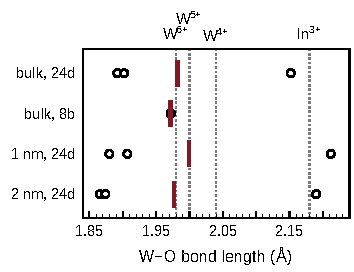
\includegraphics[width=\linewidth]{08_bonds}
      \src{W--O bonds of the relaxed cells (circles; each value occurs twice on 24d, six times on 8b); bars: mean
        bond; dotted: Shannon radius sums for six-fold cations with O$^{2-}$ (1.38\,\AA). This
        work, PAW-PBE \lab{computed}.}
    \end{column}
    \begin{column}{0.55\textwidth}
      \begin{itemize}
        \item $\Delta E = E(\mathrm{8b}) - E(\mathrm{24d}) = 0.2579$\,eV (3$\times$3$\times$3 relaxation),
          0.2577\,eV (4$\times$4$\times$4) \lab{computed}.
        \item Three 24d sites per 8b site: $N_{\mathrm{24d}}/N_{\mathrm{8b}} = 3\exp(\Delta E/\kT) \approx 440$ at
          600\,K; 8b is practically empty at any processing temperature \lab{derived}.
        \item Mean W--O bond: bulk 1.982 (24d), 1.972\,\AA{} (8b); films 2.000 (1\,nm), 1.977\,\AA{} (2\,nm)
          \lab{computed}. Shannon sums\sref{Shannon1976}: 1.98 (W$^{6+}$), 2.00 (W$^{5+}$), 2.04\,\AA{} (W$^{4+}$).
        \item Bulk and 2\,nm means are consistent with W$^{6+}$; the 1\,nm mean sits at the W$^{5+}$ sum. An ionic-radius argument,
          not a charge measurement (record correction X11).
      \end{itemize}
    \end{column}
  \end{columns}
  \takeaway{W sits on 24d; formally W$^{6+}$, it leaves three electrons per W above the valence band.}
\end{frame}

% ---------------------------------------------------------------------------------------------------------------------
\begin{frame}{At 3\,e per cell the W-5d-rich state lies 1.2--1.8\,eV above $\Ec$}
  \eightdense\eightTop
  \begin{columns}[T,onlytextwidth]
    \begin{column}{0.42\textwidth}
      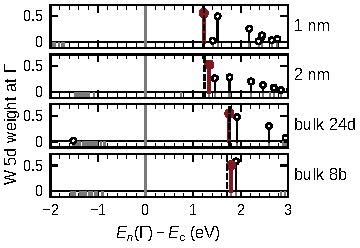
\includegraphics[width=\linewidth]{08_levels}
      \src{W-5d weight of each state at $\Gamma$ against its energy relative to the host conduction-band bottom $\Ec$; grey
        ticks: all states; dashed: $\EF$; maroon: $E_{\mathrm{W}}$, the first state above the host-band bottom with
        W 5d $\ge 0.3$ at $\Gamma$; in bulk 8b a state 0.10\,eV higher has 58\,\%. PBE, MV 0.01\,Ry. This work
        \lab{computed}.}
    \end{column}
    \begin{column}{0.55\textwidth}
      \begingroup\scriptsize
      \renewcommand{\arraystretch}{1.05}
      \begin{tabular*}{\linewidth}{@{\extracolsep{\fill}}l c c c@{}}
        \toprule
        cell (W site) & $\EF - \Ec$ & $E_{\mathrm{W}} - \Ec$ & $E_{\mathrm{W}} - \EF$ \\
        \midrule
        1\,nm film (24d) & 1.228 & 1.22 & $-0.005$ \\
        2\,nm film (24d) & 1.238 & 1.34 & $+0.103$ \\
        bulk (24d) & 1.763 & 1.76 & $+0.001$ \\
        bulk (8b) & 1.713 & 1.80 & $+0.090$ \\
        \bottomrule
      \end{tabular*}\par\endgroup
      \src{Energies in eV at $\Gamma$, at the computed filling (3\,e per cell, 1.4--3.0$\times10^{21}$\cmcu);
        $E_{\mathrm{W}}$: W-5d-rich level. Claim C022 \lab{computed}.}
      \begin{itemize}
        \item Resonant donor\sref{Swallow2020}: a level inside the band hybridises with it; the donor is ionised at
          any temperature, and the level fills only once $\EF$ reaches it \lab{theory}.
        \item In every cell a W-5d-rich state (50--60\,\% W 5d at $\Gamma$) lies 1.22--1.80\,eV above $\Ec$, within
          about 0.1\,eV of $\EF$ \lab{computed}.
        \item Not proof of pinning: a partly filled narrow level sits at $\EF$ by construction; 0.1\,eV is below the
          0.136\,eV smearing.
      \end{itemize}
    \end{column}
  \end{columns}
  \takeaway{At the cells' filling, $\EF$ has risen through the host band up to the W resonance.}
\end{frame}

% ---------------------------------------------------------------------------------------------------------------------
\begin{frame}{Most donated electrons fill the host band, not the W level}
  \eightdense\eightTop
  \begin{columns}[T,onlytextwidth]
    \begin{column}{0.40\textwidth}
      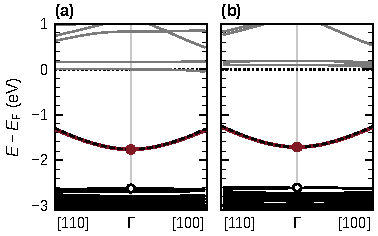
\includegraphics[width=\linewidth]{08_bands}
      \src{Bulk W cells, (a) 24d, (b) 8b. Black: valence bands (circle: top, band 351); maroon: host conduction band
        (352); grey: W-5d-rich and folded host bands; dashed: pure-bulk band shifted to the host minimum (nearly on
        the maroon curve: masses differ by 5\,\%); dotted: $\EF$. This work \lab{computed}.}
    \end{column}
    \begin{column}{0.57\textwidth}
      \begin{itemize}
        \item Of three electrons, the lowest host band holds 1.79 (24d), 1.93 (8b), 2.00 (1\,nm); the W-5d-rich band
          (half W 5d at $\Gamma$) 1.13, 0.95, 0.99 \lab{computed}.
        \item Kane band\sref{Kane1957} filled to the computed $\EF$:\vspace{-1.5mm}
          \[ N = \frac{\Omega\,k_F^3}{3\pi^2}, \quad \frac{\hbar^2k_F^2}{2m_b} = E(1+\alpha E), \quad E = \EF-\Ec \]
          \vspace{-3.8mm}\par
          $N$: electrons per cell, $k_F$: Fermi wave vector; $\Omega = 1094.6$\,\AA$^3$, $m_b = 0.162\,m_0$,
          $\alpha = 0.58$\,eV$^{-1}$ give 2.17 (24d), 2.04\,e (8b), above the computed 1.79, 1.93; a parabolic band
          gives 0.76, 0.73\,e \lab{derived}.
        \item W makes the bulk host band 5\,\% heavier (0.162 vs 0.1541\,$m_0$) and narrows the film gaps by 0.069
          (1\,nm), 0.148\,eV (2\,nm) \lab{computed}: consistent with band-gap renormalisation\sref{Hamberg1986}
          \lab{inferred}; strain not separated.
      \end{itemize}
    \end{column}
  \end{columns}
  \takeaway{A non-parabolic host band can hold two electrons per cell; a parabolic one cannot.}
\end{frame}

% ---------------------------------------------------------------------------------------------------------------------
\begin{frame}{Record correction X1: the ``deep W level'' was a band miscount}
  \eightdense\eightTop
  \begin{columns}[T,onlytextwidth]
    \begin{column}{0.52\textwidth}
      \centering
      \begin{tikzpicture}[x=0.89mm,y=10.5mm,font=\scriptsize,line width=0.5pt]
        % energy axis: E - E_F at Gamma (eV), 1 nm W film; levels: f10_iwo_slabs.json, bands 311-314
        \draw (0,-3.1) -- (0,0.4);
        \foreach \v in {-3,-2,-1,0} { \draw (0,\v) -- (1.2,\v); \node[anchor=east,inner sep=1.5pt] at (0,\v) {$\v$}; }
        \node[rotate=90,anchor=south,inner sep=1pt] at (-4.6,-1.35) {$E - \EF$ at $\Gamma$ (eV)};
        \draw[dashed] (2.5,0) -- (70,0);
        % column headers
        \node[anchor=south] at (15,0.5) {\textbf{30 Sep reading}};
        \node[anchor=south] at (50,0.5) {\textbf{corrected, 5 Oct}};
        % superseded reading
        \draw[rulegrey,line width=1pt] (3,-2.947) -- (13,-2.947);
        \node[anchor=west,inkgrey] at (14,-2.947) {311};
        \draw[line width=1pt] (3,-1.228) -- (13,-1.228);
        \node[anchor=west] at (14,-1.228) {``VB top'' (312)};
        \draw[ntumaroon,line width=1.4pt] (3,-0.005) -- (13,-0.005);
        \draw[line width=1pt] (3,0.185) -- (13,0.185);
        \node[anchor=west] at (14,0.30) {``CB bottom'' (314)};
        \node[anchor=north west,ntumaroon,align=left,inner sep=1pt] at (14,-0.06) {``W level'' (313),\\[-0.4mm]0.19\,eV below ``CB''};
        \node[anchor=west,inkgrey] at (3,-0.75) {``gap'' 1.22\,eV};
        % corrected reading
        \draw[line width=1pt] (41,-2.947) -- (51,-2.947);
        \node[anchor=west,align=left] at (52,-2.947) {VB top\\[-0.4mm]311: O 2p};
        \draw[line width=1pt] (41,-1.228) -- (51,-1.228);
        \node[anchor=west,align=left] at (52,-1.228) {host CB bottom\\[-0.4mm]312: In 5s 0.50};
        \draw[ntumaroon,line width=1.4pt] (41,-0.005) -- (51,-0.005);
        \node[anchor=north west,ntumaroon,align=left,inner sep=1pt] at (52,-0.06) {W-5d-rich\\[-0.4mm]313: W 5d 0.56};
        \draw[line width=1pt] (41,0.185) -- (51,0.185);
        \node[anchor=west] at (52,0.30) {314: host CB};
        \draw[{Stealth[length=1.6mm]}-{Stealth[length=1.6mm]},ntumaroon,line width=0.7pt] (46,-1.17) -- (46,-0.07);
        \node[anchor=west,ntumaroon] at (46.5,-0.71) {1.22\,eV};
        \draw[{Stealth[length=1.6mm]}-{Stealth[length=1.6mm]},line width=0.5pt] (39.5,-2.89) -- (39.5,-1.29);
        \node[anchor=east,align=right] at (39,-2.09) {gap\\[-0.4mm]1.72\,eV};
      \end{tikzpicture}
      \src{1\,nm W film, eigenvalues at $\Gamma$; dashed: $\EF$; character from projections (fraction of the state).
        Data: project results log, 30 Sep and 5 Oct 2026; claim C022; this work \lab{computed}.}
    \end{column}
    \begin{column}{0.45\textwidth}
      \begin{itemize}
        \item Cause: the band-count rule of the PAW data sets (Part~5); here band 311 is the VB top and band 312 the
          host CB bottom.
        \item Reading band 312 as the VB top put a W level 0.19\,eV below the host CB (band 314), $\EF$ pinned in it
          (a deep donor), and a 1.1--1.65\,eV vacuum-scale shift: both artefacts.
        \item Projections at $\Gamma$ fix each band: corrected 5 Oct, refined 14 Oct.
        \item The false reading would have fitted the device data well \lab{inferred}; withdrawn, kept in the record.
      \end{itemize}
    \end{column}
  \end{columns}
  \takeaway{At the computed filling W is a resonant donor 1.2--1.8\,eV above $\Ec$, not a deep level.}
\end{frame}

% ---------------------------------------------------------------------------------------------------------------------
\begin{frame}{W donates into the host band; ionisation in devices is inferred}
  \eightdense\eightTop
  \begingroup\scriptsize
  \renewcommand{\arraystretch}{1.06}
  \begin{tabularx}{\textwidth}{@{}>{\raggedright\arraybackslash}p{6.3cm} >{\raggedright\arraybackslash}p{1.55cm}
      >{\raggedright\arraybackslash}X@{}}
    \toprule
    statement & status & basis, or the calculation that would decide \\
    \midrule
    W donates; the host band holds most of the electrons & \leavevmode\lab{computed} & four cells,
      1.4--3.0$\times10^{21}$\cmcu, one filling each \\
    W-5d-rich level 1.2--1.8\,eV above $\Ec$, within 0.1\,eV of $\EF$ & \leavevmode\lab{computed} & PBE only;
      no hybrid functional for the W cells \\
    The resonance pins $\EF$ & \leavevmode\lab{hypothesis} & needs a density series: 160-atom cell, one W (1.6\,\%) \\
    W stays ionised at device densities ($\EF$ below $\Ec$) & \leavevmode\lab{inferred} & needs the 160-atom cell and
      HSE06 on the 80-atom cell (amendment A23(ii)); a hybrid may lower the d level \\
    W may trap an electron as a polaron (not computed) & \leavevmode\lab{hypothesis} & symmetry-broken PBE+$U$ or
      HSE06 starts \\
    Spin moments 0.62 (24d), 0.74\,$\mu_B$ (8b) per cell & \leavevmode\lab{computed} &
      3$\times$3$\times$3, preliminary, not claimed: likely spurious Stoner moments (record correction X7) \\
    \bottomrule
  \end{tabularx}\par\endgroup
  \vspace{0.5mm}
  \begin{itemize}
    \item If the W level stays $\ge 1.2$\,eV above $\Ec$ at device densities (not computed), its occupation for
      $\EF \le \Ec$ is below $\exp(-1.2\,\mathrm{eV}/\kT) \approx 10^{-20}$ at 300\,K \lab{derived}.
    \item Mo 4d states lie high in the conduction band of \InO{} (photoemission, hybrid DFT), and the ionised donor
      scatters less\sref{Swallow2020}; for W this is an analogy \lab{inferred}.
  \end{itemize}
  \takeaway{W is a resonant donor at the computed filling; lower densities remain untested.}
\end{frame}

% 09_vacancies.tex -- Part 9, oxygen vacancies near W (register H-L). Sources: research_monograph/chapters/
% M10_w_and_vacancies.tex (sec:mono-w-hl, tab:mono-w-hl, fig:mono-w-hl, sec:mono-w-cells), M06_defect_theory.tex
% (sec:mono-defect-formation, eq:mono-defect-ef), M03_literature_materials.tex (sec:mono-lit-defects, sec:mono-lit-w);
% evidence/FACT_REGISTRY.tsv (FACT-050, FACT-051, FACT-052); research_record/03_CLAIMS_LEDGER.yaml (C038);
% qe_workflow/cern_htcondor/results/RESULTS_LOG.md (2026-10-13 03:40Z H-L entry: per-cell k3->k4 and width shifts);
% qe_workflow/analysis_2026-10-13_full/out/f11_hl_vacancy.json (all differences and per-cell changes);
% out/f13_hl_raw.json (In31WO48 k4: band above VB filled to 1.78 eV; monograph M06/M10 text rounds to 1.7 eV,
% FACT-043 gives 1.2-1.8 eV, so the slides write 1.7--1.8 eV).
% Figure: tools/fig_09_hl.py -> figures/09_hl_scores.pdf (data: out/f11_hl_vacancy.json, as monograph fig11_hl_vacancy).
% Binding wording: H-L is UNRESOLVED overall (never "supported"); dE_local(O30) significance unresolved; dE_dop passes
% under the registered settings only; spin sensitivity A20(i) staged, not run.
% Note: frame bodies start with a command, never with a brace group (beamer would read a subtitle).
\providecommand{\nineDloc}{\Delta E_{\mathrm{local}}}
\providecommand{\nineDdop}{\Delta E_{\mathrm{dop}}}
\providecommand{\nineVO}{V$_{\mathrm{O}}$}
% denser slides: footnotesize bullets, local to the frame in which it is called
\providecommand{\ninedense}{\setbeamerfont{itemize/enumerate body}{size=\footnotesize}%
  \setbeamerfont{itemize/enumerate subbody}{size=\footnotesize}}
% evidence label inside a \src line: same size as the surrounding \tiny text
\providecommand{\ninesrclab}[1]{[\textsc{\MakeLowercase{#1}}]}

\partslide{Part 9}{Oxygen vacancies near W}

% ---------------------------------------------------------------------------------------------------------------------
\begin{frame}{Test H-L was registered before any vacancy cell was built}
  \ninedense
  \begin{columns}[T,onlytextwidth]
    \begin{column}{0.47\textwidth}
      \centering
      \begin{tikzpicture}[x=1mm,y=1mm,font=\scriptsize,
          cellbox/.style={draw,line width=0.45pt,inner sep=1.0mm,align=center,minimum height=6.2mm},
          ref/.style={cellbox,text width=14mm},
          vac/.style={cellbox,text width=22mm},
          rm/.style={-{Stealth[length=1.6mm]},line width=0.5pt}]
        \node[ref] (h)  at (8,23)  {In$_{32}$O$_{48}$};
        \node[vac] (v)  at (42,23) {In$_{32}$O$_{47}$};
        \node[ref] (w)  at (8,7.5) {In$_{31}$WO$_{48}$};
        \node[vac] (fa) at (42,15) {In$_{31}$WO$_{47}$ \emph{far}};
        \node[vac] (ne) at (42,7.5)  {In$_{31}$WO$_{47}$ \emph{near}};
        \node[vac,dashed] (n7) at (42,0) {In$_{31}$WO$_{47}$ \emph{near72}};
        \draw[rm] (h) -- node[above,inner sep=0.7mm]{$-$O} (v);
        % one O removed from the W reference at three sites: a short bus, then one arrow per site
        \coordinate (bus) at ($(w.east)+(3.2,0)$);
        \draw[line width=0.5pt] (w.east) -- (bus);
        \draw[line width=0.5pt] (bus |- fa.west) -- (bus |- ne.west);
        \draw[line width=0.5pt,dashed] (bus |- ne.west) -- (bus |- n7.west);
        \draw[rm] (bus |- fa.west) -- node[above,inner sep=0.5mm]{$-$O32} (fa.west);
        \draw[rm] (bus |- ne.west) -- node[above,inner sep=0.5mm]{$-$O30} (ne.west);
        \draw[rm,dashed] (bus |- n7.west) -- node[above,inner sep=0.5mm]{$-$O72} (n7.west);
        \draw[{Stealth[length=1.4mm]}-{Stealth[length=1.4mm]},ntumaroon,line width=0.6pt]
          ($(fa.east)+(1.4,0)$) -- node[right,inner sep=0.7mm,text=ntumaroon]{$\nineDloc$} ($(ne.east)+(1.4,0)$);
      \end{tikzpicture}\par
      \vspace{0.6mm}
      {\footnotesize $\begin{aligned}
        \nineDloc &= E[\text{near}] - E[\text{far}]\\[-0.3mm]
        \nineDdop &= \big(E[\text{far}] - E[\mathrm{In_{31}WO_{48}}]\big)\\[-0.3mm]
          &\quad - \big(E[\mathrm{In_{32}O_{47}}] - E[\mathrm{In_{32}O_{48}}]\big)
      \end{aligned}$\par}
      \vspace{0.6mm}
      \raggedright{\scriptsize $E$: total energy of the neutral cell (left: 80 atoms, right: 79). Near and far share
        one composition and each bracket removes one O atom, so the O chemical potential cancels.\par}
      \src{This work, PAW-PBE (QE 7.3.1), 71/568\,Ry, Gaussian 0.005\,Ry, spin-unpolarised, fixed cell; relaxed on $3{\times}3{\times}3$
        ($k3$) to $10^{-3}$\,Ry/bohr, single points on $4{\times}4{\times}4$ ($k4$).}
    \end{column}
    \begin{column}{0.50\textwidth}
      \begin{itemize}
        \item Does W raise the energy of a neutral O vacancy, as the paper's statement that W passivates O
          vacancies would imply\sref[p.~4]{Januar2026}? Registered as amendment A17 (2026-10-10, 18:48Z), before any vacancy cell
          was built.
        \item Thresholds: $\nineDloc \ge +0.3$\,eV, $\nineDdop > +0.05$\,eV. Forecasts, not scored: $+0.5$ to
          $+1.5$\,eV and $+0.5$ to $+3$\,eV.
        \item Rules (A20): a $k3\to k4$ change $>10$\,meV means \emph{unresolved significance}; a spin or width
          (0.002\,Ry) sensitivity $>50$\,meV, or a flipped verdict, means \emph{not robust}.
        \item Sites: near = O30, the shortest W--O bond; O72, 0.01\,\AA{} longer, as a sensitivity (A19); far = O32,
          6.85\,\AA{} from W.
      \end{itemize}
    \end{column}
  \end{columns}
\end{frame}

% ---------------------------------------------------------------------------------------------------------------------
\begin{frame}{Both differences exceed their thresholds, yet H-L is unresolved}
  \ninedense
  \begingroup\scriptsize
  \setlength{\tabcolsep}{4.2pt}
  \renewcommand{\arraystretch}{1.1}
  \begin{tabularx}{\textwidth}{@{}l c c r r r r >{\raggedright\arraybackslash}X@{}}
    \toprule
    Difference & Rule & Forecast & $k3$, G 0.005 & $k4$, G 0.005 & $k3$, G 0.002 & $k3\to k4$ & Status (A20) \\
     & (eV) & (eV) & (eV) & (eV) & (eV) & (meV) & \\
    \midrule
    $\nineDloc$, O30 & $\ge +0.3$ & $+0.5$ to $+1.5$ & $+0.5578$ & $+0.5321$ & $+0.5583$ & $-25.7$ &
      significance \textsc{unresolved} \\
    $\nineDloc$, O72 & none & -- & $+0.6643$ & $+0.6230$ & $+0.6650$ & $-41.3$ & sensitivity, reported only \\
    $\nineDdop$ & $> +0.05$ & $+0.5$ to $+3$ & $+0.7259$ & $+0.7226$ & $+0.7261$ & $-3.4$ & \textsc{pass} (registered
      settings) \\
    \midrule
    \multicolumn{8}{@{}l}{Spin sensitivity A20(i): staged, not run (\textsc{unassessed}). \quad Overall: H-L
      \textbf{\textsc{unresolved}}.} \\
    \bottomrule
  \end{tabularx}\par\endgroup
  \src{This work, PAW-PBE (QE 7.3.1) \ninesrclab{computed}; O30: registered near site; G: Gaussian smearing width (Ry).
    An independent re-parse of the raw outputs gives the same energies.}
  \vspace{0.2mm}
  \begin{itemize}
    \item $\nineDloc$: a vacancy next to W costs a further 0.53--0.56\,eV, but the $k3\to k4$ change of
      $-25.7$\,meV breaks the 10\,meV rule: not a pass \lab{unresolved}.
    \item $\nineDdop$: in this degenerate crystalline cell W raises the energy of a neutral O vacancy far from it by
      0.73\,eV \lab{computed}.
    \item Width 0.002\,Ry shifts $\nineDloc$(O30) by $+0.5$\,meV and $\nineDdop$ by $+0.2$\,meV (rule: 50\,meV); spin was
      not run, so robustness is not established. Both outcomes lie inside the forecasts.
  \end{itemize}
  \takeaway{H-L is \textsc{unresolved}: $\nineDdop$ passes, $\nineDloc$ breaks the $k$-mesh rule, spin was not run.}
\end{frame}

% ---------------------------------------------------------------------------------------------------------------------
\begin{frame}{Per-cell $k$-mesh changes cancel in $\Delta E_{\mathrm{dop}}$ but not in $\Delta E_{\mathrm{local}}$}
  \ninedense
  \begin{columns}[T,onlytextwidth]
    \begin{column}{0.56\textwidth}
      \centering
      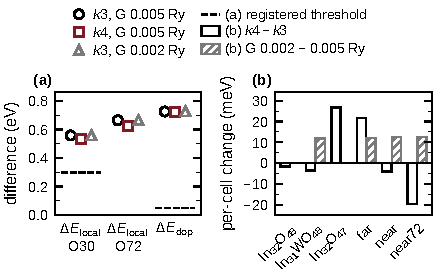
\includegraphics[width=0.97\linewidth]{09_hl_scores}\par
      \raggedright
      \src{(a) Differences on the three settings; dashed: registered thresholds (none for O72). (b) Per-cell change,
        $k4-k3$ (open) and G $0.002-0.005$\,Ry at $k3$ (hatched; 0.0 for the two W-free cells, so no bar). This work,
        PAW-PBE \ninesrclab{computed}; data: f11\_hl\_vacancy.json.}
    \end{column}
    \begin{column}{0.41\textwidth}
      \begin{itemize}
        \item $k3\to k4$ per cell: In$_{32}$O$_{47}$ $+26.8$, far $+21.6$, near $-4.1$, near72 $-19.7$\,meV;
          references In$_{32}$O$_{48}$ $-1.7$, In$_{31}$WO$_{48}$ $-3.5$\,meV \lab{computed}.
        \item $\nineDloc$ = near $-$ far: $-4.1 - 21.6 = -25.7$\,meV. In $\nineDdop$ the changes cancel to
          $-3.4$\,meV, which alone does not show that the energies are converged.
        \item Width 0.002\,Ry: each W cell $+11.7$ to $+12.6$\,meV, the pure cells 0.0\,meV; this cancels in the
          differences.
        \item All six relaxations converged; the near cell needed one restart under the pre-declared rule A28.
      \end{itemize}
    \end{column}
  \end{columns}
  \takeaway{The $k$-mesh rule, not the threshold, leaves $\Delta E_{\mathrm{local}}$ unresolved.}
\end{frame}

% ---------------------------------------------------------------------------------------------------------------------
\begin{frame}{Neither difference is a formation energy at a device Fermi level}
  \ninedense\toggletrue{blx@useprefix}% print "Van de Walle" in the footnote (local to this frame)
  {\small\centering $\displaystyle E^{f}[X^{q}](\EF) = E_{\mathrm{tot}}[X^{q}] - E_{\mathrm{tot}}[\mathrm{host}]
    - \sum\nolimits_i n_i\mu_i + q\,(\EF + E_{\mathrm{VBM}}) + E_{\mathrm{corr}}[X^{q}]$%
    \srefs{VandeWalle2004,Freysoldt2014}\par}
  {\scriptsize\raggedright where $E_{\mathrm{tot}}$: total energy of the cell with defect $X$ (charge $q$) or of the host;
    $n_i$ atoms of chemical potential $\mu_i$ added ($n_i>0$) or removed; $\EF$ measured from the valence-band maximum
    $E_{\mathrm{VBM}}$; $E_{\mathrm{corr}}$: image-charge and potential-alignment correction.\par}
  \vspace{0.3mm}
  \begin{columns}[T,onlytextwidth]
    \begin{column}{0.34\textwidth}
      \centering
      \begin{tikzpicture}[x=1mm,y=1mm,font=\scriptsize]
        % (left) W cell as computed: host band filled to 1.7-1.8 eV above its bottom (schematic; 8 mm per eV)
        \fill[rulegrey!60] plot[domain=-4.76:4.76,samples=40] (\x,{0.6*\x*\x}) -- cycle;
        \draw[line width=0.6pt] plot[domain=-5.8:5.8,samples=50] (\x,{0.6*\x*\x});
        \draw[line width=0.4pt] (-7.5,0) -- (7.5,0) node[right,inner sep=0.5mm]{$\Ec$};
        \draw[dashed,line width=0.5pt] (-7.5,13.6) -- (7.5,13.6) node[right,inner sep=0.5mm]{$\EF$};
        \draw[{Stealth[length=1.2mm]}-{Stealth[length=1.2mm]},line width=0.4pt] (-6.6,0.4) --
          node[left,inner sep=0.5mm,align=right]{1.7--\\1.8\,eV} (-6.6,13.2);
        \draw[-{Stealth[length=1.4mm]},ntumaroon,line width=0.6pt] (4.2,20.2) -- (2.0,14.2);
        \node[anchor=south west,text=ntumaroon,inner sep=0.3mm] at (2.3,20.2) {\nineVO{} electrons};
        \node[anchor=north] at (0,-1.2) {W cell (computed)};
        % (right) device film: E_F below the band edge (inferred, not computed)
        \begin{scope}[xshift=23mm]
          \draw[line width=0.6pt] plot[domain=-5.8:5.8,samples=50] (\x,{0.6*\x*\x});
          \draw[line width=0.4pt] (-6,0) -- (6,0) node[right,inner sep=0.5mm]{$\Ec$};
          \draw[dashed,line width=0.5pt] (-6,-3.6) -- (6,-3.6) node[right,inner sep=0.5mm]{$\EF$};
          \node[anchor=north] at (0,-4.6) {device film};
        \end{scope}
      \end{tikzpicture}\par
      \raggedright
      \src{Schematic; only the 1.7--1.8\,eV filling of the W cell is computed. At device densities $\EF$ lies below
        $\Ec$ \ninesrclab{inferred}.}
    \end{column}
    \begin{column}{0.63\textwidth}
      \begin{itemize}
        \item Band filling: the vacancy electrons enter a band already filled to 1.7--1.8\,eV, so $\nineDdop$ mixes
          filling with chemistry, strain and image terms. At device densities this term would be much smaller
          \lab{inferred}; its sign and size there are not computed.
        \item Cell-limited: the far site is only 6--8\,\AA{} from W and its images, so $\nineDloc$ is a cell-limited
          estimate.
        \item No charged state, $E_{\mathrm{corr}}$ or hybrid functional: no charge-transition level; how deep
          \nineVO{} lies is debated\srefs{Agoston2009,Buckeridge2018,Chatratin2019}.
        \item Crystalline cells; the films are amorphous or nanocrystalline. $\nineDdop$ has the sign that vacancy
          passivation by W\sref[p.~4]{Januar2026} implies, but neither supports nor tests it for the films.
      \end{itemize}
    \end{column}
  \end{columns}
  \takeaway{H-L is a crystalline reference at degenerate filling, not a test of the device films.}
\end{frame}

% 10_multiscale.tex -- Part 10, from first principles to the device. Sources: research_monograph/chapters/
% M12_multiscale.tex (fig:mono-ms-chain, tab:mono-ms-transfer, tab:mono-ms-budget, sec:mono-ms-explain, keyresult),
% M08_c10_campaign.tex (shared parameters, tab:mono-c10-models, tab:mono-c10-hyp H-E/H-J, S1-05 and audit A13),
% M05_confinement_theory.tex (quasi-2-D N_c, Kane dispersion), M09_masses_parameters.tex (tab:mono-mass-tcad deck gaps;
% Kane factor 5.7 % 3-D / 2.5 % quasi-2-D), M15_conclusions.tex (inferred item 3: 44 / 50 / 18 %; tab:concl-plausible
% C2-C4, required measurements), 09_mechanisms_rev.tex (C-V flat-band scaling, optical-gap falsifier, V1 law 0.353 eV),
% appendices/MG_corrections.tex (X4, X5, X12); report_latex_full/chapters/04_derivations_electrostatics.tex and
% 02d_provenance.tex (chi = 4.30 eV from Fan2021, composition-mixing estimate); evidence/derived/multiscale_budget.json;
% evidence/CLAIM_SOURCE_MAP.tsv (M007, C014, C018); evidence/FACT_REGISTRY.tsv (FACT-027, 030, 060, 101-103).
% Figure 10_rigid.pdf: tools/fig_10_multiscale.py (presentation redraw of research_monograph/figures/
% mono_threshold_vs_dft; data: b03_gaps_laws.json, evidence/derived/device_facts.json, multiscale_budget.json).
% No amorphous quantity and no ATLAS result from S2 on.
% Note: frame bodies start with a command, never with a brace group (beamer would read a subtitle).
\partslide{Part 10}{From first principles to the device}

% denser slides: footnotesize bullets, local to the frame in which it is called
\providecommand{\tendense}{\setbeamerfont{itemize/enumerate body}{size=\footnotesize}%
  \setbeamerfont{itemize/enumerate subbody}{size=\footnotesize}}
\providecommand{\tenTop}{\vspace{-4mm}}
\providecommand{\tenNc}{N_{\mathrm{c}}}
\providecommand{\tenNv}{N_{\mathrm{v}}}
\providecommand{\tenQf}{Q_{\mathrm{f}}}
\providecommand{\tenC}[1]{{\tiny\color{inkgrey}\,#1}}
% evidence label inside \src lines (same vocabulary as \lab, at the size of the source text)
\providecommand{\tenL}[1]{{\color{inkgrey}[\textsc{\MakeLowercase{#1}}]}}
\providecommand{\tenData}{Data: Prof.\ M.-H.\ Lee's group, NTU; one device per thickness}
% budget chart (slide 2): centre of row #1; \dy is set inside the picture
\providecommand{\tenyc}[1]{{0.2-(#1-0.5)*\dy}}
% TikZ styles of this section (defined outside the frames: beamer frames do not accept # in their body)
\tikzset{tenbox/.style={draw, line width=0.4pt, align=flush center, font=\scriptsize, inner sep=2.2pt,
    minimum height=13mm, text width=#1}, tenbox/.default=2.5cm,
  tenlow/.style={draw, line width=0.4pt, align=flush left, font=\scriptsize, inner sep=2.2pt, minimum height=10.5mm,
    text width=#1},
  tenarr/.style={-{Stealth[length=1.6mm]}, line width=0.5pt}}

% ---------------------------------------------------------------------------------------------------------------------
\begin{frame}[t]{Only band-edge increments reach the device model}
  \tenTop\tendense
  \par{\centering
  \begin{tikzpicture}[node distance=3mm and 5mm]
    % main chain
    \node[tenbox] (dft) {\textbf{First principles}\\PBE, crystalline (001)\\films 0.46--1.96\,nm\\\lab{computed}};
    \node[tenbox=2.3cm, right=of dft] (law) {\textbf{Thickness laws}\\$\dEc$, $\dEg$, $\Delta m^{*}$\\
      fit3 to 0.70--1.96\,nm\\\lab{fitted}};
    \node[tenbox=3.2cm, right=of law] (deck) {\textbf{Device inputs}\\$\chi = 4.3\,\mathrm{eV} - \dEc(t)$\\
      $\Eg = 3.05\,\mathrm{eV} + \dEg(t)$\\$\tenNc$, $\mu$: $m^{*} = 0.208\,\mzero + \Delta m^{*}$};
    \node[tenbox=3.85cm, right=of deck] (atlas) {\textbf{ATLAS drift--diffusion}\\electrons only, Fermi--Dirac\\
      $\Vthcc$, SS, $I_\mathrm{on}$ compared\\with the measured curves};
    \draw[tenarr] (dft) -- (law);
    \draw[tenarr, ntumaroon, line width=0.9pt] (law) -- (deck);
    \draw[tenarr] (deck) -- (atlas);
    % lower row
    \node[tenlow=5.25cm, dashed, below=2mm of dft.south west, anchor=north west] (notx)
      {\textbf{Computed, not transferred}\\absolute PBE gaps; HSE06 ratio $r = 1.06$--1.11\\
       W donated density $2.7\times10^{21}$\cmcu{} (bulk cells)\\
       $\tenNv = 1.6$--$2.7\times10^{21}$\cmcu; Kane factor in $\tenNc$};
    \node[tenlow=3.0cm, below=2mm of deck] (lit)
      {\textbf{Bulk anchors} (literature)\\$\chi = 4.3$\,eV, $\Eg = 3.05$\,eV\sref{Fan2021}\\
       $m^{*} = 0.208\,\mzero$\sref[p.~225102-1]{Stokey2021}};
    \node[tenlow=4.3cm, below=2mm of atlas.south east, anchor=north east] (fit)
      {\textbf{Not from first principles}\\fitted: $\Delta V_0$ ($\tenQf$), $\mu_\infty$, $\ell$, $N_{\mathrm{s}}$,
       $W_{\mathrm{TA}}$\\fitted in model V1, fixed in C10: donors $2.5\times10^{17}$\cmcu\\
       assumed: $\tenNv$, deep and interface traps};
    \draw[tenarr, dashed] (dft.south) -- (dft.south |- notx.north);
    \draw[tenarr] (lit) -- (deck);
    \draw[tenarr] (atlas.south |- fit.north) -- (atlas.south);
  \end{tikzpicture}\par}
  \src{C10 decks: fit3 laws incl.\ the polar 0.695\,nm film (caveat: not in the primary $\dEc$ fit); quasi-2-D
    $\tenNc$ at 2.0\,nm (one subband, $E_2 - E_1 = 0.72$\,eV \tenL{computed}); 4.3\,eV: composition-mixing estimate,
    3.05\,eV: optical gap, both of another sputtered IWO device; $m^{*}$ measured; shared fits ($\tenQf$: front charge;
    $\mu_\infty$, $\ell$: mobility law; $N_{\mathrm{s}}$, $W_{\mathrm{TA}}$: tail density, width). W fully ionised
    \tenL{inferred}. Assumed: $\tHH$ = device thickness; OH-terminated crystalline films stand for the device films;
    traps shift rigidly with $\Ec$.}
  \vspace{-0.5mm}
  \begin{itemize}
    \item Effectively one independent law is transferred: the mass increase follows from $\dEc$ by the Kane
      relation\sref{Kane1957} within 1\,\% at 1.962\,nm (10\,\% at 0.930\,nm) \lab{derived}; $\dEg$ enters only $n_i$;
      6.3 and 13.2\,nm are extrapolated.
  \end{itemize}
  \takeaway{Effectively one first-principles law, $\dEc(t)$ (fitted), and an $\tenNc$ convention carry thickness.}
\end{frame}

% ---------------------------------------------------------------------------------------------------------------------
\begin{frame}[t]{A convention, not the crystal, leads the DFT-related budget}
  \tenTop\tendense
  \par{\centering
  \begin{tikzpicture}[x=1cm,y=1cm,font=\scriptsize]
    % columns: source (0 .. 5.6 cm), value (5.7 .. 8.4 cm), log axis 1 .. 1000 mV (8.6 .. 13.55 cm, 1.65 cm/decade)
    \def\ax{8.6}\def\dec{1.65}\def\dy{0.4}\def\nr{6}%
    % row i: centre at 0.2-(i-0.5)*dy, rule below at 0.2-i*dy; the log axis replaces the last rule
    \def\yb{{0.2-\nr*\dy}}
    % reference band: the three 6.3 nm misses, 230 .. 370 mV; dashed: measured 2.0 -> 13.2 nm step, 579 mV
    \fill[black!10] ({\ax+\dec*log10(230)},0.2) rectangle ({\ax+\dec*log10(370)},\yb);
    \draw[dashed, line width=0.5pt] ({\ax+\dec*log10(579)},0.2) -- ({\ax+\dec*log10(579)},\yb);
    % header
    \node[anchor=west, font=\scriptsize\bfseries] at (0,0.42) {Input choice (2.0\,nm unless stated)};
    \node[anchor=west, font=\scriptsize\bfseries] at (5.7,0.42) {Effect on $\Vthcc$ (mV)};
    % key to the two reference marks, right-aligned above the axis area
    \node[anchor=east, inner sep=1pt] (tenk2) at ({\ax+3*\dec},0.42) {2.0--13.2\,nm step\sref{Januar2026}};
    \draw[dashed, line width=0.5pt] ([xshift=-1.2mm]tenk2.west) -- ++(-4.5mm,0);
    \node[anchor=east, inner sep=1pt] (tenk1) at ([xshift=-7.2mm]tenk2.west) {6.3\,nm misses};
    \fill[black!10] ([xshift=-1.2mm, yshift=-1mm]tenk1.west) rectangle ++(-3.2mm,2mm);
    \draw[line width=0.6pt] (0,0.2) -- ({\ax+3*\dec},0.2);
    % rows
    \foreach \i/\lbl/\val in {
        1/{$\tenNc$ convention: quasi-2-D vs 3-D}/{$+142$ (ATLAS, stage S1)},
        2/{Thickness definition, $\pm0.2$\,nm}/{$\approx\pm40$},
        3/{HSE06 ratio on $\dEc$, $r = 1.06$--1.11}/{$+16$ to $+29$},
        4/{$\dEc$ fit options, 0.273--0.289\,eV}/{$\pm8$},
        5/{Kane factor in 3-D $\tenNc$ ($+5.7$\,\%)}/{1.4 free; 5 with tail},
        6/{Mass fit basis ($\pm3$\,\% in $m^{*}$, 3-D $\tenNc$)}/{1 free; 4 with tail}} {
      \node[anchor=west] at (0,\tenyc{\i}) {\lbl};
      \node[anchor=west] at (5.7,\tenyc{\i}) {\val};
      \draw[rulegrey, line width=0.3pt] (0,{0.2-\i*\dy}) -- (\ax,{0.2-\i*\dy});
      \ifnum\i<\nr \draw[rulegrey, line width=0.3pt] (\ax,{0.2-\i*\dy}) -- ({\ax+3*\dec},{0.2-\i*\dy});\fi
    }
    % markers (values: evidence/derived/multiscale_budget.json; M12 tab:mono-ms-budget)
    \fill[ntumaroon] ({\ax+\dec*log10(142)},\tenyc{1}) circle (0.075);
    \fill ({\ax+\dec*log10(40.4)},\tenyc{2}) circle (0.06);
    \draw[line width=1.6pt] ({\ax+\dec*log10(16.4)},\tenyc{3}) -- ({\ax+\dec*log10(29.3)},\tenyc{3});
    \fill ({\ax+\dec*log10(7.65)},\tenyc{4}) circle (0.06);
    \draw[line width=0.5pt] ({\ax+\dec*log10(1.43)},\tenyc{5}) -- ({\ax+\dec*log10(5.02)},\tenyc{5});
    \draw[fill=white, line width=0.5pt] ({\ax+\dec*log10(1.43)},\tenyc{5}) circle (0.06);
    \fill ({\ax+\dec*log10(5.02)},\tenyc{5}) circle (0.06);
    \draw[line width=0.5pt] ({\ax+\dec*log10(1.15)},\tenyc{6}) -- ({\ax+\dec*log10(4.01)},\tenyc{6});
    \draw[fill=white, line width=0.5pt] ({\ax+\dec*log10(1.15)},\tenyc{6}) circle (0.06);
    \fill ({\ax+\dec*log10(4.01)},\tenyc{6}) circle (0.06);
    % log axis
    \draw[line width=0.5pt] (\ax,\yb) -- ({\ax+3*\dec},\yb);
    \foreach \e/\t in {0/1,1/10,2/100,3/1000} {
      \draw ({\ax+\e*\dec},\yb) -- ({\ax+\e*\dec},{0.2-\nr*\dy+0.08});
      \node[anchor=north, inner sep=1.5pt] at ({\ax+\e*\dec},\yb) {\t};
    }
    \foreach \e in {0,1,2} {\foreach \m in {2,3,4,5,6,7,8,9} {
      \draw ({\ax+\e*\dec+\dec*log10(\m)},\yb) -- ({\ax+\e*\dec+\dec*log10(\m)},{0.2-\nr*\dy+0.04});}}
    \node[anchor=north] at ({\ax+1.5*\dec},{0.2-\nr*\dy-0.28}) {$|\Delta\Vthcc|$ (mV, log scale)};
  \end{tikzpicture}\par}
  \src{Row 1: ATLAS run S1-05, seen before register revision 2 \tenL{computed}; rows 2--6 \tenL{derived} (laws, audit
    A13); rows 5--6 in the 3-D $\tenNc$ form; open: free carriers, filled: with tail filling. Band: 0.23--0.37\,V;
    dashed: measured 2.0--13.2\,nm step, 0.579\,V. Crystalline vs amorphous: unknown, H-K sealed (Part 11). \tenData.}
  \vspace{-0.5mm}
  \begin{itemize}
    \item In the model, $\dEc$ shifts $\Vthcc$ one-to-one by construction (traps move with $\Ec$; test H-E sealed); mass
      and $\tenNc$ act through the statistics, amplified about 3.5 times by the 40\,meV tail (registered audit A13;
      Part 4).
  \end{itemize}
  \takeaway{Ranking: $\tenNc$ convention, thickness definition, functional; the rest is minor.}
\end{frame}

% ---------------------------------------------------------------------------------------------------------------------
\begin{frame}[t]{Rigid $\dEc$ gives 44\,\% of the 2.0--13.2\,nm step, 0.2\,V off at 6.3\,nm}
  \tenTop\tendense
  \begin{columns}[T,onlytextwidth]
    \begin{column}{0.43\textwidth}
      \centering
      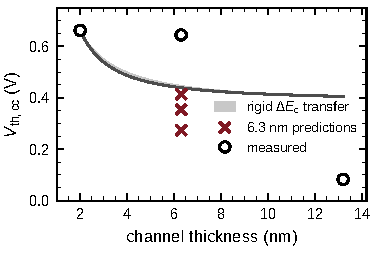
\includegraphics[width=\linewidth]{10_rigid}
      \raggedright
      \src{Measured $\Vthcc$ (circles) against $\Vthcc(2.0) + [\dEc(t) - \dEc(2.0)]/q$ (band: four fit options; line:
        two-point fit). Crosses: failed 6.3\,nm predictions (C014). Rigid 1:1 transfer, not a model run \tenL{derived}.
        \tenData.}
    \end{column}
    \begin{column}{0.54\textwidth}
      \begingroup\scriptsize
      \setlength{\tabcolsep}{6pt}
      \renewcommand{\arraystretch}{0.98}
      \begin{tabular}{@{}l c c@{}}
        \toprule
        $\Delta\Vthcc$ (V) & rigid $\dEc$ & measured\sref{Januar2026} \\
        \midrule
        2.0 $\to$ 13.2\,nm & $-0.257$ & $-0.579$ \\
        2.0 $\to$ 6.3\,nm & $-0.21$ to $-0.22$ & $-0.018$ \\
        \midrule
        6.3\,nm misses & \multicolumn{2}{c}{$-0.29$, $-0.37$, $-0.23$ \lab{falsified}} \\
        \bottomrule
      \end{tabular}\par\endgroup
      \src{Rigid: fit-option spread below 2\,meV (2.0--13.2\,nm). Misses: model V1 run 0014; model V2 P, E, run 0060
        (Part 4). Claims M007 \tenL{derived}, C018. Causes: Part 12.}
      \begin{itemize}
        \item 2.0--13.2\,nm step: the rigid shift is 44\,\% of it \lab{derived}; other model inputs partly cancel
          it (audit A13 forecast $\approx$18\,\%; earlier calibration $\approx$50\,\%).
        \item 2.0 to 6.3\,nm: the rigid shift puts 6.3\,nm $\approx$0.2\,V too low, like all three misses. No cause
          assigned: the device acts as if much thinner, or as if charge raised $\Vthcc$ by 0.2\,V.
        \item Model V2 vs model V1, like with like: this work's DFT laws shrink the miss by only $\approx$0.04\,V
          \lab{computed}.
      \end{itemize}
    \end{column}
  \end{columns}
  \takeaway{Confinement alone does not carry the 2.0--13.2\,nm step \lab{inferred}.}
\end{frame}

% ---------------------------------------------------------------------------------------------------------------------
\begin{frame}[t]{Three probes and device statistics can separate the inputs}
  \tenTop\tendense
  \begin{itemize}
    \item In transfer curves, gate work function, bulk affinity, a uniform fixed charge and $\dEc$ act as one number
      per film \lab{derived}; a shared $\Delta V_0$ for three films (registered campaign, sealed) is the first test
      the computed inputs can fail.
  \end{itemize}
  \vspace{0.5mm}
  \begingroup\scriptsize
  \setlength{\tabcolsep}{4pt}
  \renewcommand{\arraystretch}{1.1}
  \begin{tabularx}{\textwidth}{@{}>{\raggedright\arraybackslash}p{3.2cm}>{\raggedright\arraybackslash}p{4.0cm}
      >{\raggedright\arraybackslash}X@{}}
    \toprule
    Measurement against $t$ & What it separates & Value or falsifier at stake \\
    \midrule
    C--V flat band $V_{\mathrm{FB}}(t)$ & charges by their scaling: front sheet $t^0$, volume $t$ and $t^2$, back sheet
      $t/\varepsilon_s$ &
      donor or positive-charge step at 13.2\,nm: falsified if $V_{\mathrm{FB}}(t)$ is flat within 50\,mV \\
      \addlinespace[1pt]
    Optical gap & confinement, a band-edge property, from charge &
      deck gaps 3.38, 3.12, 3.08\,eV at 2.0, 6.3, 13.2\,nm; confinement falsified if the 2.0--13.2\,nm shift is
      below 0.1\,eV \\ \addlinespace[1pt]
    Photoemission offsets (UPS, IPES), Kelvin probe & $\chi(t)$ and work function directly: $\dEc$ apart from
      $\tenQf$ &
      this work's DFT: $\dEc(2.0) = 0.273$--0.289\,eV over fit options (model V1 law, fitted to published slab DFT:
      0.353\,eV); $\times1.06$--1.11 with HSE06 \\ \addlinespace[1pt]
    $\ge 10$ devices per thickness, one run, dual sweeps & device spread from a film property &
      device-specific 6.3\,nm offset: falsified if the mean is $\ge 0.2$\,V off a smooth law with
      $\sigma(\Vth) < 0.1$\,V \\
    \bottomrule
  \end{tabularx}\par\endgroup
  \src{Right column: the monograph's plausible-mechanism conjectures with their falsifiers; campaign
    C10; claim C018. Deck gaps: PBE increments on the 3.05\,eV optical anchor (first slide of this part) \tenL{derived};
    $\dEc$: fit3, C10 decks. $\tenQf$: front fixed charge; $\varepsilon_s$:
    channel permittivity. None of these measurements exists yet for the present films.}
  \takeaway{Band-edge and charge probes can isolate the shift; replicates test the 6.3\,nm offset.}
\end{frame}

% 11_amorphous.tex -- Part 11, amorphous films: the registered protocol. Sources: research_monograph/chapters/
% M11_amorphous_protocol.tex (sec:mono-am-why, -scope, -mace, -slabs, tab:mono-am-cells, sec:mono-am-mlval,
% tab:mono-am-mace, -relax, -smearing, -restart, -final, -defs, sec:mono-am-hn, tab:mono-am-hn-controls,
% prop:mono-hn, sec:mono-am-a37, sec:mono-am-release); M06_defect_theory.tex (sec:mono-defect-pr,
% tab:mono-defect-pr); M03_literature_materials.tex (sec:mono-lit-amorph); appendices/MG_corrections.tex (X8, X13);
% evidence/CLAIM_SOURCE_MAP.tsv (M001, M005, C034-C037); evidence/FACT_REGISTRY.tsv (FACT-014, FACT-070..073,
% FACT-081); evidence/derived/defect_estimates.json (PR_support).
% Blind rules: protocol facts and force-only checks only; no electronic quantity of any aIO_* / aIWO_* cell;
% per-cell outcomes are \sealed{}. No figure of amorphous electronic structure exists or is used.
% Note: frame bodies start with a command, never with a brace group (beamer would read a subtitle).
\providecommand{\elevenfext}{f_{\mathrm{ext}}}
\providecommand{\elevenflocW}{f_{\mathrm{locW}}}
\providecommand{\elevenDW}{\Delta_{\mathrm{W}}}
\providecommand{\elevenNex}{N_{\mathrm{ex}}}
\providecommand{\elevenNeff}{N_{\mathrm{eff}}}
\providecommand{\elevenEh}{E_{\mathrm{host}}}
\providecommand{\elevenAng}{\mbox{\AA}}
\providecommand{\elevenRyb}{\,Ry/bohr}
% denser slides: footnotesize bullets, local to the frame in which it is called
\providecommand{\elevendense}{\setbeamerfont{itemize/enumerate body}{size=\footnotesize}%
  \setbeamerfont{itemize/enumerate subbody}{size=\footnotesize}}

\partslide{Part 11}{Amorphous films: the registered protocol}

% ---------------------------------------------------------------------------------------------------------------------
\begin{frame}{The channels are disordered; all DFT so far is crystalline}
  \elevendense
  \begin{columns}[T,onlytextwidth]
    \begin{column}{0.56\textwidth}
      \begin{itemize}
        \item The channels are sputtered, largely amorphous or nanocrystalline: HRTEM shows no long-range
          crystallinity\sref[p.~2]{Januar2026}.
        \item Amorphous \InO{} keeps edge- and corner-sharing InO$_x$ polyhedra whose connectivity is linked to
          transport\sref{Buchholz2014}; its s-like conduction band survives disorder\sref{Medvedeva2017}.
        \item Test H-N: does W still put its electron into an extended host state at 0.7\,nm? Confinement, weaker
          screening, surfaces (every atom within about 0.35\,nm of one) and 2-D disorder could prevent it
          \lab{theory}.
        \item Below a mobility edge states are localised; in 2-D weak disorder localises all states on long
          scales\srefs{Anderson1958,Mott1969,Abrahams1979}. A 1--3\,nm cell sees only few-atom localisation, the
          scale of a deep, d-like W trap.
      \end{itemize}
    \end{column}
    \begin{column}{0.40\textwidth}
      \centering
      \begin{tikzpicture}[x=1mm,y=1mm,font=\scriptsize,line width=0.5pt]
        % (top) periodic supercell: three images of one cell of lateral size L
        \foreach \c in {0,16,32,48} {\draw[rulegrey,dashed] (\c,0) -- (\c,8);}
        \draw (0,0) -- (48,0);
        \draw[line width=0.7pt] plot[domain=0:48,samples=220]
          (\x,{7*exp(-((\x-8)^2)/1.4)+7*exp(-((\x-24)^2)/1.4)+7*exp(-((\x-40)^2)/1.4)});
        \draw[line width=0.7pt,inkgrey] (0,1.8) -- (48,1.8);
        \node[anchor=west,inner sep=0.6mm] at (9.4,6.0) {localised};
        \node[anchor=west,inner sep=0.6mm,text=inkgrey] at (25.4,3.1) {extended};
        \draw[{Stealth[length=1.2mm]}-{Stealth[length=1.2mm]}] (16,-1.4) -- node[below,inner sep=0.5mm]{cell, $L = 1$--3\,nm} (32,-1.4);
        \node[anchor=south west,inner sep=0] at (0,8.6) {supercell, periodic images};
        % (bottom) the same disorder in an infinite film: a state localised on a length xi >> L
        \begin{scope}[yshift=-19mm]
          \draw (0,0) -- (48,0);
          \draw[line width=0.7pt] plot[domain=0:48,samples=120] (\x,{7*exp(-abs(\x-20)/10)});
          \draw[ntumaroon,line width=0.7pt] (17.8,7.9) -- (17.8,8.9) -- (22.2,8.9) -- (22.2,7.9);
          \node[anchor=south,text=ntumaroon,inner sep=0.5mm] at (20,8.9) {$L$};
          \draw[{Stealth[length=1.2mm]}-{Stealth[length=1.2mm]}] (10,-1.4) -- node[below,inner sep=0.5mm]{$\xi$ = tens of nm} (30,-1.4);
          \node[anchor=south west,align=left,inner sep=0] at (31.0,3.4) {flat within\\one cell: read\\as extended};
          \node[anchor=south west,inner sep=0] at (0,8.6) {film};
        \end{scope}
      \end{tikzpicture}\par
      \raggedright
      \src{Schematic of $|\psi|^2$ along the film, not to scale. Top: a 1--3\,nm periodic cell separates a
        few-atom state from an extended one. Bottom: a state localised on tens of nm is nearly flat across one
        cell, so the cell reads it as extended.}
    \end{column}
  \end{columns}
\end{frame}

% ---------------------------------------------------------------------------------------------------------------------
\begin{frame}{Every cell goes from ML melt--quench to a certified read-out}
  \elevendense
  \begingroup\centering
  \begin{tikzpicture}[x=1mm,y=1mm,font=\scriptsize,
      st/.style={draw,line width=0.45pt,align=center,text width=17.6mm,minimum height=8.4mm,inner sep=0.8mm},
      ar/.style={-{Stealth[length=1.6mm]},line width=0.5pt}]
    \node[st] (a) at (11,0)   {MACE-MPA-0\\melt--quench};
    \node[st] (b) at (34.6,0) {force check\\against PBE};
    \node[st] (c) at (58.2,0) {PBE relaxation\\(GPU)};
    \node[st] (d) at (81.8,0) {final SCF and\\projections (CPU)};
    \node[st] (e) at (105.4,0) {frozen read-out\\and certificate};
    \node[st,dashed] (f) at (129,0) {release\\(D-43)};
    \foreach \u/\v in {a/b,b/c,c/d,d/e,e/f} {\draw[ar] (\u) -- (\v);}
    \node[anchor=north,text=ntumaroon,inner sep=0.8mm] at (b.south) {failed at W};
    \node[anchor=north,text=inkgrey,inner sep=0.8mm] at (f.south) {sealed};
  \end{tikzpicture}\par\endgroup
  \vspace{0.6mm}
  \begin{columns}[T,onlytextwidth]
    \begin{column}{0.49\textwidth}
      {\footnotesize\textbf{Melt--quench}, MACE-MPA-0 ``medium''\srefs{Batatia2022,Batatia2023}\par}
      \begin{itemize}
        \item Langevin, 1\,fs, friction 0.01\,fs$^{-1}$: 3000\,K for 6\,ps, quench to 300\,K over 9\,ps, hold
          2\,ps; open the vacuum gap, 800\,K for 3\,ps, cool over 3\,ps; relax to 0.05\,eV/\elevenAng, passivate,
          relax again.
        \item Gate on density, bond lengths and coordination; a failed structure is replaced by the next seed
          (three were), thresholds unchanged.
        \item 23\,ps is about $10^{14}$\,K/s: a network of the right composition and density, not a model of the
          sputtered film.
      \end{itemize}
    \end{column}
    \begin{column}{0.48\textwidth}
      {\footnotesize\textbf{PBE relaxation and final SCF}\par}
      \begin{itemize}
        \item 60/480\,Ry; BFGS to $10^{-3}$\elevenRyb{} and $10^{-4}$\,Ry; $2{\times}2{\times}1$ $k$ grid; dipole
          correction. Converged only on ``bfgs converged'' (A19).
        \item Final SCF at 71/568\,Ry with $1.3\times$ the occupied bands, then L\"owdin projections.
        \item The frozen read-out (D-32; 221 tests) must first reproduce two crystal values: a 3\,\% W-5d share and
          $\dEc = 0.281$\,eV at 2\,nm.
      \end{itemize}
    \end{column}
  \end{columns}
\end{frame}

% ---------------------------------------------------------------------------------------------------------------------
\begin{frame}{Six W cells span bulk to 0.7\,nm at one W volume density}
  \elevendense
  \begingroup\scriptsize
  \setlength{\tabcolsep}{5pt}
  \renewcommand{\arraystretch}{1.06}
  \begin{tabularx}{\textwidth}{@{}l l l r l >{\raggedright\arraybackslash}X@{}}
    \toprule
    $t_{\mathrm{eq}}$ & W-doped cell & composition & $N$ & undoped partner & role in H-N \\
    \midrule
    bulk   & \cell{aIWO_bulk_s1} & In$_{49}$W$_1$O$_{76}$, no surface & 126 & \cell{aIO_bulk_s1} & bulk point \\
    2.0\,nm & \cell{aIWO_2p0_s1} & In$_{98}$W$_2$ film, OH/H & 270 & \cell{aIO_2p0_s1} (268) & thick endpoint, seed 1 \\
    2.0\,nm & \cell{aIWO_2p0_s2} & In$_{98}$W$_2$O$_{156}$H$_8$ & 264 & \cell{aIO_2p0_s2} & thick endpoint, seed 2 \\
    1.0\,nm & \cell{aIWO_1p0_s1} & In$_{49}$W$_1$O$_{80}$H$_8$ & 138 & \cell{aIO_1p0_s1} (134) & intermediate \\
    0.8\,nm & \cell{aIWO_0p8_s2} & In$_{49}$W$_1$O$_{76}$ film, OH/H & 147 & \cell{aIO_0p8_s1} & intermediate \\
    0.7\,nm & \cell{aIWO_0p7_s1} & In$_{49}$W$_1$O$_{83}$H$_{14}$ & 147 & \cell{aIO_0p7_s1} & thin decisive endpoint \\
    \bottomrule
  \end{tabularx}\par\endgroup
  \src{$N$: atoms (register and claims ledger); one melt--quench sample per name. 1.5\,nm cut under the budget rule.
    Controls: a compensated 2.0\,nm cell (In$_{98}$W$_2$O$_{160}$H$_{14}$, 274 atoms, no excess electron), bare
    surfaces at 2.0 and 0.7\,nm, \AlO{} and \HfO{} interfaces. Slab rules registered before any ML or DFT result
    (D-14). Structural facts only.}
  \vspace{1.2mm}
  \begin{columns}[T,onlytextwidth]
    \begin{column}{0.49\textwidth}
      \begin{itemize}
        \item W/(In+W) $= 2.0$\,\%. Each W brings one extra O, so one excess electron per W (W$^{6+}$ for In$^{3+}$
          gives three, the O$^{2-}$ takes two): about $6\times10^{20}$\cmcu.
        \item In-plane edge $\ge 12.5$\,\elevenAng{} at 7.0\,g/cm$^3$: the same W density at every thickness.
      \end{itemize}
    \end{column}
    \begin{column}{0.48\textwidth}
      \begin{itemize}
        \item $t_{\mathrm{eq}}$ = film mass / (7.0\,g/cm$^3$ $\times$ area), not the H--H thickness of Parts 6--8.
        \item OH and H in pairs (electron count unchanged); 18\,\elevenAng{} vacuum with a dipole
          correction\sref{Bengtsson1999}.
      \end{itemize}
    \end{column}
  \end{columns}
\end{frame}

% ---------------------------------------------------------------------------------------------------------------------
\begin{frame}{The ML potential fails at W; its structures only seed DFT}
  \elevendense
  \begin{columns}[T,onlytextwidth]
    \begin{column}{0.59\textwidth}
      \begingroup\scriptsize
      \setlength{\tabcolsep}{2.3pt}
      \renewcommand{\arraystretch}{1.08}
      \begin{tabular}{@{}l l c c c@{}}
        \toprule
        structure & frame & RMSE & MAE & RMSE$_{\mathrm{W1}}$ \\
        \multicolumn{2}{@{}l}{\color{inkgrey}registered limit (eV/\elevenAng)} & {\color{inkgrey}0.15} &
          {\color{inkgrey}0.10} & {\color{inkgrey}0.25} \\
        \midrule
        a-\InO, bulk & quenched / final & 0.068 / 0.065 & 0.052 / 0.049 & -- \\
        a-IWO, bulk & quenched / final & 0.121 / 0.122 & 0.068 / 0.068 & \textbf{0.434 / 0.449} \\
        a-IWO, 0.7\,nm & final & \textbf{0.206} & \textbf{0.110} & \textbf{0.815} \\
        melt frame & not scored & 0.311 & 0.171 & 1.108 \\
        \bottomrule
      \end{tabular}\par\endgroup
      \src{MACE forces against PBE single points (QE 7.5, MV 0.01\,Ry) on the same geometries; W1: W and its
        first-shell O; bold: limit exceeded. Comparator frozen before any output was read. C037 \lab{computed}.}
    \end{column}
    \begin{column}{0.38\textwidth}
      \begin{itemize}
        \item Verdict: \textbf{failed overall}. 71--75\,\% of the squared error sits in the W first shell (7 atoms);
          outside it the RMSE is 0.063--0.066 (bulk), 0.107\,eV/\elevenAng{} (0.7\,nm).
        \item Registered consequence: DFT starting points, not validated amorphous models; no ML-stage structural
          statistic is reported (X8).
      \end{itemize}
    \end{column}
  \end{columns}
  \vspace{1.6mm}
  \begingroup\scriptsize
  \setlength{\tabcolsep}{4pt}
  \renewcommand{\arraystretch}{1.08}
  \begin{tabularx}{\textwidth}{@{}l l l l >{\raggedright\arraybackslash}X@{}}
    \toprule
    numerical control (claim) & cell & change & tolerance & result \\
    \midrule
    smearing MV $\to$ Gaussian (C034) & \cell{aIWO_1p0_s1} & max $|\Delta F| = \num{2.4e-4}$\elevenRyb
      & \num{1e-3}\elevenRyb & pass (a screen) \\
    split species labels (C035) & \cell{aIO_1p0_s1} & $|\Delta E| = \num{1e-8}$\,Ry & \num{1e-5}\,Ry
      & pass \\
    fresh restart, same input (C036) & \cell{aIWO_0p8_s2} & max $|\Delta F| = \num{4.99e-3}$\elevenRyb & --
      & not reproduced; cause open \\
    \bottomrule
  \end{tabularx}\par\endgroup
  \src{PAW-PBE, one geometry each \lab{computed}. Since C036, every rescue-route cell needs a restart gate and a
    qualification SCF ($10^{-5}$\,Ry, $10^{-3}$\elevenRyb); otherwise its relaxation is exploratory.}
\end{frame}

% ---------------------------------------------------------------------------------------------------------------------
\begin{frame}{H-N classifies each W cell by frozen observables}
  \elevendense
  \begin{columns}[T,onlytextwidth]
    \begin{column}{0.50\textwidth}
      {\footnotesize Final SCF, bands $n > N_v$, $\elevenNex = n_{\mathrm{W}}$ excess electrons:\par}
      \vspace{-1.6mm}
      {\footnotesize
      \begin{align*}
        \elevenfext &= \tfrac{1}{\elevenNex}\textstyle\sum f_{n\mathbf{k}}w_{\mathbf{k}}\,
          \mathbf{1}\!\left[\PRn \ge 0.20,\ \varepsilon_{n\mathbf{k}} \ge \elevenEh\right]\\
        \elevenflocW &= \tfrac{1}{\elevenNex}\textstyle\sum f_{n\mathbf{k}}w_{\mathbf{k}}\,
          \mathbf{1}\!\left[\PRn \le 0.05,\ p_{\mathrm{W5d}} \ge 0.30\right]\\
        \elevenDW &= \min\{\varepsilon_{n\mathbf{k}} : p_{\mathrm{W5d}} \ge 0.30\} - \elevenEh
      \end{align*}\par}
      \vspace{-1.2mm}
      {\scriptsize $f, w$: occupation, $k$ weight; $p_{\mathrm{W5d}}$: W-5d weight; $\elevenEh$: host edge, lowest
        state with $\PRn \ge 0.20$ and interior weight (W weight not used).\par}
      \vspace{1.0mm}
      {\footnotesize Participation ratio, L\"owdin atom weights $p_i$, $N$ atoms\srefs{BellDean1970,Thouless1974}:\par}
      \vspace{-1.6mm}
      {\footnotesize\[ \PRn = \frac{1}{N\sum_i p_i^2}, \qquad \elevenNeff = N\,\PRn \]\par}
      \vspace{-1.2mm}
      {\scriptsize Equal weight on $M$ atoms: $\PRn = M/N$. Extended $\PRn \ge 0.20$, localised $\PRn \le 0.05$
        (absolute); $\elevenNeff$ reported for every state.\par}
    \end{column}
    \begin{column}{0.46\textwidth}
      \begingroup\scriptsize
      \renewcommand{\arraystretch}{1.12}
      \begin{tabularx}{\linewidth}{@{}l >{\raggedright\arraybackslash}X@{}}
        \toprule
        class & rule, per W cell \\
        \midrule
        \textsc{donor} & $\elevenfext \ge 0.80$, $\elevenDW > 0.3$\,eV, $\elevenflocW < 0.10$ \\
        \textsc{ecb} & $\elevenfext < 0.50$ or $\elevenflocW \ge 0.50$ \\
        \textsc{partial} & otherwise \\
        \textsc{unresolved} & completeness $< 0.90$, electron count off $> 0.02$\,e, too few bands, qualification
          pending \\
        \bottomrule
      \end{tabularx}\par\endgroup
      \src{\textsc{ecb}: extended-carrier efficacy breakdown.}
      \begin{itemize}
        \item \textsc{ecb} need not mean W stopped donating: a host or surface trap may hold the electron.
          W-centred needs $\ge 30$\,\% trap weight on W and its shell.
        \item Neutral PBE shows where the electron goes in the cell, not a charge-transition
          level\srefs{Freysoldt2014,Lany2008}. PBE favours delocalisation.
      \end{itemize}
    \end{column}
  \end{columns}
  \vspace{0.3mm}
  \src{Register section 1 (A16, A24) and amendment A27 (2026-10-11, 09:09Z), before any slab electronic result. H-N
    is exploratory: read-out rules frozen, forecasts not scored.}
\end{frame}

% ---------------------------------------------------------------------------------------------------------------------
\begin{frame}{Absolute PR thresholds mean different supports per cell}
  \elevendense
  \begin{columns}[T,onlytextwidth]
    \begin{column}{0.50\textwidth}
      \begingroup\footnotesize
      \setlength{\tabcolsep}{4.5pt}
      \renewcommand{\arraystretch}{1.15}
      \begin{tabular}{@{}l r c c c@{}}
        \toprule
        W cell & $N$ & localised & extended & $\PRn$ at \\
               &     & $M \le 0.05N$ & $M \ge 0.20N$ & $M = 7$ \\
        \midrule
        bulk & 126 & 6.3 & 25.2 & 0.056 \\
        1.0\,nm & 138 & 6.9 & 27.6 & 0.051 \\
        0.8, 0.7\,nm & 147 & 7.4 & 29.4 & 0.048 \\
        2.0\,nm, s2 & 264 & 13.2 & 52.8 & 0.027 \\
        2.0\,nm, s1 & 270 & 13.5 & 54.0 & 0.026 \\
        \bottomrule
      \end{tabular}\par\endgroup
      \src{Support size $M$ in atoms implied by the frozen thresholds; $M = 7$: weight spread evenly over W and its
        six first-shell O. From the rule and the atom counts only \lab{derived} (M005).}
    \end{column}
    \begin{column}{0.46\textwidth}
      \begin{itemize}
        \item For a fixed support of $M$ atoms, $\PRn = M/N$ falls as $1/N$: one absolute threshold is a different
          support size in each cell.
        \item An even W + 6\,O state ($M = 7$) is localised at 0.7, 0.8 and 2.0\,nm, but intermediate in bulk and at
          1.0\,nm \lab{derived}.
        \item More concentrated states are localised everywhere: half the weight on W, the rest on six O, gives
          $\elevenNeff = 3.4$.
        \item The rule is unchanged; the table is a reading aid for the released results.
      \end{itemize}
    \end{column}
  \end{columns}
  \takeaway{Localised means at most about 6--7 atoms in bulk and thin cells, about 13 at 2.0\,nm.}
\end{frame}

% ---------------------------------------------------------------------------------------------------------------------
\begin{frame}{By its frozen rules, H-N cannot return a crossover verdict}
  \elevendense
  \begin{columns}[T,onlytextwidth]
    \begin{column}{0.54\textwidth}
      \begingroup\scriptsize
      \setlength{\tabcolsep}{3.4pt}
      \renewcommand{\arraystretch}{1.08}
      \begin{tabularx}{\linewidth}{@{}l c c >{\raggedright\arraybackslash}X@{}}
        \toprule
        control & 2.0\,nm & 0.7\,nm & what it tests \\
        \midrule
        C1 paired substitution & -- & req. & W + O in undoped parent \\
        C2 directional dilution & -- & cut & W halved along one axis \\
        C3 occupation width & req. & req. & 0.001\,Ry reference \\
        C4 Gaussian polish & req. & req. & MV geometry re-relaxed \\
        C5 hybrid functional & -- & cut & HSE06, fixed geometry \\
        C6 spin & req. & req. & nspin = 2, two starts \\
        \bottomrule
      \end{tabularx}\par\endgroup
      \src{As registered (A27) and amended (A37: C2, C5 cut).}
      \vspace{0.4mm}
      \begin{itemize}
        \item \textsc{crossover}: bulk and \emph{both} 2.0\,nm seeds \textsc{donor}, 0.7\,nm \textsc{ecb}, controls
          passing at both endpoints.
        \item \textsc{no crossover}: \textsc{donor} at bulk, 2.0, 1.0, 0.8 and 0.7\,nm, all resolved, controls
          passing at 0.7\,nm.
      \end{itemize}
    \end{column}
    \begin{column}{0.42\textwidth}
      {\footnotesize\textbf{Proposition} (M001). Under the frozen rules and A37, the registered H-N outcome is
        \textsc{unresolved} in every branch.\par}
      \vspace{1.2mm}
      {\footnotesize\textit{Proof.} Both verdicts need both 2.0\,nm seeds \textsc{donor} with C4. Seed 2
        (\cell{aIWO_2p0_s2}) never converged in its only MV segment and continues on the one-attempt Gaussian route (A36): it has no MV
        parent to polish, so C4 cannot be met. No other 2.0\,nm W seed exists; an amendment admitting a native-Gaussian seed
        was declined as result-exposed (A36 erratum). A37 sets the outcome to \textsc{unresolved}; per-cell classes stay
        intact.\hfill$\square$\par}
      \vspace{1.0mm}
      {\scriptsize\color{inkgrey} A37: 2026-10-13, 00:10Z (D-42), before any H-N class was computed; no sealed value
        is used \lab{derived}.\par}
    \end{column}
  \end{columns}
  \takeaway{Neither ``W stops donating below a critical thickness'' nor its opposite can be registered.}
\end{frame}

% ---------------------------------------------------------------------------------------------------------------------
\begin{frame}{Per-cell results stay sealed until D-43's conditions hold}
  \elevendense
  \begin{columns}[T,onlytextwidth]
    \begin{column}{0.47\textwidth}
      {\footnotesize Release decision D-43 (2026-10-14, 10:35Z) is conditional. No read-out runs until:\par}
      \vspace{-0.8mm}
      \begin{enumerate}
        \item the read-out manifest (F10) is complete;
        \item lineage and qualification are audited;
        \item checker F9 returns \texttt{CLAIMS\_OK} for every certificate;
        \item a release clearance is logged.
      \end{enumerate}
      {\footnotesize At commit 3fe6627 no clearance is logged. The outputs are excluded from the public repository
        and were not opened for this talk.\par}
      \vspace{1.6mm}
      \sealed{per-cell H-N classes and controls; H-G, H-H, H-I, H-K, H-M scores}
    \end{column}
    \begin{column}{0.49\textwidth}
      \begingroup\scriptsize
      \renewcommand{\arraystretch}{1.1}
      \begin{tabularx}{\linewidth}{@{}>{\raggedright\arraybackslash}p{2.6cm}>{\raggedright\arraybackslash}X@{}}
        \toprule
        class at 0.7\,nm & will be read as \\
        \midrule
        \textsc{donor}; C3, C4, C6 pass & W electron in extended states of this network; does not show
          donation in the devices \\
        \textsc{ecb}, W-centred (C1) & candidate W-specific loss; without C2, C5 possibly a dilution or functional
          artefact \\
        \textsc{ecb}, other & host or surface trapping, not W chemistry \\
        \textsc{partial}, \textsc{unresolved} & no statement about W \\
        \bottomrule
      \end{tabularx}\par\endgroup
      \src{Reading guide fixed 2026-10-14 without sight of any amorphous electronic quantity.}
      \vspace{0.4mm}
      \begin{itemize}
        \item Not possible: a crossover or its absence (A37), or a thickness trend: one network per thickness is
          not a dependence on $t$.
      \end{itemize}
    \end{column}
  \end{columns}
  \takeaway{A decisive H-N needs two independent 2.0\,nm W seeds in one smearing family, a polish-free endpoint
    rule, and C2, C5.}
\end{frame}

% 12_alternatives.tex -- Part 12, alternative explanations and uncertainty. Sources: research_monograph/chapters/
% M13_alternatives_uncertainty.tex (tab:mono-alt-tc, sec:mono-alt-6p3, tab:mono-alt-budget, keyresult),
% M06_defect_theory.tex (sec:mono-defect-hydrogenic, sec:mono-defect-compensation, keyresult), 09_mechanisms_rev.tex
% (6.3 nm hypothesis study A1-A5, rigid/shape decomposition), M12_multiscale.tex (tab:mono-ms-budget, recommendations),
% M05_confinement_theory.tex (extrapolation of the laws), M04_dft_theory.tex (PBE gap), M15_conclusions.tex (required
% measurements and calculations); appendices/MG_corrections.tex (V1 SCF noise, V6 dielectric bound, V8 compensation,
% V10 extrapolation); evidence/FACT_REGISTRY.tsv (FACT-002, 025, 030, 080, 101, 102); evidence/CLAIM_SOURCE_MAP.tsv
% (M006, C014, C016, C018, C026, C028, C029, C037); evidence/derived/defect_estimates.json, multiscale_budget.json.
% Figure 12_binding.pdf: tools/fig_12_donor_binding.py (hydrogenic formulas of M06; checked against FACT-080).
% No amorphous electronic quantity; no ATLAS result from stage S2 on (S1-05 is quoted as in M08/M12).
% Note: frame bodies start with a command, never with a brace group (beamer would read a subtitle).
\partslide{Part 12}{Alternative explanations and uncertainty}

% denser slides: footnotesize bullets, local to the frame in which it is called
\providecommand{\twelvedense}{\setbeamerfont{itemize/enumerate body}{size=\footnotesize}%
  \setbeamerfont{itemize/enumerate subbody}{size=\footnotesize}}
\providecommand{\twelveTop}{\vspace{-4mm}}
\providecommand{\twelveData}{Data: Prof.\ M.-H.\ Lee's group, NTU; one device per thickness}
% re-use the mark of a footnote already placed on the same slide (same work cited twice)
\providecommand{\twelveSee}[1]{\hbox{\,{\usebeamercolor[fg]{footnote mark}\scriptsize[#1]}}}

% ---------------------------------------------------------------------------------------------------------------------
\begin{frame}[t]{Five explanations of the thickness step remain open}
  \twelveTop\twelvedense
  \footnotesize
  Observed, one device per film. From 2.0 to 6.3\,nm: $\Delta\Vthcc = -0.018$\,V, peak $\mu_{\mathrm{FE}}$\,$\times0.9$,
  $I_{\mathrm{on}}$\,$\times0.79$. From 6.3 to 13.2\,nm: $-0.561$\,V, $\times4.6$, $\times7.6$. The 31.8\,nm device
  does not switch off \lab{observed}.\par
  \vspace{0.6mm}
  % plain tabular (not tabularx): tabularx typesets its body several times and would duplicate the footnote
  \begingroup\scriptsize
  \setlength{\tabcolsep}{4.5pt}
  \renewcommand{\arraystretch}{1.12}
  \begin{tabular}{@{}>{\raggedright\arraybackslash}p{2.95cm}>{\raggedright\arraybackslash}p{7.05cm}>{\raggedright\arraybackslash}p{3.3cm}@{}}
    \toprule
    Explanation & For and against & Discriminating test \\
    \midrule
    Back-surface depletion by an air-side charge $N_s$
      & $W_{\mathrm{dep}} = N_s/N_D = 0.4$--40\,nm ($N_D = 2.5\times10^{17}$--$2.7\times10^{18}$\cmcu,
        $N_s = 10^{11}$--$10^{12}$\cmsq): a 6--13\,nm crossover without W \lab{derived}
      & capping, or vacuum against air, must move the crossover \\
    Donor density rising with thickness
      & the device fit needs exactly this, $N_{D,\mathrm{eff}} \propto 1 + (t/20\,\mathrm{nm})^4$, but it is not
        identifiable \lab{fitted}
      & depth-resolved composition \\
    Structural change (grains, crystallinity)
      & smaller grains for IWO than for \InO{} at comparable thickness\sref[p.~2]{Januar2026}; not quantified for these
        devices
      & GIXRD and TEM on the same films \\
    Donor deactivation by confinement
      & binding several times the bulk 25\,meV for $t < a_B^* = 2.7$\,nm; W-independent; not computed \lab{theory}
      & Hall density against thickness, \InO{} and IWO \\
    Smooth law plus device spread
      & with one device per film, indistinguishable from the rows above
      & $\ge$5--10 devices per thickness \\
    \bottomrule
  \end{tabular}\par\endgroup
  \src{Debye length 2.4--7.8\,nm; V1 back-charge runs 0030, 0035 did not settle depletion. W-specific loss of extended
    carriers (H-N): \textsc{unresolved} by construction (Part 11). Proposed series: about 1\,nm steps from 3 to 15\,nm
    at 0, 2 and 4\,at.\,\% W, several devices each. \twelveData\twelveSee{1}; C026, C029.}
  \takeaway{A dense thickness series, capped and uncapped, would decide between them.}
\end{frame}

% ---------------------------------------------------------------------------------------------------------------------
\begin{frame}[t]{Six tested mechanisms fail at 6.3\,nm; spread is untested}
  \twelveTop\twelvedense
  \begingroup\scriptsize
  \setlength{\tabcolsep}{4.5pt}
  \renewcommand{\arraystretch}{1.1}
  \begin{tabularx}{\textwidth}{@{}>{\raggedright\arraybackslash}p{3.7cm}>{\raggedright\arraybackslash}X>{\raggedright\arraybackslash}p{2.75cm}@{}}
    \toprule
    Candidate (V1 ATLAS run) & Result against the required $+0.294$\,V (run 0014) & Verdict \\
    \midrule
    Thickness error, $t = 5.3$\,nm (0031) & $+0.036$\,V (12\,\%); via $\dEc$ alone needs $t \approx 2.1$\,nm (67\,\% error)
      & rejected \\
    Fewer donors (0032) & $+0.030$\,V, a factor of ten short & rejected \\
    Back-surface charge (0030) & matches $\Vthcc$, but the swing is off by $-64.1$\,mV/dec & rejected as sole cause \\
    Front $D_{\mathrm{it}}\times5$ (0033) & $+0.051$\,V; the full miss needs $\times$23--24, at 6.3\,nm only &
      rejected at plausible $D_{\mathrm{it}}$ \\
    Combination (0035) & 0.215 of 0.294\,V (73\,\%); swing off by $-45.9$\,mV/dec & rejected \\
    Uniform donors (6.3--13.2\,nm)$^{\ast}$ & $2.2\times10^{18}$\cmcu: $-0.25$\,V at 2.0--6.3\,nm (measured $-0.018$\,V)
      & rejected \\
    Film-specific front charge (0015) & $Q_f = 8.7\times10^{10}$ instead of $1.73\times10^{12}$\cmsq{} fits & a
      calibration \lab{fitted} \\
    \midrule
    Spread, batch, sweep history & not testable with one device per film & open \\
    Non-monotonic electrostatics (H3) & prior low (C028) & open \\
    \bottomrule
  \end{tabularx}\par\endgroup
  \src{Rejections are model-conditional (V1 calibration) \lab{computed}; $^{\ast}$1-D surrogate, not ATLAS.
    \twelveData\sref{Januar2026}.}
  \vspace{-0.6mm}
  \begin{itemize}\setlength{\itemsep}{0pt}
    \item The miss is a rigid 0.294\,V (within 3\,mV from $10^{-11}$ to $10^{-9}$\,A/\textmu m) plus a shape part,
      $+0.16$/$+0.19$\,V at $10^{-7}$/$2\times10^{-7}$\,A/\textmu m, independent of the $\dEc$ law and of $Q_f$
      \lab{computed}.
    \item Decisive: $\ge$10 devices at 2, 4, 6.3, 9 and 13\,nm from one run; H3 is falsified if 6.3\,nm lies on a
      smooth trend.
  \end{itemize}
  \takeaway{For now, spread or a fabrication difference explains 6.3\,nm most economically.}
\end{frame}

% ---------------------------------------------------------------------------------------------------------------------
\begin{frame}[t]{Confinement can deactivate shallow donors, independent of W}
  \twelveTop\twelvedense
  \begin{columns}[T,onlytextwidth]
    \begin{column}{0.635\textwidth}
      \footnotesize
      Hydrogenic donor, $m^* = 0.208\,m_0$, $\varepsilon_s = 10.55$\sref[p.~225102-1]{Stokey2021} \lab{derived}:\par
      \vspace{0.6mm}
      \centerline{$E_D = \dfrac{m^*/m_0}{\varepsilon_s^2}\,\mathrm{Ry} = 25.4\,\mathrm{meV}, \qquad
        a_B^* = \dfrac{\varepsilon_s}{m^*/m_0}\,a_0 = 2.68\,\mathrm{nm}$}
      \vspace{0.4mm}
      {\scriptsize Ry = 13.606\,eV, $a_0 = 0.0529$\,nm; Mott: $n_c^{1/3}a_B^* \approx 0.26$,
        $n_c = 9.1\times10^{17}$\cmcu.\par}
      \vspace{-0.2mm}
      \begin{itemize}\setlength{\itemsep}{0pt}
        \item $t = 2$\,nm $\approx 0.75\,a_B^*$: quantum confinement roughly doubles $E_D$; strict 2-D limit $4\times$,
          0.10\,eV\sref{Bastard1981b} \lab{theory}.
        \item Beyond $r_0 = \varepsilon_s t/(\varepsilon_1+\varepsilon_2) \approx 2.1$\,nm the surroundings
          screen\sref{Cudazzo2011}: 0.45\,eV for \AlO/air, little gain on the \HfO-backed stack (V6). Such deactivation
          is known in Si nanowires\srefs{Diarra2007,Bjork2009}.
        \item 2\,\% W fully active: $6\times10^{20}$--$1.8\times10^{21}$\cmcu; fit: $2.5\times10^{17}$--$1.8\times
          10^{18}$\cmcu{} (C016): compensation or inactive donors\sref{Lany2007}, an argument of scale
          \lab{inferred}.
      \end{itemize}
    \end{column}
    \begin{column}{0.34\textwidth}
      \centering
      \vspace{-1mm}
      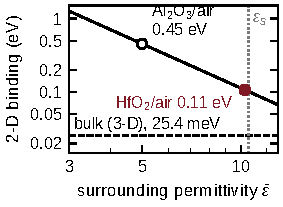
\includegraphics[width=\linewidth]{12_binding}\par
      \raggedright
      \src{Strict 2-D bound $4\,\mathrm{Ry}\,(m^*/m_0)/\bar\varepsilon^{\,2}$, $\bar\varepsilon = (\varepsilon_1 +
        \varepsilon_2)/2$ (\AlO{} $\approx 9$, \HfO{} 19.57, air 1). Grey: device stack; dotted: $\varepsilon_s$;
        dashed: bulk $E_D$. \lab{theory}; FACT-080.}
    \end{column}
  \end{columns}
  \takeaway{A W-independent route to fewer active donors in thin films; not computed here.}
\end{frame}

% ---------------------------------------------------------------------------------------------------------------------
\begin{frame}[t]{The largest uncertainties are not numerical}
  \twelveTop
  % plain tabular (not tabularx): tabularx typesets its body several times and would duplicate the footnote
  \begingroup\scriptsize
  \setlength{\tabcolsep}{4.2pt}
  \renewcommand{\arraystretch}{1.12}
  \begin{tabular}{@{}>{\raggedright\arraybackslash}p{2.75cm}>{\raggedright\arraybackslash}p{5.3cm}>{\raggedright\arraybackslash}p{1.25cm}>{\raggedright\arraybackslash}p{3.75cm}@{}}
    \toprule
    Source & Size or effect & Quantified & How it would be reduced \\
    \midrule
    One device per thickness & spread unknown; it enters every film-to-film difference (C026) & no &
      $\ge$10 devices per thickness, one run, dual sweeps \\
    Thickness values and definition & nominal values, method unknown; H--H or nominal: $\pm0.2$\,nm
      $\approx\pm40$\,mV in $\Vthcc$ at 2\,nm & partly & XRR and TEM on the same films; state the definition \\
    Crystalline PBE inputs for amorphous films & (001) slabs, OH termination; amorphous shift sealed (H-K); ML force
      check failed (C037) & partly & release of H-K; re-registered series, $\ge$2 seeds per endpoint \\
    Density-of-states convention at 2\,nm & quasi-2-D against 3-D $N_c$: 142\,mV in $\Vthcc$ (S1-05), a third to
      two thirds of a 6.3\,nm miss & yes & state it with every fitted charge \\
    PBE gap and functional & 0.89\,eV against 2.7--2.9\,eV measured\srefs{Walsh2008,Irmscher2014}: only differences
      used; HSE06/PBE ratio 1.06--1.11 (1\,nm): $+16$ to $+29$\,mV at 2\,nm
      & partly & optical gap against thickness; hybrid-functional W cell \\
    Extrapolated laws & computed to 1.96\,nm, used 3--7 times beyond; $\dEc(6.3\,\mathrm{nm}) = 0.050$--0.075\,eV over
      fit options & partly & optical gap, C--V flat band against thickness \\
    \bottomrule
  \end{tabular}\par\endgroup
  \src{Effects on $\Vthcc$ \lab{derived} (laws, audit A13); S1-05 \lab{computed} (ATLAS, seen before register revision
    2). Not limiting: registered DFT convergence, SCF force noise $\approx6\times10^{-5}$\,Ry/bohr per component, TCAD
    numerics $\approx0.7$\,\%. Non-identifiable threshold parameters (C018): Part 4.}
  \takeaway{Device statistics, thickness metrology and the $N_c$ convention dominate.}
\end{frame}

% 13_resources.tex -- Part 13, computational cost. Sources: research_monograph/appendices/MH_resources.tex
% (tab:mono-res-atlas, launch budgets, recorded totals, tab:mono-res-dft, memory, infrastructure, energy estimate);
% evidence/derived/atlas_usage.json (launches, wall time, non-zero exits, longest launch);
% research_record/05_DECISION_LOG.md (D-02 budget 52; D-03 budget 57 -> 71; D-13 200 more; D-58 C10 17/200, cap not
% raised); appendices/MG_corrections.tex T1 (C10 runs from 0061, 17 of 200 by 2026-10-14);
% chapters/13_dft_rev.tex sec:dft-resources (totals, laptop, 30-100 GB) and sec:dft-gpu line 1421 (GPU benchmark:
% the same 96-atom SCF, 9 min 16 s on one H100 NVL against 1 h 16 min on 16 CPU cores, factor 8.2; NOTE: the row
% pairing in tab:dft-timing, 1 h 48 min vs 9 min, mixes the 35 A and 15 A vacuum cells and is not used here);
% chapters/M04b_dft_numerics.tex sec:mono-dft-cost (N^3 scaling, 328 -> 680 bands, 3.6 GB, 82 GB for the
% single-process GPU relaxation); qe_workflow/cern_htcondor/results/resources.json (pool snapshot 2026-10-06) and the
% PWSCF WALL lines and GPU model lines of the scf/relax/bands outputs in qe_workflow/cern_htcondor/results/ (wall
% times and hardware re-checked 2026-10-15; every GPU row ran on an H100 NVL).
% Energy: ESTIMATE with assumed power figures (MH), not an audit. No sealed run (0075-0077) and no amorphous
% electronic quantity appears. Tables and one TikZ diagram only; no figure files.
% Note: frame bodies start with a command, never with a brace group (beamer would read a subtitle).
\providecommand{\thirteendense}{\setbeamerfont{itemize/enumerate body}{size=\footnotesize}%
  \setbeamerfont{itemize/enumerate subbody}{size=\footnotesize}}
\providecommand{\thirteenTop}{\vspace{-4mm}}
\providecommand{\thirteenAtlas}{\footnote[frame]{Silvaco, \citetitle{AtlasManual}}}
\providecommand{\thirteenNpw}{N_{\mathrm{pw}}}
\providecommand{\thirteenNb}{N_{\mathrm{b}}}
\providecommand{\thirteenNk}{N_{k}}
\providecommand{\thirteenHead}[1]{{\footnotesize\bfseries #1\par}\vspace{0.8mm}}
\providecommand{\thirteenX}{\,$\times$\,}
\providecommand{\thirteenx}{$\times$}

\partslide{Part 13}{Computational cost}

% ---------------------------------------------------------------------------------------------------------------------
\begin{frame}[t]{Device simulation is cheap; launch budgets limit it}
  \thirteenTop\thirteendense
  \begin{columns}[T,onlytextwidth]
    \begin{column}{0.58\textwidth}
      \thirteenHead{ATLAS launches in the public record\thirteenAtlas}
      {\footnotesize\setlength{\tabcolsep}{4.5pt}
      \begin{tabular}{@{}lrrr@{}}
        \toprule
        Study & Launches & \shortstack[r]{Wall\\time (h)} & \shortstack[r]{Exit\\$\neq 0$} \\
        \midrule
        Model V1 study      & 57 & 7.8 & 2 \\
        Model V2            &  3 & 0.5 & 0 \\
        Campaign C10        & 14 & 2.9 & 1 \\
        \midrule
        All public          & 74 & 11.1 & 3 \\
        \bottomrule
      \end{tabular}\par}
      \src{Silvaco ATLAS 5.28, 32-bit, local licence. Runs 0001--0057, 0058--0060, 0061--0074; wall times from
        \texttt{results/RUN\_INDEX.csv}; exit $\neq 0$: non-zero exit code; sealed runs 0075--0077 not included.
        Budgets: decision log D-02, D-03, D-13, D-58.}
    \end{column}
    \begin{column}{0.39\textwidth}
      \vspace{4.2mm}
      \begin{itemize}
        \item Launches run one at a time; the longest took 1.0\,h \lab{measured}. Each is a separately reviewed
          decision.
        \item Campaign C10 had used 17 launches by 14 October: the 14 in the table and the 3 sealed runs.
      \end{itemize}
    \end{column}
  \end{columns}
  \thirteenHead{ATLAS launch budget in the decision log (in order of date, not to scale)}
  \begin{tikzpicture}[x=1cm,y=1cm,font=\footnotesize]
    \foreach \a/\b in {0.25/3.15, 3.15/6.05, 6.05/10.0}
      \draw[rulegrey, line width=0.8pt, -{Stealth[length=1.6mm]}] (\a+0.15,0) -- (\b-0.17,0);
    \foreach \x/\d/\txt in {0.25/25 Sep/{budget: 52 launches},
        3.15/5 Oct/{budget 57 $\to$ 71},
        6.05/10 Oct/{200 more launches for C10}} {
      \fill (\x,0) circle (0.065);
      \node[anchor=south west, inner sep=0] at (\x-0.1,0.2) {\textbf{\d\ 2026}};
      \node[anchor=north west, inner sep=0] at (\x-0.1,-0.22) {\txt};
    }
    \fill[ntumaroon] (10.0,0) circle (0.085);
    \node[anchor=south west, inner sep=0] at (9.9,0.2) {\textbf{14 Oct 2026}};
    \node[anchor=north west, inner sep=0] at (9.9,-0.22)
      {\textcolor{ntumaroon}{17 of 200 used}; cap not raised};
  \end{tikzpicture}
  \takeaway{Device simulation costs hours; the scarce resource is the reviewed launch.}
\end{frame}

% ---------------------------------------------------------------------------------------------------------------------
\begin{frame}[t]{DFT to 4 October: about 8\,300 core-hours, 85--90 GPU-hours}
  \thirteenTop\thirteendense
  \begin{columns}[T,onlytextwidth]
    \begin{column}{0.545\textwidth}
      \thirteenHead{Quantum ESPRESSO\srefs{Giannozzi2009,Giannozzi2017} runs: measured wall times}
      {\scriptsize\setlength{\tabcolsep}{3pt}
      \begin{tabular}{@{}llr@{}}
        \toprule
        Step & Resources & Wall time \\
        \midrule
        80-atom W cell, relaxation                 & 32 CPU cores   & 23\,h 48\,min \\
        80-atom W cell, SCF, 4\thirteenx4\thirteenx4 $k$ & 32 CPU cores & 3\,h 03\,min \\
        1\,nm W film (96 atoms), SCF               & 16 CPU cores   &  2\,h 55\,min \\
        1\,nm film, bands                          & 16 CPU cores   &  4\,h 38\,min \\
        2\,nm W film (176 atoms), relax, 28 BFGS   & one H100 NVL   & 16\,h 49\,min \\
        2\,nm W film, final SCF                    & 33 CPU cores   &  8\,h 05\,min \\
        2\,nm film, bands                          & one H100 NVL   &  8\,h 22\,min \\
        0.695\,nm film, relaxation                 & one H100 NVL   &  9\,h 58\,min \\
        HSE06, 1\,nm film, SCF, 4 $k$ points       & one H100 NVL   &  4\,h 00\,min \\
        HSE06, bulk, SCF, 3\thirteenx3\thirteenx3 $q$ mesh & one H100 NVL & 4\,h 15\,min \\
        \bottomrule
      \end{tabular}\par}
      \src{Representative steps; PWSCF wall times in the output files. The 2\,nm W film and the 0.695\,nm film belong to the later
        jobs and are not in the totals.}
    \end{column}
    \begin{column}{0.425\textwidth}
      \thirteenHead{Recorded usage up to 4 October 2026}
      \begin{itemize}
        \item CERN: about 8\,300 weighted CPU core-hours and 85--90 GPU-hours; laptop: about 190 core-hours
          \lab{derived}.
        \item About 3\,000 of the core-hours and 50 GPU-hours were lost to failures, since fixed \lab{derived}.
        \item A laptop would need about six weeks for the useful work \lab{inferred} and could not run the 2\,nm
          and hybrid films (30--100\,GB).
        \item Energy estimate (not an audit) at 10\,W per core and 0.4\,kW per GPU \lab{assumed}:
      \end{itemize}
      \vspace{0.3mm}
      {\footnotesize\centering 8\,300\,h\thirteenX10\,W + 90\,h\thirteenX0.4\,kW $\approx$ 120\,kWh\par}
    \end{column}
  \end{columns}
  \takeaway{Estimated energy to 4 October: about 120\,kWh; later jobs are not yet totalled.}
\end{frame}

% ---------------------------------------------------------------------------------------------------------------------
\begin{frame}[t]{At 66--82\,GB, memory decided where the 176-atom film ran}
  \thirteenTop\thirteendense
  \begin{columns}[T,onlytextwidth]
    \begin{column}{0.53\textwidth}
      \thirteenHead{Plane-wave cost for a cell of $N$ atoms}
      {\centering$t_{\mathrm{it}} \propto \thirteenNb^{2}\,\thirteenNpw \propto N^{3}, \qquad
         M_{\psi} \propto \thirteenNb\,\thirteenNpw\,\thirteenNk \propto N^{2}\thirteenNk$\par}
      \vspace{0.8mm}
      {\scriptsize\color{inkgrey} $t_{\mathrm{it}}$: time per SCF iteration; $M_{\psi}$: wave-function memory;
        $\thirteenNb$, $\thirteenNpw$, $\thirteenNk$: bands, plane waves, $k$ points. Linear-scaling
        methods\sref{Goedecker1999} not used.\par}
      \vspace{1mm}
      \begin{itemize}
        \item 1\,nm $\to$ 2\,nm film: bands 328 $\to$ 680, plane waves +29\,\%; wave functions \thirteenx2.7,
          $\thirteenNb^{2}\thirteenNpw$ work \thirteenx5.5 \lab{derived}.
        \item 2\,nm film: 680\thirteenX327\,585\thirteenX16\,B = 3.6\,GB per $k$ point \lab{derived};
          \texttt{pw.x} estimates 82\,GB for the single-process GPU relaxation \lab{computed}; the final SCF needed
          66\,GB \lab{measured}. Hence a large-memory GPU or a distributed CPU run.
        \item HSE06, 1\,nm film: the default exact-exchange cutoff ran out of memory; 160\,Ry was used
          \lab{observed}.
      \end{itemize}
    \end{column}
    \begin{column}{0.44\textwidth}
      \thirteenHead{CERN GPU pool, 6 Oct 2026 \lab{observed}}
      {\footnotesize
      \begin{tabular}{@{}lr@{}}
        \toprule
        GPU model & GPUs \\
        \midrule
        H100 NVL & 144 \\
        H200 & 96 \\
        A100-PCIE-40GB & 72 \\
        Older (V100, V100S, T4) & 93 \\
        \midrule
        Total, on 79 nodes & 405 \\
        \bottomrule
      \end{tabular}\par}
      \src{HTCondor snapshot (\texttt{resources.json}); jobs from lxplus, data on EOS.}
      \vspace{1mm}
      \begin{itemize}
        \item A pure 1\,nm film SCF benchmark (96 atoms): 1\,h 16\,min on 16 CPU cores, 9\,min on one H100 NVL (\thirteenx8.2)
          \lab{measured}.
        \item About 0.8 GPU starts per hour \lab{observed}; two-GPU requests of the amorphous campaign matched no
          slot.
      \end{itemize}
    \end{column}
  \end{columns}
  \takeaway{For the large cells, memory and access to large GPUs, not core-hours, were the limits.}
\end{frame}

% 14_conclusions.tex -- Part 14, conclusions and next steps. Sources: research_monograph/chapters/M15_conclusions.tex
% (sec:concl-demonstrated, sec:concl-supported, sec:concl-inferred as re-sorted in Gate 6 (V9), tab:mono-concl-claims,
% sec:mono-concl-validation, outlook, keyresult); M01_introduction.tex (contributions paragraph, lines 94-104);
% M12_multiscale.tex (sec:mono-ms-explain, sec:mono-ms-reco, tab:mono-ms-budget); M14_audit.tex (findings and
% recommendations); M13_alternatives_uncertainty.tex (tab:mono-alt-floor: x7 / x1.02); M10_w_and_vacancies.tex
% (tab:mono-w-open); M11_amorphous_protocol.tex (prop:mono-hn, D-43); evidence/FACT_REGISTRY.tsv (FACT-004, 010d, 011d,
% 016, 017, 026c, 026d, 027, 030, 043, 050, 051, 101-103); evidence/CLAIM_SOURCE_MAP.tsv (C002, C003, C005, C007,
% C014, C018-C022, C024, C026, C029-C031, C037-C040, M001, M004, M007). No figure.
% No amorphous electronic quantity; no ATLAS result from stage S2 on. No e-mail address (none in the README).
% Note: frame bodies start with a command, never with a brace group (beamer would read a subtitle).
% Note: a p-cell that starts with \lab (a \color whatsit) needs \leavevmode, or it is set one line too low.
\partslide{Part 14}{Conclusions and next steps}

% local helpers of this section
\providecommand{\fourteenTop}{\vspace{-4mm}}
\providecommand{\fourteenC}[1]{{\tiny\color{inkgrey}#1}}
\providecommand{\fourteenData}{Data: Prof.\ M.-H.\ Lee's group, NTU; one device per thickness}
% group heading spanning a two-column table
\providecommand{\fourteenGroup}[1]{\multicolumn{2}{@{}l}{\footnotesize\textbf{#1}}\\[0.2mm]}

% ---------------------------------------------------------------------------------------------------------------------
\begin{frame}[t]{Seven results are demonstrated or computed within scope}
  \fourteenTop
  % plain tabular (not tabularx): tabularx typesets its body several times and would duplicate the footnotes
  \begingroup\scriptsize
  \setlength{\tabcolsep}{4pt}
  \renewcommand{\arraystretch}{1.08}
  \begin{tabular}{@{}>{\raggedright\arraybackslash}p{1.75cm}>{\raggedright\arraybackslash}p{11.9cm}@{}}
    \toprule
    \fourteenGroup{Demonstrated, or computed within a stated scope (crystalline cells, PBE, stated settings)}
    Devices
      & $\Vthcc = 0.662$, 0.644, 0.083\,V at 2.0, 6.3, 13.2\,nm, floors and on-currents: registered protocol, reproduced
        independently within rounding; non-uniform in thickness; 31.8\,nm does not switch off \lab{derived} \\
    Device models
      & Calibrations: each per-film model reproduces its own curve by construction; every out-of-sample threshold
        prediction for 6.3\,nm failed ($-0.29$, $-0.37$, $-0.23$\,V) \lab{falsified} \\
    Confinement
      & PBE gap opening $+2.25$, $+1.31$, $+0.90$, $+0.335$\,eV at $\tHH = 0.461$ (In$_8$(OH)$_{24}$), 0.695 (polar),
        0.930, 1.962\,nm; within 0.04 and 0.005\,eV of an independent calculation at 1 and
        2\,nm\sref[p.~21542]{Lin2022}; 84\,\% of the opening in the conduction band at 2\,nm; HSE06/PBE ratio
        1.06--1.11 at 1\,nm \lab{computed} \\
    Masses
      & Electron band-edge mass 0.154\,$\mzero$ in bulk, 0.203 and 0.279\,$\mzero$ at 1.96 and 0.93\,nm; no meaningful
        single hole mass \lab{computed}. Bulk Kane relation, no fit: 2\,nm mass within 1\,\%, 1\,nm mass 10\,\% too
        high \lab{derived} \\
    W, crystalline
      & On the 24d site; the W-5d-rich level is a resonance 1.2--1.8\,eV above the host band bottom, near $\EF$, at the
        computed filling; the earlier deep-donor reading was a band-count artefact (X1) \lab{computed} \\
    ML structures
      & The machine-learned amorphous structures failed their registered force check in the W first shell
        \lab{computed} \\
    H-N verdict
      & The registered H-N outcome cannot be a crossover verdict; this follows from the frozen rules (A37)
        \lab{derived} \\
    \bottomrule
  \end{tabular}\par\endgroup
  \src{A conclusion is listed under the weakest class of any of its parts; PBE results are not measurements of the
    device films. Ledger, by row: C002/C003/C026/C029; C014; C020/C021/C039; C039/C040/M004; C022; C037; M001.
    \fourteenData\sref{Januar2026}.}
  \takeaway{Firm results concern the devices and the rules; PBE results hold for crystalline cells.}
\end{frame}

% ---------------------------------------------------------------------------------------------------------------------
\begin{frame}[t]{Three results are strongly supported; five are conditional}
  \fourteenTop
  \begingroup\scriptsize
  \setlength{\tabcolsep}{4pt}
  \renewcommand{\arraystretch}{1.04}
  \begin{tabular}{@{}>{\raggedright\arraybackslash}p{1.75cm}>{\raggedright\arraybackslash}p{11.9cm}@{}}
    \toprule
    \fourteenGroup{Strongly supported}
    Contacts
      & A thickness-independent series resistance cannot create the trend: it would need 83\,\% of $\Vd$ at 2\,nm
        \lab{derived} \\
    Swing
      & The local swing of the three thinner films collapses against $\Id/I_{\mathrm{on}}$, in data and in simulation
        \lab{observed} \\
    Mobility
      & The saturation-formula peak reproduces the published mobilities with no free factor (5.09, 3.86, 27.40 against
        5.1, 3.73, 27.4\cmVs); the formula does not describe these curves as a mobility \lab{derived} \\
    \midrule
    \fourteenGroup{Inferred, derived under stated conditions, or computed but unresolved}
    Floor
      & Unlikely to be gate leakage: flat in $\Vg$, but no gate current recorded and the registered tests sealed
        \lab{inferred} \\
    Definition
      & The saturation formula is the leading candidate for the paper's mobility definition \lab{inferred}; the
        published values stay \textsc{unresolved} until the group confirms its recipe \\
    Threshold step
      & Of the measured 2.0--13.2\,nm step ($-0.579$\,V): 44\,\% by rigid transfer of the PBE $\dEc$ law ($-0.257$\,V),
        about 50\,\% in the earlier calibrated model, about 18\,\% as the audit's all-inputs-off counterfactual (A13).
        Not identifiable from transfer curves (C018): confinement alone does not account for the step \lab{inferred} \\
    6.3\,nm misses
      & The threshold stays flat from 2.0 to 6.3\,nm ($-0.018$\,V) where the computed shift implies about 0.2\,V, the
        direction and size of every miss; no cause is assigned \lab{derived} \\
    Vacancies
      & Crystalline, degenerately doped: a vacancy far from W costs 0.73\,eV more than in pure \InO{} (passes its
        threshold), next to W a further 0.53--0.56\,eV (significance unresolved); spin unassessed; not formation energies
        at device conditions; H-L is \textsc{unresolved} overall \lab{computed} \\
    \bottomrule
  \end{tabular}\par\endgroup
  \src{Ledger, by row: C019; C007; C030; C005; C031/C024; M007/C018; M007/C014; C038. Sealed, not shown: amorphous W
    and confinement (H-G, H-K, H-N per cell; D-43); shared-model transfer and floor tests (campaign completion).
    \fourteenData\sref{Januar2026}.}
\end{frame}

% ---------------------------------------------------------------------------------------------------------------------
\begin{frame}[t]{Seven contributions stand on the present evidence}
  \fourteenTop
  \begingroup\scriptsize
  \setlength{\tabcolsep}{4pt}
  \renewcommand{\arraystretch}{1.08}
  \begin{tabular}{@{}>{\raggedright\arraybackslash}p{0.25cm}>{\raggedright\arraybackslash}p{7.85cm}>{\raggedright\arraybackslash}p{1.6cm}>{\raggedright\arraybackslash}p{2.45cm}>{\centering\arraybackslash}p{0.65cm}@{}}
    \toprule
    & Contribution & Label & Condition & Part \\
    \midrule
    1 & A confinement series of crystalline \InO{} films (0.46--1.96\,nm): masses on a stated basis, band-edge
        partition, HSE06 check, laws with uncertainties
      & \leavevmode\lab{computed}\newline\lab{fitted} & crystalline (001), PBE, OH-terminated & 6, 7 \\
    2 & The mass increase is consistent with the bulk non-parabolicity, with no fit (1\,\% at 2\,nm, 10\,\% at
        1\,nm): one independent law, $\dEc(t)$, not two
      & \leavevmode\lab{derived} & crystalline & 7, 10 \\
    3 & W in crystalline \InO{} is a resonant donor at high filling; the earlier deep-donor reading is withdrawn
      & \leavevmode\lab{computed} & crystalline, PBE, one filling & 8 \\
    4 & A registered crystalline vacancy test (H-L), scored under frozen rules
      & \leavevmode\lab{computed} & unresolved overall & 9 \\
    5 & A fully specified blind protocol for amorphous films, and the finding that its central test, H-N, cannot
        return a crossover verdict
      & \leavevmode\lab{derived} & frozen rules; outcomes sealed & 11 \\
    6 & A quantitative account of how every failed 6.3\,nm prediction relates to the computed shift, all in the same
        direction, without assigning a cause
      & \leavevmode\lab{derived} & uses the device data & 10 \\
    7 & A reconciliation of the published\sref{Januar2026} and the derived device metrics
      & \leavevmode\lab{derived} & uses the device data & 2 \\
    \bottomrule
  \end{tabular}\par\endgroup
  \src{Labels and conditions as in the monograph's claim-status table. No claim is approved for publication: results
    that use the device curves need the fabrication group's agreement on permission, attribution, AI processing and
    authorship (meeting pending); the frozen registrations still need an external timestamp (DOI).}
  \takeaway{The strongest original result is computational and crystalline: the confinement series.}
\end{frame}

% ---------------------------------------------------------------------------------------------------------------------
\begin{frame}[t]{The decisive next steps are measurements}
  \fourteenTop
  \begingroup\scriptsize
  \setlength{\tabcolsep}{4pt}
  \renewcommand{\arraystretch}{1.12}
  \begin{tabular}{@{}>{\raggedright\arraybackslash}p{5.9cm}>{\raggedright\arraybackslash}p{7.75cm}@{}}
    \toprule
    \fourteenGroup{Measurements (by information per cost)}
    Floor against $\Vd$ from 0.1 to 0.7\,V on the existing chips, with the gate current recorded
      & ungated strip (floor $\times7$) or diffusion ($\times1.02$); gate leakage (C005) \\
    $\ge10$ devices per thickness from one run, dual sweeps
      & device spread against a film property; is 6.3\,nm on a smooth law? \\
    A dense series in about 1\,nm steps from 3 to 15\,nm, at 0, 2, 4\,\% W, capped and uncapped
      & a transition between 6.3 and 13.2\,nm against a smooth law; back-surface depletion \\
    Thickness metrology of the same films (XRR, TEM) and the stack order
      & the abscissa of every law: $\pm0.2$\,nm $\approx\pm40$\,mV in $\Vthcc$ at 2\,nm \\
    C--V flat band, optical gap, Hall density and photoemission band offsets against thickness
      & work function, affinity, fixed charge and $\dEc$, which act as one number in transfer curves (C018) \\
    \midrule
    \fourteenGroup{Calculations and registered work}
    W cells with a hybrid functional (HSE06) or PBE+$U$
      & does the W-5d level stay above the host edge? can W trap an electron? \\
    A density series of W cells (lower density)
      & does the filling pin $\EF$? is W ionised at device densities? \\
    Release of the sealed amorphous results under D-43
      & amorphous confinement (H-K) and W (H-G, H-N per cell) \\
    Completion of the registered device campaign (C10)
      & can one shared parameter set with computed inputs describe all films? \\
    \bottomrule
  \end{tabular}\par\endgroup
  \src{Also: a dipole-corrected SCF of the 0.695\,nm film; charged vacancy cells; for H-N, a re-registered series with
    $\ge2$ seeds per endpoint. Device model: carry one law, $\dEc(t)$, with its fit-option band, and state the
    $N_{\mathrm{c}}$ convention with every fitted charge. None of the measurements exists yet for these films.}
  \takeaway{First the floor against drain bias, device statistics and thickness metrology.}
\end{frame}

% ---------------------------------------------------------------------------------------------------------------------
{\setbeamertemplate{footline}{}
\begin{frame}[plain,noframenumbering]
  \begin{tikzpicture}[remember picture,overlay]
    \node[anchor=west,inner sep=0,text width=120mm,align=left] at ($(current page.west)+(10mm,6mm)$) {%
      {\LARGE\bfseries Thank you\par}
      \vspace{3mm}
      {\color{ntumaroon}\rule{30mm}{0.6pt}\par}
      \vspace{4mm}
      {\small\textbf{Mahmoud Elrasheedy}\par}
      \vspace{1mm}
      {\footnotesize National Taiwan University\par}
      \vspace{0.6mm}
      {\footnotesize Advisor: Prof.\ Chao-Hsin Wu \quad\textperiodcentered\quad Mentor: Mukul Kumar\par}
      \vspace{5mm}
      {\footnotesize Questions and comments are welcome.\par}
    };
    \node[anchor=south east,inner sep=0] at ($(current page.south east)+(-10mm,21mm)$) {\ntuemblem{16mm}};
    \draw[rulegrey,line width=0.4pt] ($(current page.south west)+(10mm,17mm)$) -- ($(current page.south east)+(-10mm,17mm)$);
    \node[anchor=north west,inner sep=0,text width=140mm,align=left] at ($(current page.south west)+(10mm,15mm)$) {%
      {\scriptsize\color{inkgrey} Device data: Prof.\ Min-Hung Lee's group, NTU (M.~Januar, Z.-F.~Luo; with
        K.-C.~Liu, Chang Gung University)\par}
    };
  \end{tikzpicture}
\end{frame}}

% 15_references.tex -- acknowledgements and full reference list (written by hand).
\begin{frame}{Acknowledgements}
  \begin{itemize}
    \item Prof.\ Chao-Hsin Wu (advisor) and Mukul Kumar (mentor), National Taiwan University.
    \item Prof.\ Min-Hung Lee's group, National Taiwan University (Dr.\ Mochamad Januar, Zhao-Feng Luo), for the
      device data and the published device study\sref{Januar2026}; Prof.\ Kou-Chen Liu, Chang Gung University.
    \item Computing: CERN HTCondor batch service (CPU and GPU nodes); Quantum ESPRESSO\srefs{Giannozzi2009,Giannozzi2017};
      Silvaco ATLAS\sref{AtlasManual}.
    \item Analysis workflow: all hypotheses and read-out rules were registered before the outcomes were known;
      computational execution and record keeping were assisted by AI coding agents, with every decision taken and
      logged by the author.
  \end{itemize}
\end{frame}

\begin{frame}[allowframebreaks]{References}
  \printbibliography[heading=none]
\end{frame}

% 16_backup.tex -- Backup slides (supplementary, for questions). Sources: research_monograph/chapters/
% M05_confinement_theory.tex (sec:mono-conf-kane, sec:mono-conf-subband, tab:mono-conf-test, sec:mono-conf-dos),
% M06_defect_theory.tex (sec:mono-defect-hydrogenic), M04_dft_theory.tex (sec:mono-dft-smearing, eq. mono-dft-mv),
% M04b_dft_numerics.tex (sec:mono-dft-align, eq. mono-dft-twostep), M09_masses_parameters.tex (tab:mono-mass-laws,
% tab:mono-mass-tcad, sec:mono-mass-tcad), M02_questions.tex (tab:mono-q-map), M08_c10_campaign.tex (tab:mono-c10-hyp,
% tab:mono-c10-s1, sec:mono-c10-s1), M10_w_and_vacancies.tex (H-L), M11_amorphous_protocol.tex (tab:mono-am-tests,
% prop:mono-hn), M12_multiscale.tex (fig:mono-ms-chain, labels); appendices/MG_corrections.tex (X1-X13, R1, V1-V12;
% V12: MV weights as implemented in QE, 0.40 at mu, never negative, maximum 1.083 at x = -sqrt2, printed 8b occupations
% up to 1.074); evidence/FACT_REGISTRY.tsv (FACT-004, 005, 014, 015, 025, 027, 030, 045, 071, 080);
% evidence/CLAIM_SOURCE_MAP.tsv (C034 amorphous force-only screen, C039); evidence/derived/defect_estimates.json;
% evidence/derived/confinement_analysis.json; qe_workflow/analysis_2026-10-13_full/bands_masses/out/b04_tcad.json.
% Literature anchors: Fan2021 for 3.05 eV and 4.3 eV (M09:170; report 02c:191, 04:166/206), Stokey2021 p. 225102-1 for
% 0.208 m0 (M09:82).
% Blind rules: no sealed outcome, no amorphous electronic quantity, no ATLAS result from S2 on (S1-05 was seen before the
% register freeze). Figures: none (equations, tables and one TikZ schematic).
% Note: every frame body starts with a command, never with a brace group (beamer would read a frame subtitle).
\providecommand{\sixteendense}{\setbeamerfont{itemize/enumerate body}{size=\footnotesize}%
  \setbeamerfont{itemize/enumerate subbody}{size=\footnotesize}}
\providecommand{\sixteenEq}{\setlength{\abovedisplayskip}{2pt}\setlength{\belowdisplayskip}{2pt}%
  \setlength{\abovedisplayshortskip}{1pt}\setlength{\belowdisplayshortskip}{1pt}\setlength{\jot}{2pt}}
\providecommand{\sixteenVV}{\bar{\bar{V}}}
\providecommand{\sixteenAum}{\si{A/\micro\metre}}
\providecommand{\sixteenNc}{N_{\mathrm{c}}}
\providecommand{\sixteenNv}{N_{\mathrm{v}}}
\providecommand{\sixteenTop}{\vspace{-4mm}}
% evidence label at the size of the surrounding text (for \src lines, where \lab would print larger than the text)
\providecommand{\sixteenSrcLab}[1]{{\color{inkgrey}[\textsc{\MakeLowercase{#1}}]}}

\partslide{Backup}{Supplementary slides}

% ---------------------------------------------------------------------------------------------------------------------
\begin{frame}{A confined Kane band is heavier in-plane by the factor $1+2\alpha E_1$}
  \sixteenTop\sixteendense\sixteenEq
  \begin{columns}[T,onlytextwidth]
    \begin{column}{0.51\textwidth}
      \footnotesize
      \textbf{Bulk}\sref{Kane1957}: $E(1+\alpha E) = \hbar^2k^2/2m_b$, $E$ above the minimum.\par
      \vspace{0.8mm}
      \textbf{Film} of width $t$: quantise $k_z = n\pi/t$, keep $k_\parallel$:
      \[ E(1+\alpha E) = \varepsilon_n + \frac{\hbar^2k_\parallel^2}{2m_b},\quad
         \varepsilon_n = \frac{\hbar^2\pi^2n^2}{2m_bt^2} = \frac{0.376\,\mathrm{eV\,nm^2}}{(m_b/m_0)\,t^2}\,n^2 \]
      \textbf{Subband edge} ($k_\parallel = 0$) and local thickness exponent:
      \[ E_n = \frac{\sqrt{1+4\alpha\varepsilon_n}-1}{2\alpha},\qquad
         p(E) \equiv -\frac{d\ln E}{d\ln t} = 2\,\frac{1+\alpha E}{1+2\alpha E} \]
      \textbf{In-plane}, $k_\parallel \to 0$: $(1+2\alpha E_1)\,dE = (\hbar^2/m_b)\,k_\parallel dk_\parallel$, hence
      \[ m_\parallel = m_b\,(1+2\alpha E_1),\qquad \alpha_\parallel = \alpha/(1+2\alpha E_1) \]
    \end{column}
    \begin{column}{0.46\textwidth}
      \begingroup\scriptsize
      \setlength{\tabcolsep}{3.5pt}
      \renewcommand{\arraystretch}{1.1}
      \begin{tabular}{@{}l c c c c@{}}
        \toprule
        $\tHH$ & $E_1 = \dEc$ & $m_\parallel$ ($m_0$) & $\alpha_\parallel$ (eV$^{-1}$) & $p(E_1)$ \\
        (nm) & (eV) & DFT\,/\,Kane & DFT\,/\,Kane & \\
        \midrule
        1.962 & 0.281 & 0.203\,/\,0.204 & 0.47\,/\,0.44 & 1.75 \\
        0.930 & 0.848 & 0.279\,/\,0.306 & 0.36\,/\,0.29 & 1.50 \\
        \bottomrule
      \end{tabular}\par\endgroup
      \src{DFT columns \sixteenSrcLab{computed}; Kane columns from bulk $m_b$, $\alpha$ and the computed $\dEc$,
        nothing adjusted \sixteenSrcLab{derived}. FACT-027.}
      \vspace{0.4mm}
      \begin{itemize}
        \item Inputs: $m_b = 0.1541\,m_0$, $\alpha = 0.58$\,eV$^{-1}$ (0.55--0.63), fitted up to 0.45\,eV
          \lab{computed}.
        \item The two-band $\alpha$ with the PBE gap would be 0.81\,eV$^{-1}$; $\alpha$ is taken from the fit.
        \item $E_P$ depends on the functional: masses are computed, not scaled from gaps \lab{derived}.
        \item $(E_2 - E_1)/E_1$ = 2.56 at 2\,nm and 1.77 at 1\,nm, below the parabolic 3 \lab{computed}.
      \end{itemize}
    \end{column}
  \end{columns}
  \takeaway{The mass law and the $\dEc$ law are one input to about 10\,\%, not two.}
\end{frame}

% ---------------------------------------------------------------------------------------------------------------------
\begin{frame}{Hydrogenic donor: 25\,meV in bulk, four times that in strict 2-D}
  \sixteenTop\sixteendense\sixteenEq
  \begin{columns}[T,onlytextwidth]
    \begin{column}{0.52\textwidth}
      \footnotesize
      \textbf{Bulk}, potential $-e^2/(4\pi\varepsilon_0\varepsilon_s r)$, and Mott criterion:
      \[ E_D = \frac{m^*/m_0}{\varepsilon_s^2}\,\mathrm{Ry},\qquad a_B^* = \frac{\varepsilon_s}{m^*/m_0}\,a_0,\qquad
         n_c^{1/3}a_B^* \approx 0.26 \]
      \textbf{Strict 2-D}; the surroundings screen beyond $r_0$\srefs{Bastard1981b,Cudazzo2011}:
      \[ E_D^{\mathrm{2D}} = 4E_D,\quad a_{\mathrm{2D}} = a_B^*/2;\qquad
         E_D^{\mathrm{2D}} \le 4\,\mathrm{Ry}\,(m^*/m_0)/\bar\varepsilon^{\,2} \]
      {\scriptsize $r_0 = \varepsilon_s t/(\varepsilon_1+\varepsilon_2)$; $\varepsilon_{1,2}$ below, above the film;
        $\bar\varepsilon$ their mean.\par}
      \vspace{0.6mm}
      \begingroup\scriptsize
      \setlength{\tabcolsep}{3.2pt}
      \begin{tabular}{@{}l c c c c c c@{}}
        \toprule
        $m^*$ basis & $m^*/m_0$ & $E_D$ & $a_B^*$ & $n_c$ & $E_D^{\mathrm{2D}}$ & $a_{\mathrm{2D}}$ \\
         & & (meV) & (nm) & (cm$^{-3}$) & (meV) & (nm) \\
        \midrule
        measured\sref[p.~225102-1]{Stokey2021} & 0.208 & 25.4 & 2.68 & $9.1\times10^{17}$ & 101.7 & 1.34 \\
        PBE band edge & 0.154 & 18.8 & 3.62 & $3.7\times10^{17}$ & 75.3 & 1.81 \\
        \bottomrule
      \end{tabular}\par\endgroup
      \src{Ry = 13.606\,eV, $a_0 = 0.0529$\,nm, $\varepsilon_s = 10.55$; PBE mass: this work. FACT-080
        \sixteenSrcLab{derived}.}
    \end{column}
    \begin{column}{0.44\textwidth}
      \begin{itemize}
        \item Crystalline W cells, 1.4--3.0$\times10^{21}$\cmcu{} ($1500$--$3300\,n_c$): no bound state
          \lab{derived}.
        \item At $t = 2$\,nm ($0.75\,a_B^*$) confinement roughly doubles $E_D$; \AlO{}/air ($\bar\varepsilon = 5$):
          up to 0.45\,eV; \HfO{}/air ($\bar\varepsilon = 10.3$): 0.11\,eV \lab{theory}.
        \item The 2\,nm \AlO{} is as thick as $r_0 \approx 2.1$\,nm and $a_{\mathrm{2D}} \approx 1.3$\,nm: between
          the cases, nearer \HfO{}/air far out (review correction V6) \lab{theory}.
        \item Above the LO-phonon energy, static $\varepsilon_s$ and parabolic $m^*$ understate the binding;
          deactivation was predicted and observed in Si nanowires\srefs{Diarra2007,Bjork2009}.
      \end{itemize}
    \end{column}
  \end{columns}
  \takeaway{Thin films may activate fewer donors without W-specific chemistry; not computed here.}
\end{frame}

% ---------------------------------------------------------------------------------------------------------------------
\begin{frame}{Cold smearing trades an $O(\sigma^3)$ error for weights above one}
  \sixteenTop\sixteendense\sixteenEq
  \begin{columns}[T,onlytextwidth]
    \begin{column}{0.47\textwidth}
      \footnotesize
      Weights $f = \tilde f(x)$, $x = (\varepsilon-\mu)/\sigma$; $F = E - \sigma S$ is variational, so forces
      are derivatives of $F$\sref{Mermin1965}. Marzari--Vanderbilt (MV)\sref{Marzari1999}, as in Quantum ESPRESSO:
      \begin{align*}
        \tilde\delta(x) &= \pi^{-1/2}\,e^{-(x+a)^2}\,\big(2+\sqrt2\,x\big),\quad a = 1/\sqrt2,\\
        \tilde f(x) &= \int_x^\infty\!\tilde\delta\,dx' = \tfrac12\,\mathrm{erfc}(y) + \frac{e^{-y^2}}{\sqrt{2\pi}},
          \quad y = x+a .
      \end{align*}
      \vspace{0.6mm}
      \begingroup\scriptsize
      \setlength{\tabcolsep}{2.5pt}
      \renewcommand{\arraystretch}{1.08}
      \begin{tabular}{@{}l l l l@{}}
        \toprule
        Family & $\tilde f(x)$ & in $[0,1]$ & energy error \\
        \midrule
        Fermi--Dirac & $1/(e^x+1)$ & yes & physical, $\sigma = \kT$ \\
        Gaussian & $\tfrac12\mathrm{erfc}(x)$ & yes & $O(\sigma^2)$ \\
        Methfessel--Paxton\sref{Methfessel1989} & Hermite & no & no $\sigma^2$ term \\
        MV & above & no & $O(\sigma^3)$ \\
        \bottomrule
      \end{tabular}\par\endgroup
    \end{column}
    \begin{column}{0.51\textwidth}
      \begin{itemize}
        \item MV weight 0.40 at $x = 0$, never negative; above one below $\mu$, at most 1.083 at $x = -\sqrt2$
          \lab{derived}; printed 8b W-cell occupations reach 1.074 \lab{computed}.
        \item MV 0.01\,Ry = 136\,meV (crystalline W cells, amorphous W relaxations); Gaussian 0.005--0.001\,Ry;
          $\kT = 25.85$\,meV.
        \item W-5d counts (0.09--0.43\,e): projections of MV-weighted states, not a W charge \lab{computed}.
        \item MV to Gaussian 0.005\,Ry, one relaxed amorphous 1.0\,nm W cell (force-only): every force component
          changes by at most $2.4\times10^{-4}$\,Ry/bohr \lab{computed}.
      \end{itemize}
      \src{Review correction V12; record correction X11; force-only screen: ledger C034.}
    \end{column}
  \end{columns}
  \takeaway{MV weights are integration weights; occupations need narrow Gaussian smearing.}
\end{frame}

% ---------------------------------------------------------------------------------------------------------------------
\begin{frame}{Two-step alignment carries the bulk edge into the slab}
  \sixteendense\sixteenEq\toggletrue{blx@useprefix}% print "Van de Walle" in the footnote (local to this frame)
  \begin{columns}[T,onlytextwidth]
    \begin{column}{0.44\textwidth}
      \centering
      \begin{tikzpicture}[x=0.93mm,y=0.7mm,font=\scriptsize,>={Stealth[length=1.5mm]}]
        % bulk cell
        \draw[line width=0.5pt,dashed] (0,8) -- (14,8);
        \draw[line width=0.7pt] (0,26) -- (14,26);
        \node[anchor=south west,inner sep=1pt] at (0,26) {$\Ec^{\mathrm{bulk}}$};
        \node[anchor=north west,inner sep=1pt] at (0,7) {$\sixteenVV^{\,\mathrm{bulk}}$};
        \draw[<->,line width=0.5pt] (10,8.6) -- (10,25.4) node[midway,right=0.2mm] {(b)};
        % slab: planar average (grey) and macroscopic average (dashed)
        % the oscillation starts at x = 25 (on its average) so that the grey (b) arrow at x = 23.5 stays clear of it
        \draw[inkgrey,line width=0.4pt,domain=25:42,samples=103,smooth] plot (\x,{8-5*cos(360*(\x-22)/4)});
        \draw[inkgrey,line width=0.4pt] (42,3) .. controls (45.5,3) and (46,50) .. (50,50);
        \draw[line width=0.5pt,dashed] (22,8) -- (42,8);
        \draw[line width=0.7pt] (50,50) -- (66,50);
        \node[anchor=south,inner sep=1pt] at (60,50) {$E_{\mathrm{vac}}$};
        % bulk-like edge placed on the slab interior average
        \draw[inkgrey,line width=0.5pt,dashed] (22,26) -- (42,26);
        \draw[<->,inkgrey,line width=0.5pt] (23.5,8.6) -- (23.5,25.4) node[midway,right=0.2mm] {(b)};
        \node[anchor=north,inner sep=1pt,text=inkgrey] at (33,25.4) {bulk-like $\Ec$};
        % slab CBM
        \draw[ntumaroon,line width=0.8pt] (22,35) -- (42,35);
        \node[anchor=south,inner sep=1pt,text=ntumaroon] at (31,35) {$E_{\mathrm{CBM}}^{\mathrm{slab}}$};
        \draw[<->,ntumaroon,line width=0.6pt] (39,26.6) -- (39,34.4);
        \node[anchor=west,inner sep=1pt,text=ntumaroon] at (39.5,30.5) {$\dEc$};
        % terms (a) and (c) on the vacuum scale
        \draw[dotted,line width=0.5pt] (42,8) -- (58,8);
        \draw[dotted,line width=0.5pt] (42,35) -- (64,35);
        \draw[<->,line width=0.5pt] (58,8.6) -- (58,49.4) node[pos=0.3,left=0.2mm] {(c)};
        \draw[<->,line width=0.5pt] (64,35.6) -- (64,49.4) node[midway,left=0.2mm] {(a)};
        \node[anchor=north west,inner sep=1pt] at (46.5,7.5) {$\sixteenVV^{\,\mathrm{slab}}_{\mathrm{int}}$};
        \node[text=inkgrey] at (7,-7) {bulk};
        \node[text=inkgrey] at (32,-7) {slab interior};
        \node[text=inkgrey] at (60,-7) {vacuum};
      \end{tikzpicture}\par
      \raggedright
      \src{Schematic. Grey: planar average $\bar V(z)$; dashed: its average $\sixteenVV$ over one period $l = a/2$
        along [001]. The 1\,nm $\dEv$ value: record correction X2.}
    \end{column}
    \begin{column}{0.52\textwidth}
      \footnotesize
      \[ \dEc(t) = \underbrace{\big[E_{\mathrm{CBM}}^{\mathrm{slab}} - E_{\mathrm{vac}}\big]}_{\text{(a)}}
         - \underbrace{\big[\Ec^{\mathrm{bulk}} - \sixteenVV^{\,\mathrm{bulk}}\big]}_{\text{(b)}}
         - \underbrace{\big[\sixteenVV^{\,\mathrm{slab}}_{\mathrm{int}} - E_{\mathrm{vac}}\big]}_{\text{(c)}} \]
      {\scriptsize Two-step method\srefs{VandeWalle1987,Baldereschi1988}; likewise $\dEv$ (signed, negative =
        downwards), and $\dEg = \dEc - \dEv$.\par}
      \vspace{-0.3mm}
      \begin{itemize}
        \item 2\,nm film, interior flat within 8\,meV: $\dEc = +0.281$, $\dEv = -0.054$\,eV (share 0.84);
          second route $-0.049$\,eV \lab{computed}.
        \item 1\,nm film, no bulk-like interior, same termination: $\dEc(1) = \dEc(2) + \mathrm{EA}(2) - \mathrm{EA}(1)$,
          $\dEv(1) = \dEv(2) + \mathrm{IP}(2) - \mathrm{IP}(1)$; $+0.848$ and $-0.052$\,eV (share 0.94) \lab{computed}.
        \item Check: $0.8477 + 0.0521 = 0.8998$\,eV $= \dEg(1\,\mathrm{nm})$.
      \end{itemize}
    \end{column}
  \end{columns}
  \takeaway{Alignment needs a bulk-like interior; the 1\,nm edges rest on the 2\,nm alignment.}
\end{frame}

% ---------------------------------------------------------------------------------------------------------------------
\begin{frame}{Device decks add PBE increments to literature bulk anchors}
  \sixteenTop\sixteendense
  \begingroup\scriptsize
  \setlength{\tabcolsep}{4pt}
  \renewcommand{\arraystretch}{0.94}
  \begin{tabular*}{\textwidth}{@{\extracolsep{\fill}}l l c c c l@{}}
    \toprule
    Quantity & Rule ($t$ = H--H thickness in nm; fitted at 0.695--1.962\,nm) & 2.0\,nm & 6.3\,nm & 13.2\,nm & Label \\
    \midrule
    $\dEg$ (eV) & $0.8147\,t^{-1.3155}$ & 0.327 & 0.072 & 0.027 & \lab{fitted} \\
    $\dEc$ (eV) & $0.7018\,t^{-1.3176}$ (frozen campaign law) & 0.282 & 0.062 & 0.023 & \lab{fitted} \\
    $\Delta m$ ($m_0$) & $0.1114\,t^{-1.2611}$ (deck basis) & 0.046 & 0.011 & 0.004 & \lab{fitted} \\[0.6mm]
    $\Eg$ (eV) & $3.05 + \dEg$ & 3.377 & 3.122 & 3.077 & \lab{derived} \\
    Affinity $\chi$ (eV) & $4.3 - \dEc$ & 4.019 & 4.238 & 4.277 & \lab{derived} \\
    $m^*$ ($m_0$) & $0.208 + \Delta m$ & 0.255 & 0.219 & 0.212 & \lab{derived} \\
    $\sixteenNc$ (cm$^{-3}$) & quasi-2-D $N_{\mathrm{2D}}/t$ at 2.0\,nm; 3-D otherwise & $1.373\times10^{19}$
      & $2.57\times10^{18}$ & $2.46\times10^{18}$ & \lab{derived} \\
    $\sixteenNv$ (cm$^{-3}$) & fixed; holes are not solved & $10^{19}$ & $10^{19}$ & $10^{19}$ & \lab{assumed} \\
    \bottomrule
  \end{tabular*}\par\endgroup
  {\scriptsize Derived = anchor + fitted increment; anchors: another sputtered IWO device\sref{Fan2021}, measured
    \InO{} mass\sref[p.~225102-1]{Stokey2021}.\par}
  \src{3.05\,eV: optical gap; 4.3\,eV: composition-mixing estimate. M09; b04\_tcad.json; $\dEc$ law fit3; campaign C10.}
  \begin{itemize}
    \item 6.3 and 13.2\,nm extrapolate the laws: $\dEc(6.3\,\mathrm{nm})$ = 0.050--0.075\,eV over the fit options
      \lab{fitted}; the campaign decks match to 0.11\,meV ($\Eg$, $\chi$), $0.0002\,m_0$, 0.1\,\% ($\sixteenNc$)
      \lab{computed}.
    \item Not in the decks: Kane factor of $\sixteenNc$ ($+5.7$\,\%), HSE ratio ($+6$ to $+11$\,\% in $\dEg$), computed
      $\sixteenNv \approx 2\times10^{21}$\cmcu.
  \end{itemize}
  \takeaway{Only differences come from PBE; absolute gap, affinity and mass are literature anchors.}
\end{frame}

% (The register table, H-A to H-N with criteria and status, is in sections/16b_backup_register.tex.)

% ---------------------------------------------------------------------------------------------------------------------
\begin{frame}{Record corrections X1--X13, review corrections V1--V12 apply}
  \begin{columns}[T,onlytextwidth]
    \begin{column}{0.495\textwidth}
      \begingroup\scriptsize
      \textbf{Record corrections} (logs, ledger, baseline report)\par
      \vspace{0.6mm}
      \setlength{\tabcolsep}{3pt}
      \renewcommand{\arraystretch}{1.07}
      \begin{tabularx}{\linewidth}{@{}l>{\raggedright\arraybackslash}X@{}}
        \toprule
        X1 & W level resonant, 1.2--1.8\,eV above $\Ec$ (band count) \\
        X2 & 1\,nm $\dEv = -0.052$, not $-0.056$\,eV (IP-difference sign) \\
        X3 & 2\,nm IWO final SCF: job 12835211, not 12835131 \\
        X4 & 0.51\,nm film relaxes to In$_8$(OH)$_{24}$; 0.695\,nm polar \\
        X5 & device model V1: a calibration, not a validation \\
        X6 & every mass names its fit basis \\
        X7 & bulk W moments 0.62 (24d), 0.74\,$\mu_{\mathrm{B}}$ (8b): not claimed \\
        X8 & MACE structures: starting points, not validated \\
        X9 & bulk W cell donates $2.7\times10^{21}$, not $5.5\times10^{21}$\cmcu \\
        X10 & 0.695\,nm polar; VB top on OH at 0.461, 0.695\,nm \\
        X11 & L\"owdin W-5d counts are not the W charge \\
        X12 & laws on relaxed H--H thickness, not Lin labels \\
        X13 & 0.8\,nm W restart not reproducible \\
        \bottomrule
      \end{tabularx}\par\endgroup
    \end{column}
    \begin{column}{0.475\textwidth}
      \begingroup\scriptsize
      \textbf{Review corrections} (Gate-6 review of the monograph)\par
      \vspace{0.6mm}
      \setlength{\tabcolsep}{3pt}
      \renewcommand{\arraystretch}{1.07}
      \begin{tabularx}{\linewidth}{@{}l>{\raggedright\arraybackslash}X@{}}
        \toprule
        V1 & SCF force noise $6\times10^{-5}$\,Ry/bohr per component \\
        V2 & cell relaxations by BFGS, not Wentzcovitch \\
        V3 & 38\,meV excess of the 2\,nm $\dEv$: unexplained \\
        V4 & envelope model: not predictive, not refuted \\
        V5 & Kane mass relation: 1\,\% at 2\,nm, 10\,\% at 1\,nm \\
        V6 & 0.45\,eV donor binding only for \AlO/air \\
        V7 & $E_F$ at the resonance: not evidence of pinning \\
        V8 & 2\,\% W active: $6\times10^{20}$--$1.8\times10^{21}$\cmcu; scale only \\
        V9 & conclusions re-sorted to their weakest class \\
        V10 & one subband at 2\,nm; one or two at 6.3\,nm \\
        V11 & smaller items (HSE ratio model 0.98--1.16, \ldots) \\
        V12 & MV weights: 0.40 at $\mu$, never negative, at most 1.083 \\
        \bottomrule
      \end{tabularx}\par\endgroup
    \end{column}
  \end{columns}
  \src{Appendix MG of the monograph lists each superseded statement next to its correction, with device-model and data
    entries, wording errata and disclosures; X lines also stay in the dated logs. R1: a proposed sign correction was
    re-checked and rejected (convention mix). X13: ledger C036.}
  \takeaway{A correction is accepted only if it names the error and its evidence.}
\end{frame}

% ---------------------------------------------------------------------------------------------------------------------
\begin{frame}{The quasi-2-D $N_{\mathrm{c}}$ convention outweighs the Kane factor}
  \sixteenTop\sixteendense\sixteenEq
  \begin{columns}[T,onlytextwidth]
    \begin{column}{0.48\textwidth}
      \footnotesize
      \textbf{Three dimensions}, parabolic, 300\,K:
      \[ \sixteenNc = 2\Big(\frac{2\pi m_b\kT}{h^2}\Big)^{3/2} = 2.509\times10^{19}\,(m_b/m_0)^{3/2}\ \mathrm{cm^{-3}} \]
      \textbf{Kane band}, to first order in $\alpha E$, with the Boltzmann average $\langle E\rangle = \tfrac32\kT$:
      \begin{align*}
        g(E) &\propto [E(1+\alpha E)]^{1/2}(1+2\alpha E) \approx E^{1/2}\big(1+\tfrac52\alpha E\big),\\
        \sixteenNc^{\mathrm{Kane}} &\approx \sixteenNc\big(1+\tfrac{15}{4}\,\alpha\kT\big) = 1.056\,\sixteenNc
          \quad(\alpha = 0.58\,\mathrm{eV^{-1}})
      \end{align*}
      \textbf{Quasi two dimensions}, one subband:
      \[ N_{\mathrm{2D}} = \frac{m_\parallel\kT}{\pi\hbar^2},\qquad \sixteenNc^{\mathrm{q2D}} = N_{\mathrm{2D}}/t \]
      {\scriptsize $N_{\mathrm{2D}} = 1.66\times10^{12}$\cmsq{} ($0.154\,m_0$), $2.19\times10^{12}$\cmsq{} ($0.203\,m_0$, 2\,nm);
        in-plane non-parabolicity adds $2\alpha_\parallel\kT$ = 2.4\,\% at 2\,nm \lab{derived}.\par}
    \end{column}
    \begin{column}{0.49\textwidth}
      \begin{itemize}
        \item Kane factor 1.056; full integral $+5.7$\,\% \lab{derived}; not in the decks.
        \item Register convention (amendment A13), 2.0\,nm, deck mass: $1.373\times10^{19}$ against
          $3.218\times10^{18}$\cmcu{} (3-D), factor 4.27: $\kT\ln 4.27 = 38$\,meV for free carriers \lab{derived}.
        \item One subband ($E_2-E_1 = 0.72$\,eV at 1.962\,nm) \lab{computed}: a DOS substitution, not 2-D statistics.
        \item Stage S1 check S1-05, seen before the freeze: 3-D at 2.0\,nm moved $\Vthcc$ by $+142$\,mV against
          $+40$ to $+70$\,mV registered: \textbf{failed} \lab{computed}.
        \item Audit (amendment A13): $+37.5$\,mV statistics, $+89.5$\,mV tail charge, the rest band bending, free
          carriers, lateral channel; slope factor about 3.5, not 1.47 \lab{computed}.
      \end{itemize}
    \end{column}
  \end{columns}
  \takeaway{Every fitted trap density or fixed charge must name its $N_{\mathrm{c}}$ convention.}
\end{frame}

\end{document}
